\documentclass[a4paper,12pt]{article}[abntex2]
\bibliographystyle{abntex2-alf}


% Definições de layout e formatação
\usepackage[a4paper, left=3.0cm, top=3.0cm, bottom=2.0cm, right=2.0cm]{geometry} % Personalização das margens do documento
\usepackage{setspace} % Controle do espaçamento entre linhas
\onehalfspacing % Espaçamento entre linhas de 1,5
\usepackage{indentfirst} % Indentação do primeiro parágrafo das seções
\usepackage{newtxtext} % Substitui a fonte padrão pela Times Roman
\usepackage{titlesec} % Personalização dos títulos de seções
\usepackage{ragged2e} % Melhor controle de justificação do texto
\usepackage[portuguese]{babel} % Adaptação para o português (nomes e hifenização)
\usepackage{multirow}

% Pacotes de cabeçalho, rodapé e títulos
\usepackage{fancyhdr} % Customização de cabeçalhos e rodapés
\setlength{\headheight}{14.49998pt} % Altura do cabeçalho
\pagestyle{fancy}
\fancyhf{} % Limpa cabeçalho e rodapé
\rhead{\thepage} % Página no canto direito do cabeçalho

% Pacotes para tabelas
\usepackage{booktabs} % Melhora a qualidade das tabelas
\usepackage{tabularx} % Permite tabelas com larguras de colunas ajustáveis
\usepackage{float} % Melhor controle sobre o posicionamento de figuras e tabelas

% Pacotes para gráficos e imagens
\usepackage{graphicx} % Suporte para inclusão de imagens

\usepackage[utf8]{inputenc}
\usepackage{listingsutf8}

\lstset{
    language=R,                      
    basicstyle=\ttfamily\scalefont{1.0},
    keywordstyle=\color{blue},       
    stringstyle=\color{red},         
    commentstyle=\color{green},      
    numbers=left,                    
    numberstyle=\tiny\color{gray},   
    stepnumber=1,                    
    numbersep=5pt,                   
    backgroundcolor=\color{lightgray!10}, 
    frame=single,                    
    breaklines=true,                 
    captionpos=b,                    
    keepspaces=true,                 
    showspaces=false,                
    showstringspaces=false,          
    showtabs=false,                  
    tabsize=2,
     literate={á}{{\'a}}1
             {é}{{\'e}}1
             {í}{{\'i}}1
             {ó}{{\'o}}1
             {ú}{{\'u}}1
             {Ú}{{\'U}}1
             {â}{{\^a}}1
             {ê}{{\^e}}1
             {î}{{\^i}}1
             {ô}{{\^o}}1
             {û}{{\^u}}1
             {ã}{{\~a}}1
             {õ}{{\~o}}1
             {ç}{{\c{c}}}1,
}


% Pacotes para unidades e formatação numérica
\usepackage{siunitx} % Tipografia de unidades do Sistema Internacional e formatação de números
\sisetup{
  output-decimal-marker = {,},
  inter-unit-product = \ensuremath{{}\cdot{}},
  per-mode = symbol
}
\DeclareSIUnit{\real}{R\$}
\newcommand{\real}[1]{R\$#1}

% Pacotes para hiperlinks e referências
\usepackage{hyperref} % Suporte a hiperlinks
\usepackage{footnotehyper} % Notas de rodapé clicáveis em combinação com hyperref
\hypersetup{
    colorlinks=true,
    linkcolor=black,
    filecolor=magenta,      
    urlcolor=cyan,
    citecolor=black,        
    pdfborder={0 0 0},
}
\makeatletter
\def\@pdfborder{0 0 0} % Remove a borda dos links
\def\@pdfborderstyle{/S/U/W 1} % Estilo da borda dos links
\makeatother

% Pacotes para texto e outros
\usepackage{lipsum} % Geração de texto dummy 'Lorem Ipsum'
\usepackage[normalem]{ulem} % Permite o uso de diferentes tipos de sublinhados sem alterar o \emph{}

\begin{document}

\begin{titlepage}
    \centering
    \vspace*{1cm}
    \Large\textbf{INSPER – INSTITUTO DE ENSINO E PESQUISA}\\
    \Large ECONOMIA\\
    \vspace{1.5cm}
    \Large\textbf{Caderno}\\
    \textbf{Direito e Economia das Políticas Públicas}\\
    \vspace{1.5cm}
    Prof. Luciana Yeung Luk Tai\\
    Prof. Auxiliar  \\
    \vfill
    \normalsize
    Hicham Munir Tayfour, \href{mailto:hichamt@al.insper.edu.br}{hichamt@al.insper.edu.br}\\

    \vfill
    São Paulo\\
    Fevereiro/2025
\end{titlepage}

\newpage
\tableofcontents
\thispagestyle{empty} % Esse comando remove a numeração de pagina da tabela de conteúdo

\newpage 
\listoffigures
\thispagestyle{empty} % Esse comando remove a numeração de pagina da tabela de figura

\newpage
\setcounter{page}{1} % Inicia a contagem de páginas a partir desta página
\justify
\onehalfspacing


\section*{\textbf{Programa do Curso}}
\subsection*{\textbf{Ementa}}
Organização do Estado e a Intervenção do governo na economia; Análise econômica dos sistemas judicias; Introdução a economia institucional; Externalidades: seus impactos e mecanismos de correção; Políticas Ambientais; Bens Públicos; Direitos de propriedade intelectual; Informação assimétrica e seguro social; Economia dos contratos; Previdência social; Redistribuição de renda; Incidência legal versus incidência econômica do imposto; Taxação e redistribuição; Taxação e eficiência econômica; Economia do Crime; Direitos Humanos, Educação e Políticas Ambientais.

\subsection*{\textbf{Objetivo}}
Ao final do curso, o aluno deverá ser capaz de: \begin{itemize}
    \item Entender a atuação do Estado, sobretudo no que se refere às atuações do Poder Executivo e Judiciário.
    \item Discutir as questões fundamentais do setor público.
    \item Avaliar os impactos de políticas públicas, legislação normativa e decisões judiciais sobre a economia.
    \item Decidir/Apontar quais as formas desejáveis no desenho de políticas públicas e de tomada de decisões judiciais, usando-se o instrumental estudado no curso de Economia.
    \item Avaliar a atuação do Estado com base no conceito de eficiência econômica, mas, ao mesmo tempo, entender as limitações deste conceito na sua aplicação às tomadas de decisões estatais*.
    \item Objetivo da trilha de Microeconomia.
\end{itemize}

\subsection*{\textbf{Conteúdo Programático}}

\begin{enumerate}
    \item O Estado Brasileiro; Tripartição de Poderes
    \item Common law; civil law; legal origins.
    \item Economia Institucional
    \item Externalidades positiva e negativas, Custos sociais e privados.
    \item Pigouvian taxation, políticas ambientais, mercado de licenças para poluir.
    \item Teorema de Coase
    \item Bem público
    \item Regra de Samuelson
    \item Teorema do eleitor mediano
    \item Análise benefício-custo
    \item Direitos de Propriedade Intelectual
    \item Informação assimétrica; moral hazard; seleção adversa; screening
    \item Seguridade social; seguro-desemprego, modelo do ciclo de vida; suavização do consumo; incerteza; auto-seguro
    \item Regimes de previdência social: repartição e capitalização
    \item Pay-as-you-go; razão de dependência; mudança demográfica
    \item Economia dos Contratos
    \item Gini; programas de transferência de renda
    \item Incidência legal e incidência econômica; imposto específico e ad valorem.
    \item Taxação; redistribuição; progressividade e regressividade; tributos, impostos e taxas
    \item Análise econômica do direito tributário.
    \item Regra de Ramsey
    \item Teoria econômica do crime
    \item Políticas de combate ao crime, direitos humanos
\end{enumerate}
\newpage

\section{\textbf{Apresentação do Curso}}
\subsection{\textbf{Temas de nossas aulas: onde o Direito e a Economia se chocam...ou se complementam!}}
\begin{itemize}
    \item Juízes sem noção de AED geram isso... \begin{enumerate}
        \item Suspensão, pela quarta vez, do Whatsapp no Brasil. Mas porque , de forma econômica, isso ocorreu? Porque o Facebook recusou fornecer informações para contribuir com uma investigação policial. Quais as consequências disso, como economistas? Dificuldade dos criminosos de se comunicar, todos que usam o whatsapp para trabalhar (comércio formal e informal). O benefício das informações obtidos pela polícia, "compensou" os custos dos usuários que foram prejudicados ? Já que o crime é um problema social que gera custos. 
    \end{enumerate}
    \item Como resolver conflitos de índios e fazendeiros no Brasil?
    \item Lei de Usucapião faz sentido ? \begin{enumerate}
        \item Vamos olhar como economista, quais os custos e os benefícios, quem ganha e quem perde? O benefício seria adquirir um bem material e o custo seria o dono anterior seria perder esse bem material. Mas vale a pena existir essa Lei ?  
    \end{enumerate}
    \item Patentes são “boas” ou “ruins”?
    \item Por que quando a justiça protege os “coitadinhos”, ela pode acabar piorando a situação deles?\begin{itemize}
        \item Trabalhadores x empregadores. \begin{enumerate}
            \item Entregadores de aplicativo e/ou Motoristas de aplicativos e as empresas que detém esses aplicativos.
        \end{enumerate}
        \item Plantadores de soja x traders internacionais de agribusiness.
        \item Decisões do Judiciário que afetam fenômenos “debaixo de nosso nariz”.
    \end{itemize}
    \item Criminosos são vítimas da sociedade? Ou sanguinários sem sentimentos? 
    \item Etc., etc., etc...
\end{itemize}

\subsection{\textbf{E outras políticas públicas}}
\begin{itemize}
    \item Crise, qual crise??? A reforma previdenciária foi um golpe?
    \item Brasil, campeão de quê? No \textit{Doing Business (tramites para ter um negócio)} \begin{itemize}
        \item 7º lugar em 190... mas ao contrário!!!
    \end{itemize}
\end{itemize}

\subsubsection{\textbf{Precisamos de uma reforma tributária}}

\begin{figure}[H]
    \centering
    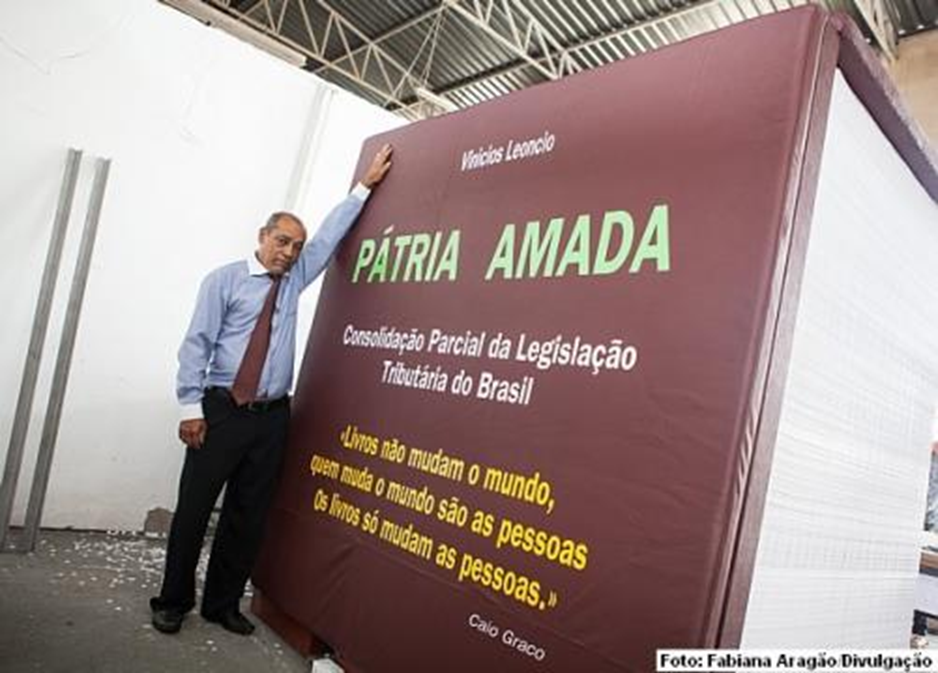
\includegraphics[width=0.5\linewidth]{Imagens/a1i1.png}
\end{figure}

\begin{itemize}
    \item Por que fazer reformas é tão difícil, mesmo quando se sabe que são essenciais? 
    \item Qual é a lógica da política? (a mesma econômica?)
\end{itemize}

\subsection{\textbf{Analisando uma situação}}
Quatro crianças querem comer cookies. Há duas formas possíveis de dispô-los:\begin{enumerate}
    \item Um grande jarro (\textbf{Bens comuns}) onde se encontram 40 cookies. Cada criança pode pegar o quanto quiser. As crianças podem fazer mais cookies, mas os novos  devem ir para o grande jarro 
    \item Cada criança terá um jarro particular(\textbf{Bens Privados}) contendo 10 cookies, e só poderá comer cookies de seu próprio jarro. Cada uma pode fazer mais cookies e colocar dentro de seu jarro.
    \item \begin{enumerate}
        \item Com o jarro pequeno, há incentivo para produção. Pode haver desperdício(caso exista um outro alimento a ser consumido, pode haver trocas, levando em consideração a utilidade de cada criança perante as suas preferências). Normalmente, devido a situações vistas normalmente, é a que garente um retorno melhor.
        \item Consumo/"distribuição" desigual. Possibilidade de organização/cooperação. Algo bem parecido com instituições informais, e normalmente não são alcançáveis.
    \end{enumerate}
\end{enumerate}

Considere as leis de pesca baleeira do século XIX (e abstraindo um pouco nossa ética ambientalista do século XXI...). Havia três regras possíveis
\begin{enumerate}
    \item Se um pescador atingir primeiro a baleia com seu arpão mas perdê-la, e se depois outro pescador conseguir matar a baleia, o primeiro não terá direito algum.
    \item O primeiro pescador terá direito à metade da baleia, mesmo que não tenha matado de fato.
    \item O primeiro pescador terá direito à baleia inteira, caso o seu arpão permaneça na baleia, mesmo que a corda tenha arrebentado e a baleia fugido.
\end{enumerate}

\subsection{\textbf{Esquema geral da disciplina}}
\begin{figure}[H]
    \centering
    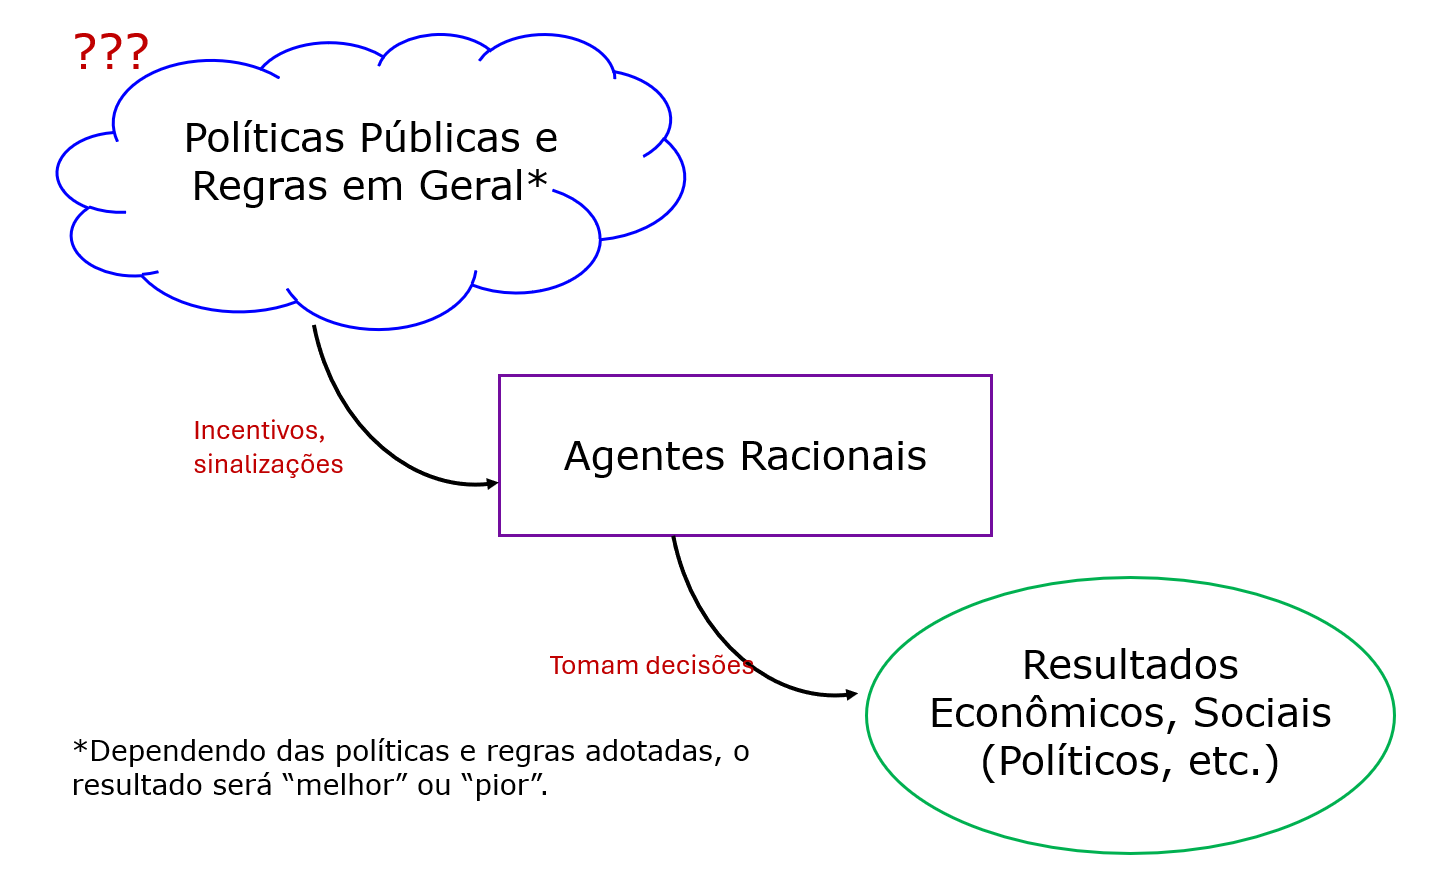
\includegraphics[width=0.75\linewidth]{Imagens/a1i2.png}
\end{figure}

\subsection{\textbf{Avaliações}}
\begin{itemize}
    \item Prova Intermediária(\textbf{PI}): 35\% na média final
    \item Prova Final(\textbf{PF}): 35\% na média final
    \item Estudo Dirigido 10\% na média final
    \item Trabalho Final 10\%
\end{itemize}

\subsection{\textbf{Vamos começar falando certo...}}
\textbf{Eficiência $\neq$ Justiça e Justiça $\neq$ Eficiência}

E nós NÃO VAMOS falar sobre Justiça aqui! (Por que???)

\section{\textbf{Economia Institucional - Parte 1}}
\subsection{\textbf{Da Economia Clássica}}
\begin{itemize}
    \item Ciência econômica como ciência da tomada de decisão ou comportamento humano.
    \item Agentes comportam-se basicamente pela maximização de utilidade sujeito a restrições e preferências. 
    \item Adoção de modelos para possibilitar a análise científica. 
    \item Assume racionalidade perfeita, informações perfeitas e ausência de custos de transação ou qualquer outro tipo de falhas de mercado.  
\end{itemize}

\subsubsection{\textbf{Mas}}
“Existem falhas de mercado a cada esquina...” (LY)\begin{itemize}
    \item Competição imperfeita;
    \item Externalidades;
    \item Bens Públicos;
    \item Informação Imperfeita;
    \item Custos de transação
    \item … enfim, Falhas de Mercado.
\end{itemize}

Ainda, os agentes humanos:\begin{itemize}
    \item têm capacidade cognitiva limitada; 
    \item Apresentam vieses de comportamento;
    \item São muito imperfeitos na tomada de decisão. 
\end{itemize}

\subsection{\textbf{Da Economia Clássica para a Nova Economia Institucional}}
A Nova Economia Institucional tem como diferencial:\begin{itemize}
    \item \textbf{Objeto de estudo}: as regras(leis, contratos,...) em vigor não são mais dadas, sua escolha e sua evolução ao longo do tempo são parte principal da análise.
    \item \textbf{Hipóteses adotadas}: racionalidade limitada(mas os agentes continuam racionais) (\textit{bounded rationality}) ao invés de perfeita, e existência de custos para trocas, ou custos de transação.
\end{itemize}

\subsection{\textbf{A Nova Economia Institucional (NEI) e Douglas North}}
\begin{figure}[H]
    \centering
    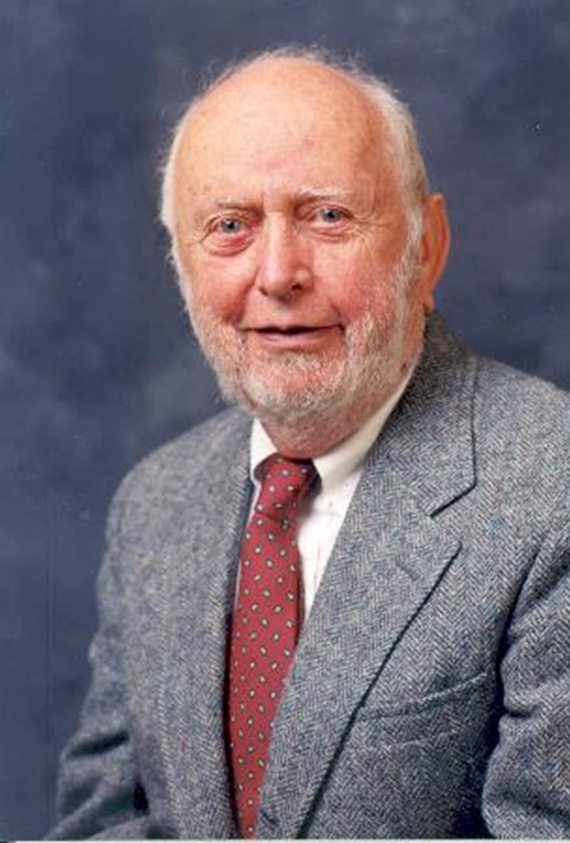
\includegraphics[width=0.5\linewidth]{Imagens/a2i1.png}
\end{figure}
Olhando sempre para dados empíricos, usando ferramentais, modernos(para a época), como é o caso de econometria, para tender entender como as coisas funcionam.

"\textbf{Instituições \textit{são as regras do jogo na sociedade}} ou, mais formalmente, são restrições humanamente criadas que moldam as interações humanas. Como consequência, elas estruturam os incentivos nas trocas humanas, sejam trocas políticas, sociais ou econômicas. Mudanças institucionais moldam a maneira como as sociedades desenvolvem-se ao longo do tempo e, portanto, são cruciais no entendimento das mudanças históricas” \textit{(Douglas North, 1990, p.3).}$\rightarrow$ Isso é uma definição formal, "positiva", no sentido que está é a definição. North definiu o que é uma instituição .

Instituições efetiva levam ao crescimento e desenvolvimento econômico: “a eficácia das instituições e sua garantia (\textit{enforcement}) determinam o nível dos custos de transação”; por sua vez, “os custos de transação são determinantes críticos do desempenho econômico” (1989, p. 803). Como consequência, \textbf{instituições efetivas são aquelas que aumentam os benefícios das soluções cooperativas [...], reduzem os custos de produção e os custos de transação de cada troca, de forma que os ganhos potenciais das trocas são auferidas}” \textit{(1991, p. 98)}. $\rightarrow$ Neste caso North definiu de forma normativa, implicando um certo viés do que as \textbf{Instituições} devem fazer serem \textbf{Instituições Eficientes}.

\subsubsection{\textbf{Uma outra definição de Instituições}}
"Intituições são \textbf{regras comumente conhecidas} usadas para estruturar situações de interação recorrentes tendo tais regras \textbf{mecanismo sansionador}

\subsection{\textbf{"Why Nations Fail"... E não o contrário}}
Um estudo empírico, feito em \textit{papers}, utilizando métodos econométricos sofisticados, realizaram um estudo histórico, visitando países, colônias e acompanharam o seu desenvolvimento com dados e chegaram a resultados quantitativos promissores sobre a influências de instituições sobre o sucesso e/ou fracasso das nações. 

\begin{figure}[H]
    \centering
    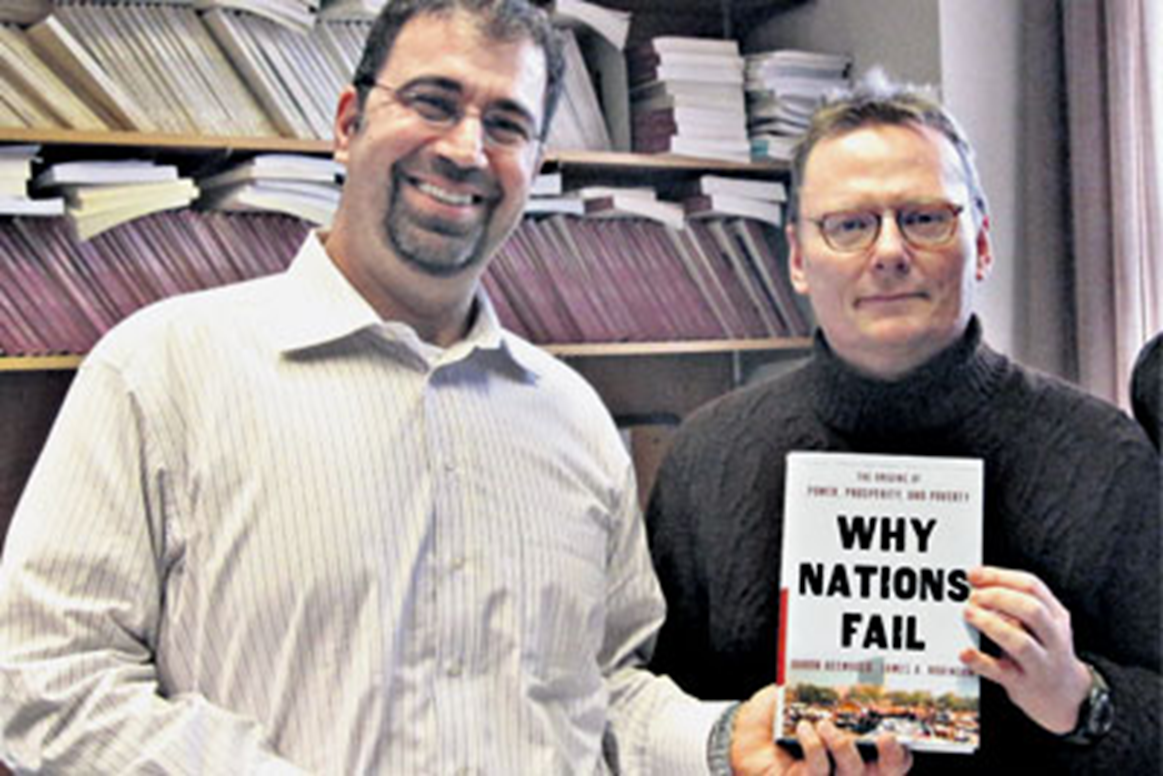
\includegraphics[width=0.5\linewidth]{Imagens/a2i2.png}
\end{figure}

\begin{figure}[H]
    \centering
    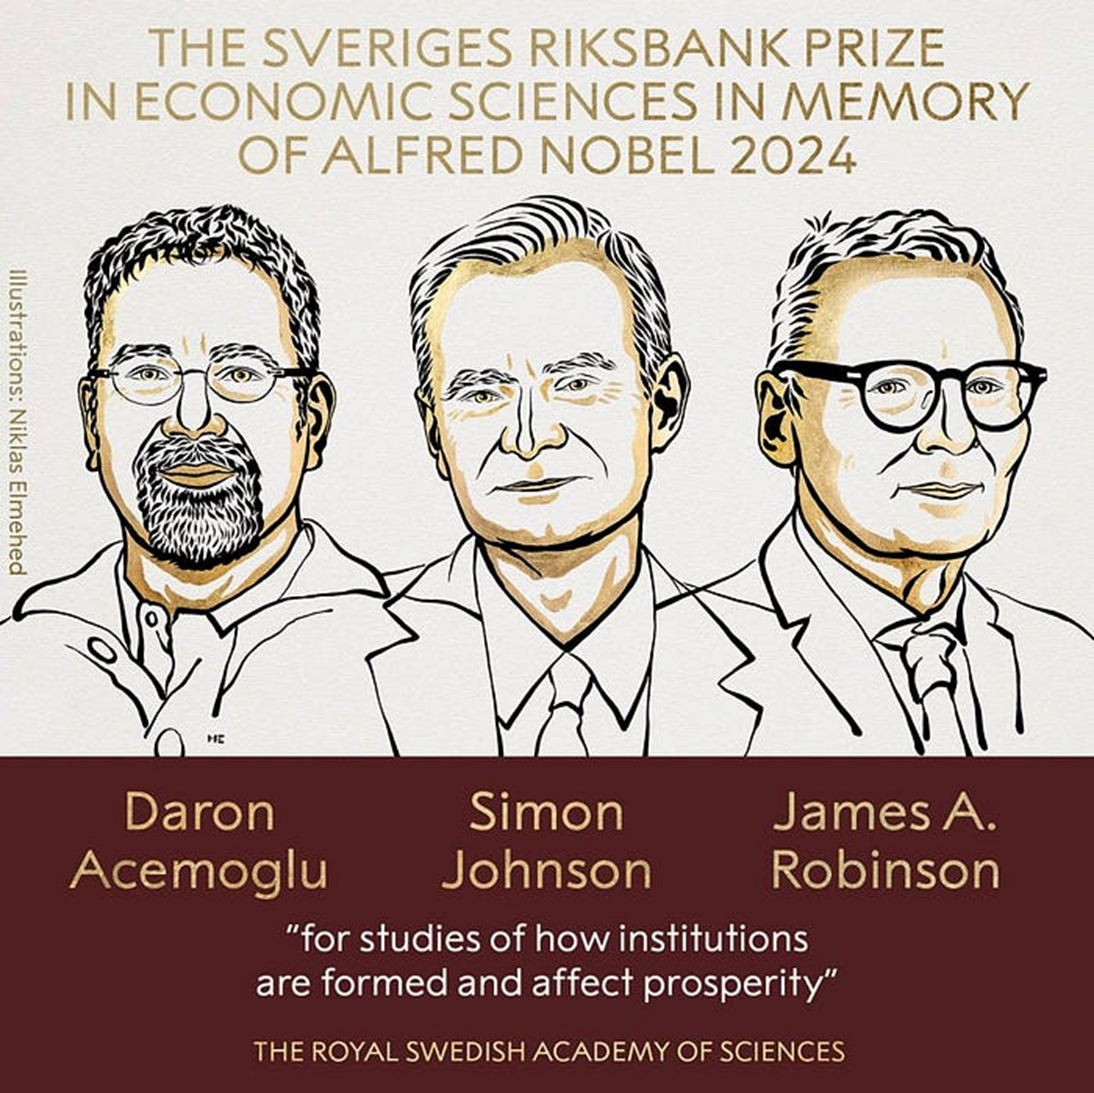
\includegraphics[width=0.5\linewidth]{Imagens/a2i3.png}
\end{figure}

Horizonte temporal da Era Neolítica ao ano de 2050, passando pelo Império Romano, Maias, tribos africanas, colonização latino-americana, países do leste europeu, EUA, Coreias, Argentina, Colômbia, China, etc... Por meio de descrições descobertas por meio de dados empíricos também.

\subsection{\textbf{História: Os irmãos Hwang}}
Junho de 1950; a Coreia é separada em Norte e Sul pelo Paralelo 38. O irmão de Hwang Pyong-Won, médico das forças armadas, é levado pelas tropas para o norte. Os irmãos são separados por 50 anos. 

Em 2000, Hwang Pyong-Won, agora um farmacêutico, tem a chance de se reencontrar com seu irmão, em um evento autorizado pelos dois governos. 

A diferença nos estilos de vida entre os dois irmãos é gritante. Além de não ter carro, telefone, casa própria, até o terno do irmão do norte era remendado: “É do governo, me emprestaram para esta visita”. Os outros visitantes do norte, invariavelmente, pediam dinheiro para seus parente do sul. O irmão de Hwang não quis: ”O governo vai tomar de mim depois, se você me der”. Ainda, a todo momento, ele olhava em volta suspeito, com medo que alguém o escutasse. Apesar de dizer que tinha uma boa vida, o irmão de Hwang estava mais pobre e raquítico do que ele havia imaginado...

Hoje, o padrão de vida dos sul-coreanos é similar aos dos sul-europeus, enquanto que o dos norte-coreanos é similar aos povos da África Sub-Saariana, ou seja, um décimo do padrão de seus familiares do sul. 

A diferença na expectativa de vida é de 10 anos. 

Diferenças na presença de propriedade privada, inovação e tecnologia, mercados, relações contratuais, educação de qualidade, entre outros, separam os dois lados do Paralelo 38.

“Nem a cultura, nem a geografia, ou a ignorância podem explicar os diferentes caminhos trilhados pela Coreia do Sul e do Norte. Temos que olhar para as \textbf{instituições [econômicas e políticas]} em busca de respostas” (p.73).

\subsection{\textbf{Acemoglu e Robinson (2012)}}
\begin{enumerate}
    \item A matriz das instituições, o crescimento sustentado e a dinâmica entre os quadrantes.
    \item “Cultura”.
    \item Qual é a relação entre centralização política e prosperidade econômica?
    \item A “Destruição Criativa”, relação com instituições e desenvolvimento econômico.
    \item Instituições que levam à prosperidade sempre.
\end{enumerate}

\subsection{\textbf{1. As Diferentes Instituições}}

Instituições Inclusivas e Instituições Extrativas.\begin{itemize}
    \item Não confundir as políticas com as econômicas! É uma distinção essencial que não podem ser confundidas. Mas ambas podem ser inclusivas e extrativistas, e existem suas combinações geram resultados.
\end{itemize}

Melhor:\begin{itemize} 
    \item Instituições Políticas Inclusivas e Não-Inclusivas;
    \item Instituições Econômicas Extrativas e Não-Extrativas.\begin{itemize}
        \item Instituições Econômicas Extrativas são consideradas \textbf{ruins}, pois sua função extrair renda(Colonização espanhola e portuguesa foi extrativista, ao contrário da colonização norte americana)
    \end{itemize}
\end{itemize}

As combinações possíveis (nossa matriz 2x2):\begin{itemize}
    \item Políticas não inclusivas (extrativas) x Econômicas extrativas.
    \item Políticas inclusivas x Econômicas extrativas.
    \item Políticas não inclusivas x Econômicas não-extrativas (inclusivas).
    \item Políticas inclusivas x Econômicas não-extrativas
\end{itemize}

\begin{figure}[H]
    \centering
    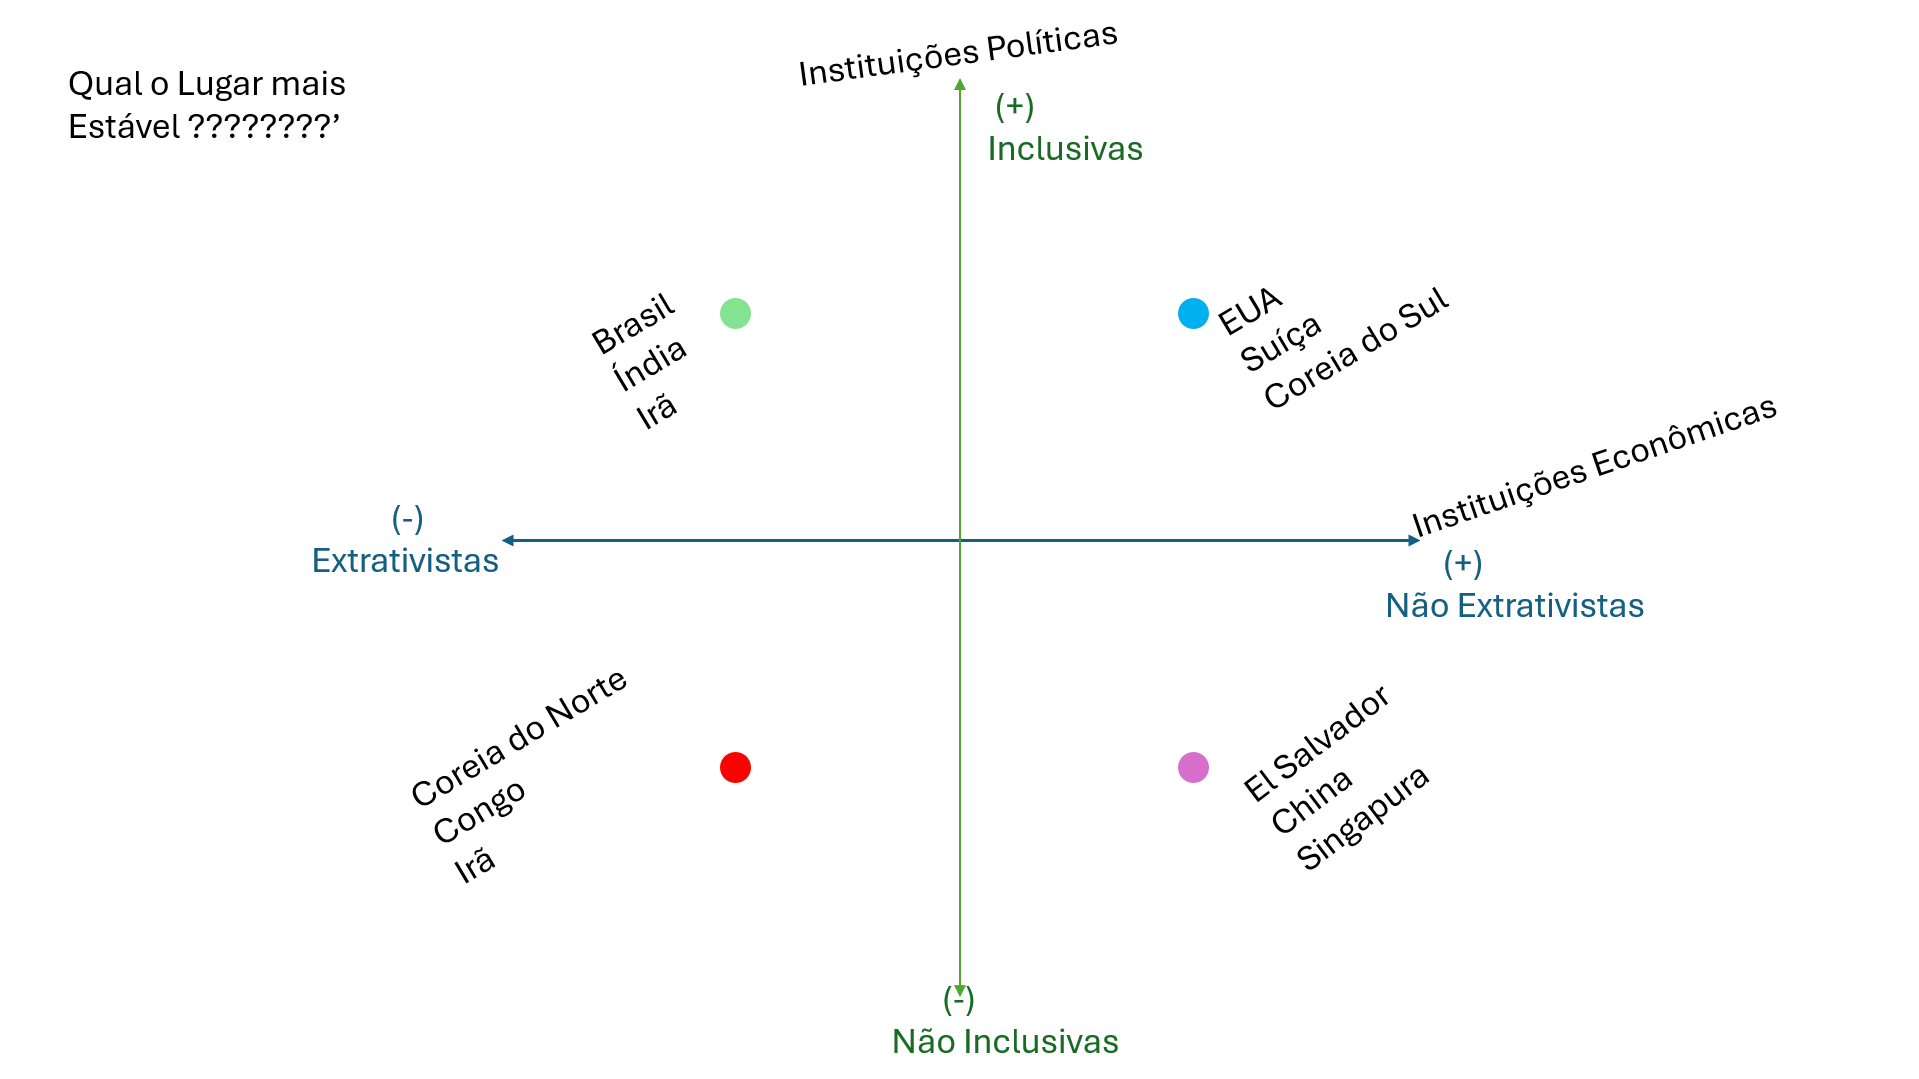
\includegraphics[width=0.5\linewidth]{Imagens/a3i1.png}
\end{figure}

\begin{table}[H]
\begin{tabular}{lll}
                                  & \textbf{Economia Extrativa} & \textbf{Economia Não Extrativas} \\
\textbf{Políticas Inclusivas}     & Dois                        & Um                               \\
\textbf{Políticas Não Inclusivas} & Três                        & Quatro                          
\end{tabular}
\end{table}


\subsubsection{\textbf{Instituições Políticas Não-Inclusivas com Econômicas Extrativas}}
\begin{figure}[H]
    \centering
    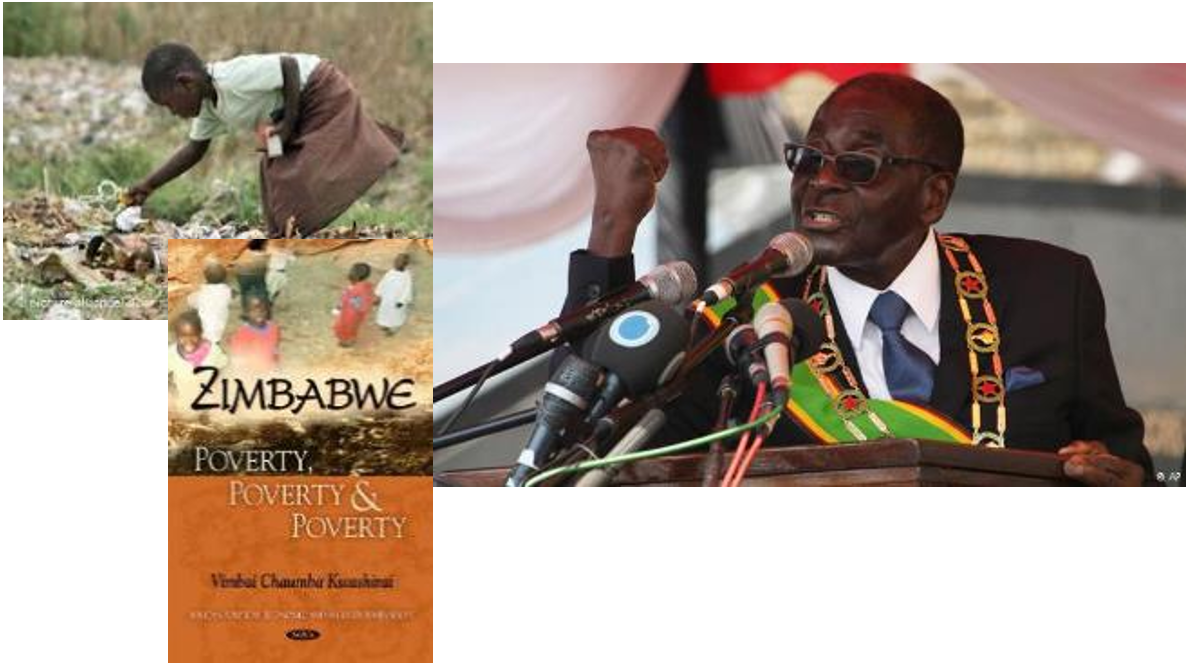
\includegraphics[width=0.5\linewidth]{Imagens/a2i4.png}
\end{figure}

\subsubsection{\textbf{Instituições Políticas Inclusivas com Econômicas Extrativas}}
Poderia ser o Brasil... \begin{itemize}
    \item Inclusão “falsa” ou “ineficaz”
    \item “Captura” das instituições econômicas por agentes políticos.
\end{itemize}

\subsubsection{\textbf{Instituições Políticas Não-Inclusivas com Econômicas Não-Extrativas}}
Existem?\begin{itemize}
    \item Sim!
\end{itemize}

\begin{figure}[H]
    \centering
    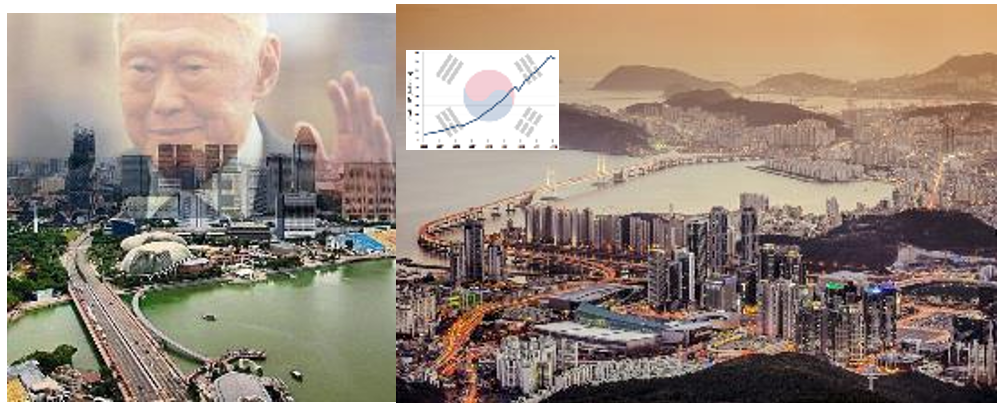
\includegraphics[width=0.5\linewidth]{Imagens/a2i5.png}
\end{figure}
\textbf{Mas geralmente é por um período limitado no tempo, não é equilíbrio estável!}

Algum nível de prosperidade econômica é intrínseco ao processo de centralização do Estado e de criação de \textit{law and order}.

Para que a prosperidade seja sustentável, as instituições econômicas precisam rapidamente passar pela transição para se tornarem não-extrativas, e as políticas, para se tornarem inclusivas.

É por isso que os autores apostam no fim iminente do grande crescimento chinês (último capítulo do livro).

\subsubsection{\textbf{Instituições Políticas Inclusivas com Econômicas Não-Extrativas}}

\begin{figure}[H]
    \centering
    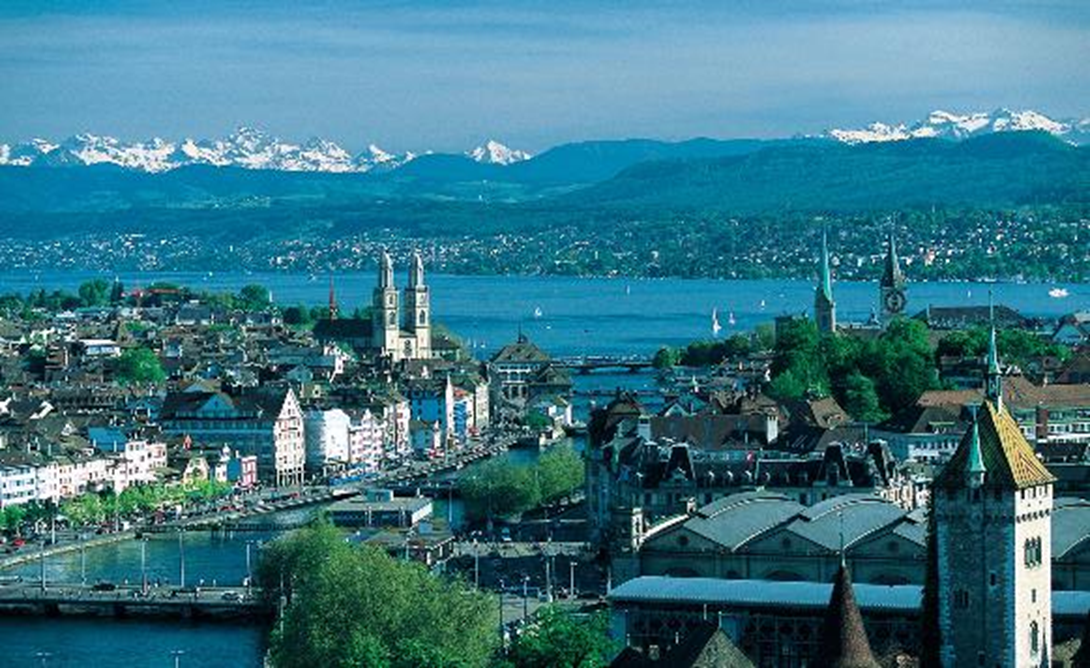
\includegraphics[width=0.5\linewidth]{Imagens/a2i6.png}
\end{figure}

\subsection{\textbf{“Cultura”}}
\begin{itemize}
    \item Muito cuidado com o termo (que pode significar múltiplas questões).
    \item Muito (mais) cuidado com o “fatalismo cultural”: povos de cultura idêntica chegam a resultados completamente diferentes em menos de uma geração (centenas de exemplos ao longo da história).
    \item Cultura é, no máximo, fator impactante, \textbf{mas não determinante}.
    \item (Dificuldade da teoria econômica em explicar a relação da “cultura” com a adoção de tipos de instituições.)
\end{itemize}

\subsection{\textbf{Centralização Política e Crescimento Econômico (qual é a relação?)}}
\begin{itemize}
    \item A centralização política mínima é necessária para o crescimento e desenvolvimento.\begin{itemize}
        \item “Lei e ordem” devem ser garantidos.
    \end{itemize}
    \item No entanto, a centralização política não pode gerar instituições políticas que não sejam inclusivas. 
    \item Deve haver uma rápida transição dos sistemas com instituições políticas não inclusivas com instituições econômicas não-extrativas para um sistema de instituições políticas inclusivas com instituições econômicas não-extrativas.\begin{itemize}
        \item Desenvolvimento e prosperidade sustentadas. 
    \end{itemize}
    \item Previsão para o futuro da China. 
\end{itemize}

\subsection{\textbf{“Destruição Criativa” de Schumpeter(p. 86, Cap. 3)}}
\begin{figure}[H]
    \centering
    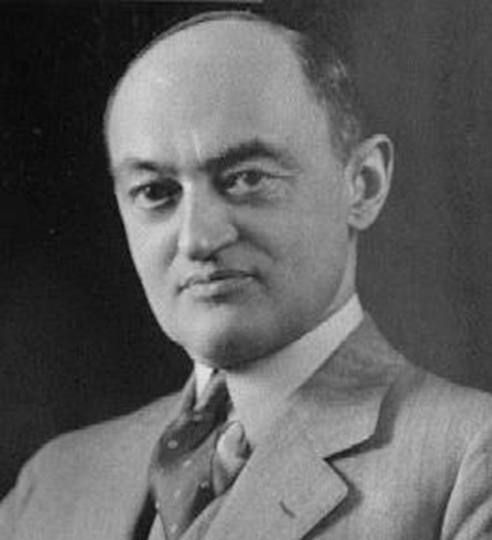
\includegraphics[width=0.5\linewidth]{Imagens/a2i7.png}
\end{figure}
“O Capitalismo [...] é por natureza uma forma ou método de mudança econômica e nunca é, nem pode ser estacionário [...] O impulso fundamental que define e que mantem o motor capitalista em ação vem dos novos bens de consumo, os novos métodos de produção ou transporte, os novos mercados, as novas formas de organização industrial que a empresa capitalista cria [...] A abertura de novos mercados, estrangeiros ou domésticos, e o desenvolvimento organizacional [...] ilustram o processo de mutação industrial que revoluciona constantemente a estrutura econômica \textbf{de dentro}, destruindo incessantemente o ‘antigo’, e incessantemente criando um ‘novo’. Este processo de \textbf{Destruição Criativa }é o fato essencial do Capitalismo. É nisso no que consiste o Capitalismo e no cada preocupação dos capitalistas deveria consistir. [... O Capitalismo requer] a tempestade permanente da Destruição Criativa”. \textit{Capitalism, Socialism and Democracy (1942)}

\subsection{\textbf{Quais Instituições Importam para a Prosperidade?}}
As instituições são resultados da evolução histórica, cultural, social de cada nação, por isso tem suas peculiaridades nacionais.

No entanto, olhando para a evolução da humanidade, é possível perceber que há grandes grupos de instituições que todos as nações que se desenvolveram de maneira sustentável adotaram:\begin{itemize}
    \item Respeito à propriedade privada;
    \item Garantia do cumprimento dos contratos;
    \item Sistema judicial independente e eficiente;
    \item Liberdade de escolha (“reconhecer o talento que as pessoas têm...”);
    \item Democracia;
    \item Etc... 
\end{itemize}

\subsection{\textbf{Principal mensagem da economia institucional... E deste Capítulo}}
A hipótese central e básica da Economia Institucional (NEI) é que o crescimento e desenvolvimento de povos e nações é moldado de maneira decisiva pelas instituições prevalecentes. 

(O que são instituições?)

A Economia Clássica têm negligenciado o estudo das instituições (apesar de cada vez menos, e apesar de não ignorar totalmente). 

Boas teorias econômicas devem ser testáveis (falseáveis) empiricamente.

Já aprendemos muito com a teoria da NEI (e sobretudo de Acemoglu e coautores) que, por enquanto, está sendo corroborada empiricamente (mas ainda está sob verificação).

No entanto, a materialização em políticas públicas que sejam baseadas nesses aprendizados é outra estória... \begin{itemize}
    \item (A vontade e a ação política nem sempre é guiada pela racionalidade econômica...) 
\end{itemize}

\newpage
\section{\textbf{Direitos de Propriedade-Parte 1}}
\subsection{\textbf{“Destruição Criativa” de Schumpeter(p. 86, Cap. 3)}}
\begin{figure}[H]
    \centering
    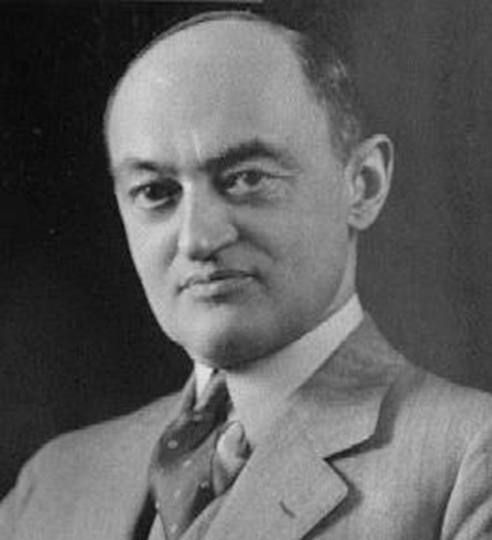
\includegraphics[width=0.5\linewidth]{Imagens/a2i7.png}
\end{figure}
“O Capitalismo [...] é por natureza uma forma ou método de mudança econômica e nunca é, nem pode ser estacionário [...] O impulso fundamental que define e que mantem o motor capitalista em ação vem dos novos bens de consumo, os novos métodos de produção ou transporte, os novos mercados, as novas formas de organização industrial que a empresa capitalista cria [...] A abertura de novos mercados, estrangeiros ou domésticos, e o desenvolvimento organizacional [...] ilustram o processo de mutação industrial que revoluciona constantemente a estrutura econômica \textbf{de dentro}, destruindo incessantemente o ‘antigo’, e incessantemente criando um ‘novo’. Este processo de \textbf{Destruição Criativa }é o fato essencial do Capitalismo. É nisso no que consiste o Capitalismo e no cada preocupação dos capitalistas deveria consistir. [... O Capitalismo requer] a tempestade permanente da Destruição Criativa”. \textit{Capitalism, Socialism and Democracy (1942)}

O conceito de seleção natural, de Charles Darwin, vem agora para a economia.

\subsection{\textbf{Quais Instituições Importam para a Prosperidade?}}
As instituições são resultados da evolução histórica, cultural, social de cada nação, por isso tem suas peculiaridades nacionais.

No entanto, olhando para a evolução da humanidade, é possível perceber que há \textbf{grandes grupos de instituições} que todos as nações que se desenvolveram de maneira sustentável adotaram:\begin{itemize}
    \item Respeito à propriedade privada;
    \item Garantia do cumprimento dos contratos;
    \item Sistema judicial independente e eficiente;
    \item Liberdade de escolha (“reconhecer o talento que as pessoas têm...”);
    \item Democracia;
    \item Etc... 
\end{itemize}

\subsubsection{\textbf{Principal mensagem da economia institucional... }}

A hipótese e a conclusão central e básica da Economia Institucional (NEI) é que \textit{\textbf{o crescimento e desenvolvimento de povos e nações é moldado de maneira decisiva pelas instituições prevalecentes.}}

\subsection{\textbf{Economia dos Direitos de Propriedade}}
\begin{figure}[H]
    \centering
    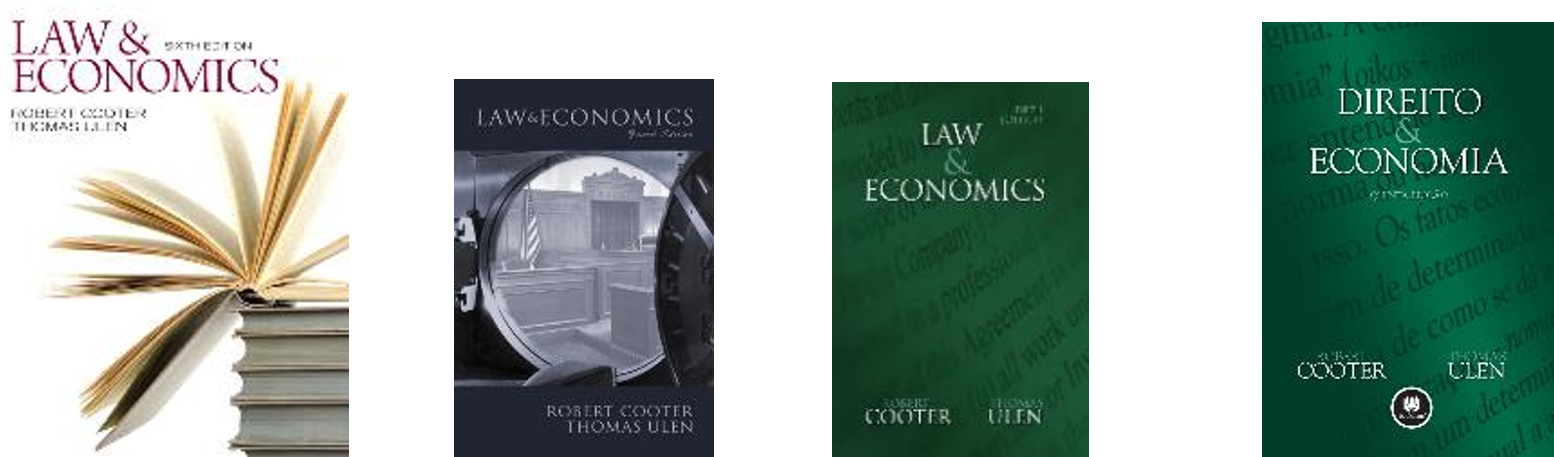
\includegraphics[width=0.5\linewidth]{Imagens/a4i1.png}
\end{figure}

\subsubsection{\textbf{Alguns casos...}}
\begin{figure}[H]
    \centering
    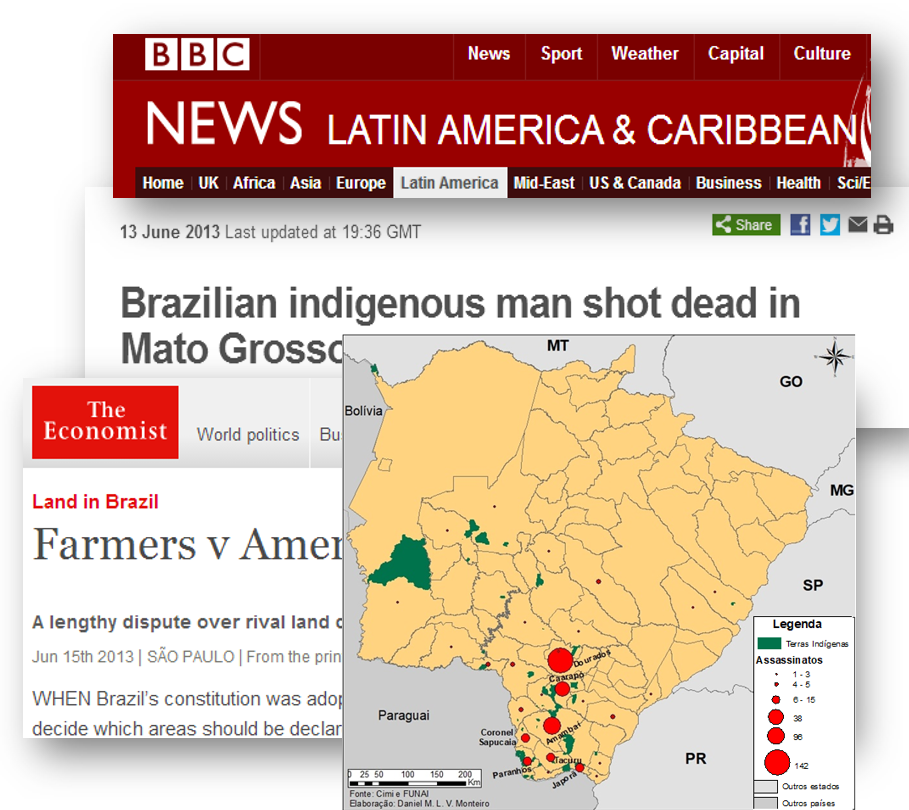
\includegraphics[width=0.5\linewidth]{Imagens/a4i2.png}
\end{figure}

\begin{figure}[H]
    \centering
    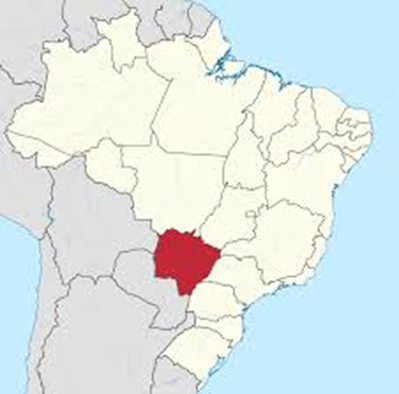
\includegraphics[width=0.5\linewidth]{Imagens/a4i3.png}
\end{figure}

O Mato Grosso do Sul delimita uma região de grande relevância econômica para o agronegócio brasileiro, principalmente na produção e exportação de grãos e carne bovina.

Também concentra a segunda maior população indígena do país.

A maioria das terras em disputa foi adquirida por boa fé, embora concedida a povos indígenas nativos, seguindo a legislação brasileira, inclusive a Constituição Federal de 1988.

\begin{figure}[H]
    \centering
    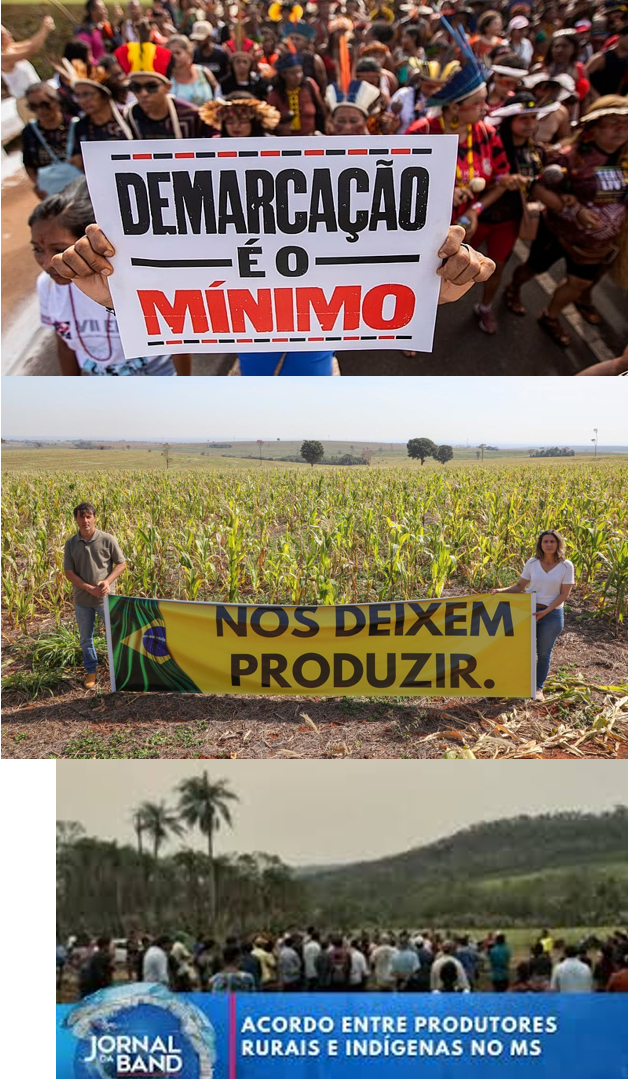
\includegraphics[width=0.5\linewidth]{Imagens/a4i4.png}
\end{figure}

\textbf{Produtores rurais x indígenas}
E o imbróglio continua...
A decisão, em agosto de 2023 foi...
Mas não acabou aí! 

\subsection{\textbf{Caso 1: Produtores rurais x indígenas}}
\textbf{Pergunta}: a quem deve caber o direito de propriedade destas terras? (Ou, o que precisamos saber para responder a esta pergunta?)

\subsection{\textbf{Alguns casos... }}
\begin{figure}[H]
    \centering
    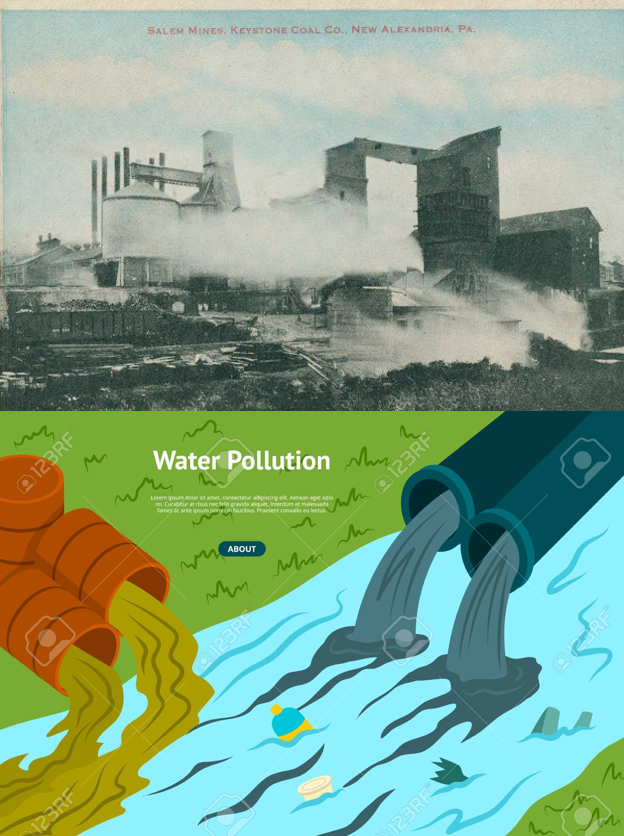
\includegraphics[width=0.5\linewidth]{Imagens/a4i5.png}
\end{figure}
Em 1868, a Sra. Eliza Sanderson comprou um pedaço de terra nas margens do Rio Meadow Brook em Scranton, Pensilvânia (EUA). Dois anos depois, ela terminou a construção de uma casa na propriedade, bem como barragens e tubulações para levar água do riacho para uma lagoa, uma cisterna e uma fonte. Ao escolher este local, a Sra. Sanderson foi atraída pelo fluxo e pureza da água, tanto para o uso doméstico como para fins comerciais.

Quase simultaneamente, a Pennsylvannia Coal Company abriu uma mina de carvão três milhas a montante (acima no rio). Com suas operações, a empresa poluiu tanto o rio que tornou a lagoa da Sra. Sanderson inutilizável para fins de criação de peixes ou outra atividade comercial e todo o sistema de tubos foi corroído e destruído. Muito de seu investimento na propriedade foi completamente perdido. Ela processou a empresa.

\textbf{Pergunta}: a quem deve caber o direito de propriedade destas terras? (Ou, o que precisamos saber para responder a esta pergunta?)

Mas isso é problema de definição de direitos de propriedade?

Coase (1960): direitos de propriedade fazem parte do conjunto de fatores de produção (talvez o mais importante) de qualquer empresa/organização. 

O valor de um “papel”...

Os informais devem ser protegidos? 

[“De Favelado a Dono de Casa Própria – Revista Época, 24/09/2009]

Caso semelhante já discutido em aula: Lei de Usucapião.

Pergunta para o Caso 2: Uma lei como o “Papel Passado” é uma lei desejável? Quais razões a AED daria?

\subsection{\textbf{Propriedade: diferentes definições }}
\textbf{Questões Filosóficas}\begin{itemize}
    \item Utilitarismo (Bentham): A propriedade é base sobre a qual se obtém \textbf{expectativas de benefícios} dos bens que temos posse. 
    \item Justiça (Aristóteles): O sistema de propriedade privada pode ser usado para gerar uma sociedade mais ou menos \textbf{igualitária}.
\end{itemize}

E pra quê saber isso???

\subsection{\textbf{Análise Econômica dos Direitos de Propriedade}}
\begin{figure}[H]
    \centering
    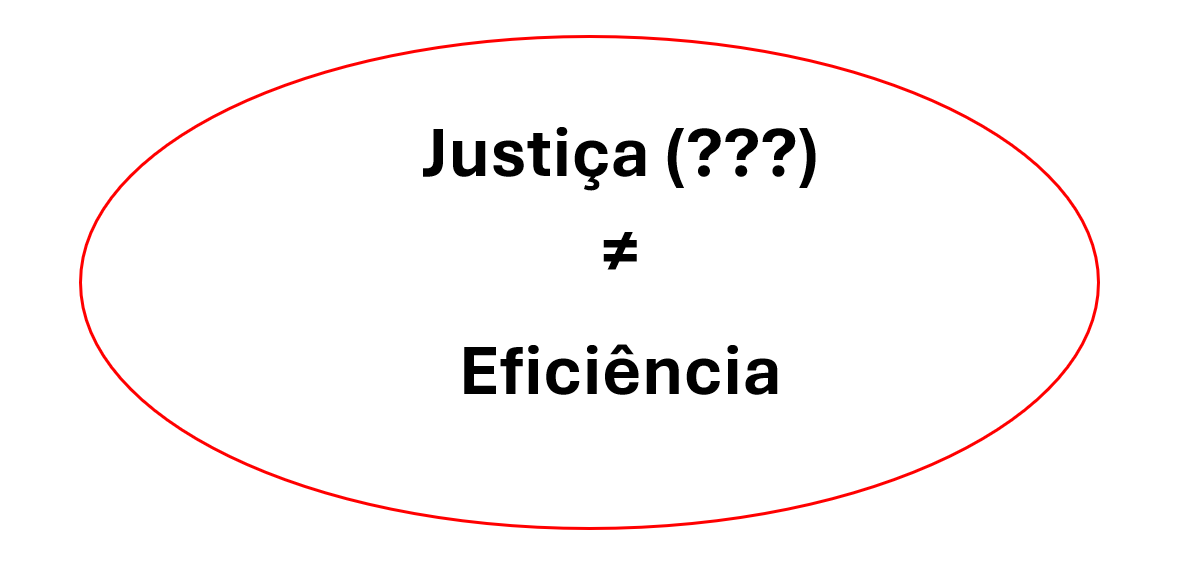
\includegraphics[width=0.5\linewidth]{Imagens/a4i6.png}
\end{figure}

max dos benefícios líquidos das partes envolvidas

\subsection{\textbf{Um Conceito e uma Diferenciação Importante}}
Eficiência (melhora) de Pareto(\textit{Situação em que eu não consigo melhorar minha solução sem prejudicar a do outro}) x Eficiência \textbf{(melhora) de Kaldor-Hicks}(\textit{ganhos que sejam maiores que perdas})

No limite a eficiência de Kaldor-Hicks, via transferência de ganhos ao ponto que supere as perdas, a eficiência se torna de Pareto.

\subsection{\textbf{Direitos de Propriedade}}
Quem define os direitos de propriedade?\begin{itemize}
    \item As leis, as instituições legais, ou as regras sociais (informais).
\end{itemize}

As leis garantem, necessariamente, eficiência?\begin{itemize}
    \item Não!  (Por que não?)
    \item Ex.: Eficiência x Igualitarismo como objetivos de políticas.
\end{itemize}

\subsection{\textbf{Esquema Geral da AED}}
\begin{figure}[H]
    \centering
    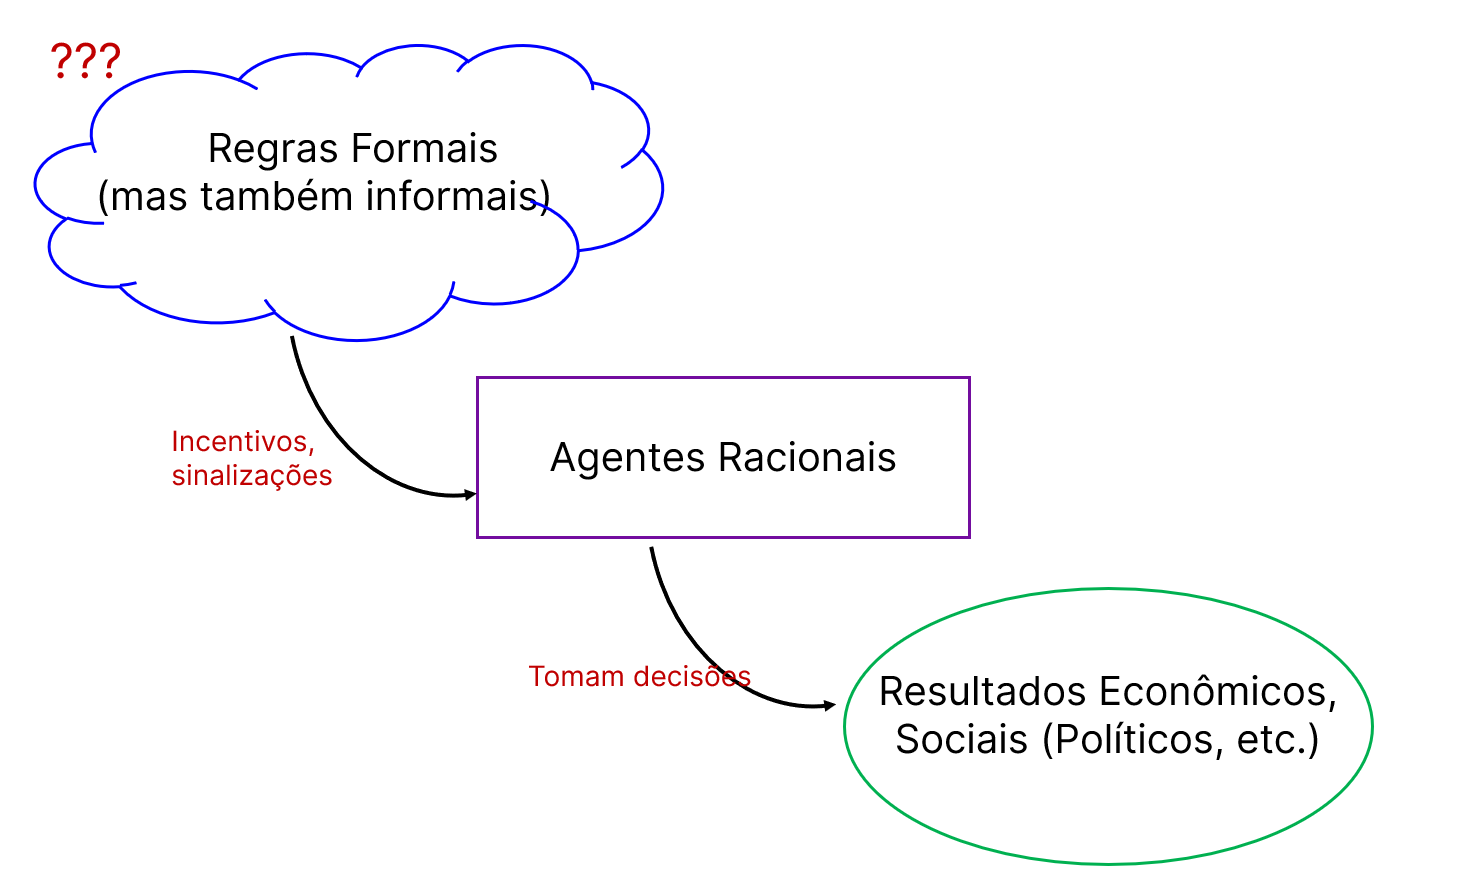
\includegraphics[width=0.5\linewidth]{Imagens/a4i7.png}
\end{figure}

\subsection{\textbf{A Constituição Federal do Brasil}}
Art. 5º Todos são iguais perante a lei, sem distinção de qualquer natureza, garantindo-se aos brasileiros e aos estrangeiros residentes no País a inviolabilidade do direito à vida, à liberdade, à igualdade, à segurança e à propriedade, nos termos seguintes: (...) \begin{itemize}
	\item XXII - é garantido o direito de propriedade;\textbf{(Concede)}
	\item XXIII - a propriedade atenderá a sua função social (...)\textbf{(Limita)}
	\item XXV - no caso de iminente perigo público, a autoridade competente poderá usar de propriedade particular, assegurada ao proprietário indenização ulterior, se houver dano (...)\textbf{(Limita)}
\end{itemize}

As leis estão garantindo a eficiência(e qual a eficiência)? 

\subsection{\textbf{Direitos de Propriedade e Eficiência}}
Análise(afirmação) positiva(ela vem de uma observação) para uma afirmação normativa(vem de uma "opinião"). Usamos da econometria para ver relações entre as variáveis(análise positiva) e tirar disso relações causais(afirmação normativa).

Direitos de propriedade bem-definidos farão com que o recurso seja alocado ao uso que gere mais bem-estar (eficiência). Isso é uma frase bem normativa.

Exemplo:\begin{itemize} 
    \item firma informal que se torna formal; 
    \item invenção sendo feita por aquele que tem capacidade de produzir o conhecimento;
    \item direito de propriedade por aquele que faz uso que maximiza o benefícios gerado para a sociedade;
    \item terreno ocupado ilegalmente que passa a ser reconhecido.
\end{itemize}

\subsection{\textbf{O conceito legal de “propriedade''}}
Um conjunto de direitos que descreve o que as pessoas \textbf{podem ou não podem fazer} com os recursos que possuem. 

\textbf{Quem tem uma propriedade não quer dizer que pode fazer o que quiser com ela}...\begin{itemize}
    \item Voltando ao caso da Sra. Sanderson...
    \item Voltando aos produtores rurais do MS (ou RR, ou SP...)
\end{itemize}

Estes direitos são mutáveis através do tempo e do espaço, logo possíveis soluções/argumentos econômicos pode não ser mais válidos.\begin{itemize}
    \item Criador de porcos em Bragança Paulista. Temos que olhar em ambos os períodos de tempo(hoje e 30 anos atrás) e os ganhos e perdas desses períodos para ver se hoje é eficiente.
    \item \begin{table}[H]
\begin{tabular}{lllll}
\textbf{Fazenda}       & \textit{Ganhos}                                                                      & \textbf{Resultado}           & \textit{Perdas}                        & \textbf{Resultado} \\
\textit{30 anos atrás} & \begin{tabular}[c]{@{}l@{}}Emprego; \\ Consumo de Comida\end{tabular}                & \textgreater{}\textgreater{} & "Ambientais"                           & Eficiente          \\
\textit{Hoje}          & \begin{tabular}[c]{@{}l@{}}Emprego; \\ \(\downarrow\) Consumo de Comida\end{tabular} & \textless{}\textless{}       & "\(\uparrow\) Ganho Relativo Ambiente" & Inificente        
\end{tabular}
\end{table}
\end{itemize}

\subsection{\textbf{Custos de Transação}}
Custos de transação são custos necessários para a efetivação das trocas. 

Os três passos da troca exigem custos específicos:\begin{itemize}
    \item custos de procura (bens únicos x bens padronizados)
    \item custos de barganha (informação pública x informação privada)
    \item custos de enforcement (imediato x longo prazo)
\end{itemize}

Custos de Transação\begin{enumerate}
    \item Comprar um pé de alface.
    \item Comprar um apartamento.
    \item Abrir uma franquia do MacDonald’s.
    \item Abrir uma franquia do Chipotle.
    \item Abrir legalmente uma microempresa de vestuário na Nova Zelândia.
    \item Abrir legalmente uma microempresa de vestuário no Bom Retiro.
    \item Comprar um carro novo.
    \item Comprar um carro usado.
    \item Casar.
    \item Encontrar um colega numa turma desconhecida para fazer um trabalho valendo 5\% da nota.
    \item Obs.: Dá para medir empiricamente custos de transação?
\end{enumerate}

\subsubsection{\textbf{(“intrínsecos” à transação)}}
\begin{figure}[H]
    \centering
    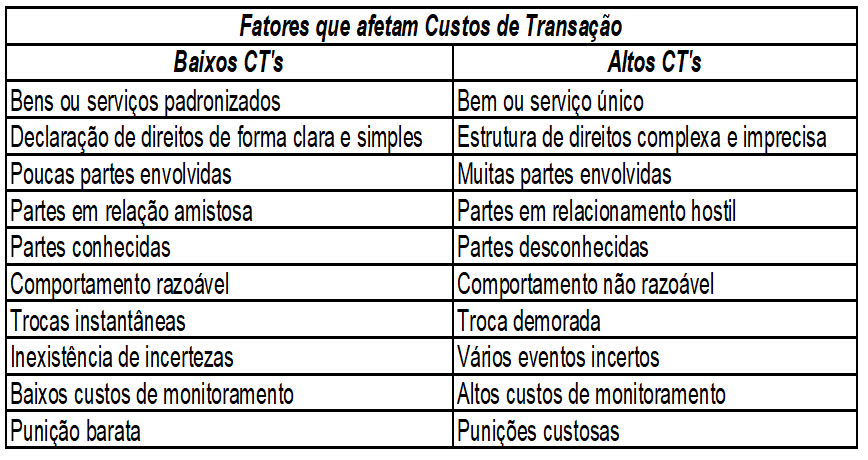
\includegraphics[width=0.7\linewidth]{Imagens/a5i1.png}
\end{figure}

As “leis” e os custos de transação: qual é a relação entre eles?

\begin{figure}[H]
    \centering
    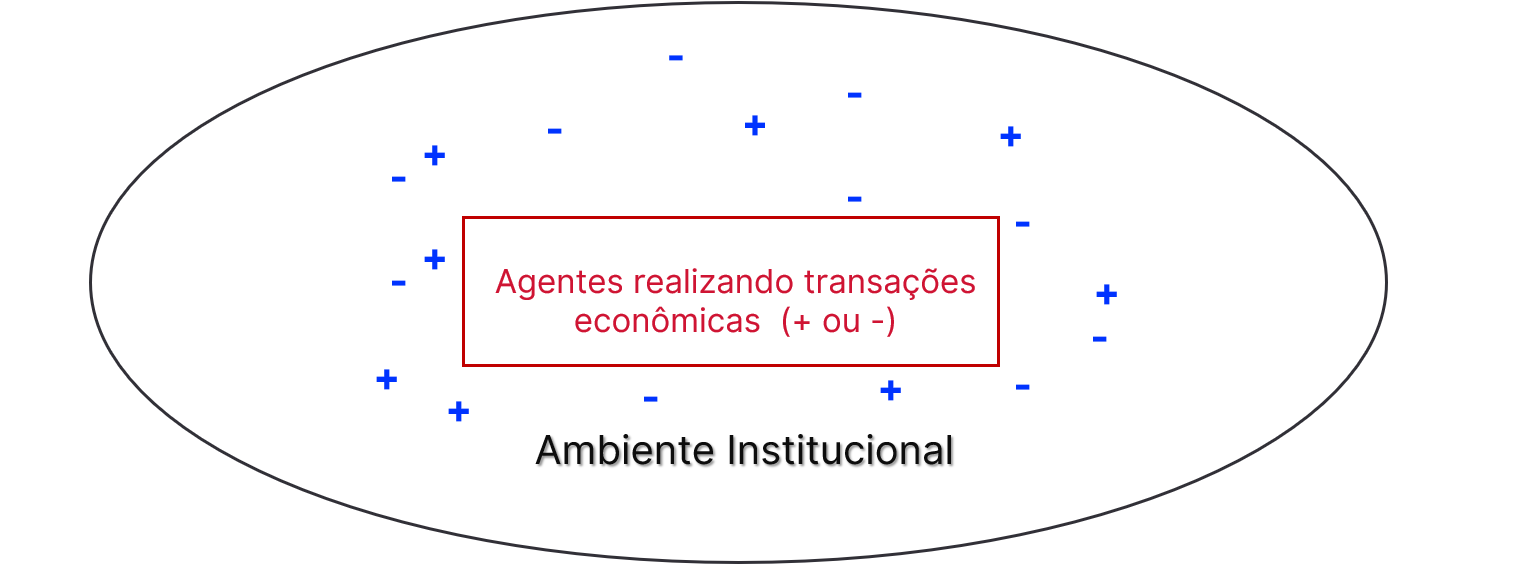
\includegraphics[width=0.75\linewidth]{Imagens/a5i2.png}
\end{figure}
O que os agentes irão fazer se os custos de transação extrínsecos forem muito altos no ambiente institucional? 
\textbf{FOCARÃO EM TRANSAÇÕES DE BAIXOS CUSTOS, OU SEJA, DE BAIXO VALOR!}
\newpage
\section{\textbf{Direitos de Propriedade-Parte 2}}
\subsection{\textbf{Teorema de Coase}}
Quando as partes barganham (negociar) de forma cooperativa, a alocação legal de direitos não importa. O uso dos recursos será eficiente, independente da lei.

Do contrário, se a lei é seguida de forma não-cooperativa pelas partes, a alocação legal de direitos tem impactos sobre a eficiência.

\subsubsection{\textbf{Em outras palavras}}
Quando os custos de transação são nulos (ou negligenciáveis) as partes barganham de forma cooperativa e a alocação legal de direitos não importa. O uso dos recursos será eficiente, independente da lei.
Do contrário, se os custos de transação forem altos, a alocação legal de direitos tem impactos sobre a eficiência. 
\subsection{\textbf{Coase (1960): Sturges vs Bridgman}}
Qual é a transação possível de ser feita em questão?

Qual seria a valoração das partes c.r.a. esta transação?

Como Coase avalia, usando o exercício que ficou conhecido como Teorema de Coase?

Uma solução cooperativa possível (assumindo-se certos valores):

O médico abandonaria seu direito se o dono da confeitaria pagasse um valor que cobrisse sua perda de renda devido ao barulho da confeitaria.

O confeiteiro estaria satisfeito em pagar este valor se ele fosse menor do que o quanto seria necessário para ele mudar para outra localidade ou comprar novos equipamentos.

\begin{table}[H]
\centering
\resizebox{\textwidth}{!}{ % Ajusta a tabela para caber na largura da página
\begin{tabular}{|c|c|c|c|c|c|c|}
\hline
\textbf{\(y=f(k,l,t,Direito)\)} & \textit{Com Barulho} & \textit{Sem barulho} & \textit{\begin{tabular}[c]{@{}c@{}}Barganha com \\ Médico\end{tabular}} & \textit{\begin{tabular}[c]{@{}c@{}}Filtro Acústico\\ (Custo 100)\end{tabular}} & \textit{\begin{tabular}[c]{@{}c@{}}Filtro Acústico\\ (Custo 100)\end{tabular}} & \textit{\begin{tabular}[c]{@{}c@{}}Filtro Acústico\\ (Custo 100)\end{tabular}} \\ \hline
\textit{Confeiteiro}            & 1000                 & 0                    & 299                                                                     & 950                                                                            & 900                                                                            & 1000                                                                           \\ \hline
\textit{Hoje}                   & 0                    & 700                  & 701                                                                     & 650                                                                            & 700                                                                            & 600                                                                            \\ \hline
\textit{\textbf{"TODO"}}        & 1000                 & 700                  & 100                                                                     & 1600                                                                           & 1600                                                                           & 1600                                                                           \\ \hline
\end{tabular}
}
\end{table}

Aqui vemos que caso o tribunal decida quem será beneficiado, o ganho final é de 1000 unidades monetárias. Mas vemos que caso as partes decidam entre elas firmar um acordo de compra de um equipamento de isolamento sonoro, temos que o ganho moetário final a ser atingido é maior 

\subsection{\textbf{Análise Positiva x Análise Normativa}}


\subsection{\textbf{Teorema de Coase}}

Quando os custos de transação são ou negligenciáveis as partes barganham de forma cooperativa e a alocação legal de direitos não importa. O uso dos recursos será eficiente, independente da lei.

Do contrário, se os custos de transação forem altos, a alocação legal de direitos tem impactos sobre a eficiência. 

\subsection{\textbf{O que deveria ser feito?}}
\textbf{Teorema Normativo de Coase: }
“Estruture a lei de modo a remover os impedimentos aos acordos privados”. 

Ou seja, a lei deveria reduzir os custos de transação para as barganhas privadas. 

\textbf{Teorema Normativo de Hobbes:}
“Estruture a lei de modo a minimizar o prejuízo causado por fracassos em acordos privados”.

Ou seja, a lei deveria resolver os conflitos da maneira mais eficiente – aquela resolução que teria surgido da barganha privada. 

\subsection{\textbf{Teorema de Coase Normativo}}
Se os custos de transação são baixos tudo o que importa é que os direitos sejam bem definidos e os resultados legais sejam de fácil previsão.

Quando os custos de transação são tão altos que se torna impossível o rearranjo das leis, as cortes influenciam diretamente o resultado econômico. 

\textbf{As cortes neste caso, precisam entender as consequências econômicas de suas decisões.}

Então… Para aumentar a eficiência e minimizar os danos, a lei \textbf{deveria}… \begin{itemize}
    \item …estabelecer os direitos de propriedade de maneira clara (ex ante);
    \item ...reduzir ao máximo, sempre que possível, os custos de transação para a negociação cooperativa;
    \item …alocar os direitos de propriedade para a parte que mais valoriza tais direitos, ou garantir que os ganhos sejam maiores do que as perdas (ex post).
    \item OU SEJA: “simular” o resultado que teria sido alcançado caso as partes tivessem negociado cooperativamente.  
    \item OU SEJA, garantir a Eficiência de Kaldor-Hicks.
\end{itemize}

\subsection{\textbf{Racionalidade do Teorema de Coase}}
Se os custos de transação são negligenciáveis, não importa a quem a lei favorece, o resultado eficiente será sempre eficiente.
Sem uma decisão cooperativa, o conflito precisaria ser resolvido pela lei, por exemplo, juízes.

\textbf{Ambas partes causam danos. (reciprocidade)}

O que os juízes decidem não é o que deve ser feito por quem, mas somente quem tem o direito de fazer o quê.

\textbf{Se transações são livres no mercado, então, é sempre possível modificar a alocação inicial ou legal de direitos.}

\subsection{\textbf{Contribuições de Coase}}
O direito de usar os recursos e a propriedade também faz parte dos fatores de produção de um agente econômico.

A pessoa que tem o direito de propriedade sobre uma terra tem na verdade, uma lista de direitos que descrevem as ações que pode tomar.

Se fatores de produção são considerados direitos de se exercer algo, então, o \textbf{direito de se causar um dano a alguém} (por meio da poluição, destruição do plantio, etc) \textbf{também é um fator de produção.}
\newpage
\section{\textbf{Direitos de Propriedade Intelectual}}
O que aprendemos até agora sobre Direitos de Propriedade?\begin{itemize}
    \item Direitos de Propriedade seguros e bem definidos são boas instituições que garantem prosperidade para pessoas e países. 
    \item Teorema de Coase (positivo): Quando as partes barganham (negociar) de forma cooperativa, a alocação legal de direitos não importa. O uso dos recursos será eficiente, independente da lei. Do contrário, se a lei é seguida de forma não-cooperativa pelas partes, a alocação legal de direitos tem impactos sobre a eficiência.
    \item Teorema de Coase normativo: A lei \textbf{deveria} reduzir os obstáculos às barganhas privadas cooperativas.
    \item Então, a conclusão
    \item Mas
\end{itemize}

\subsection{\textbf{A barganha privada não funciona}}
Algumas \textbf{falhas de mercado}, quando em grandes dimensões, dificultam muito/impedem o surgimento de direitos de propriedade de forma cooperativa:\begin{itemize}
    \item \textbf{Externalidades} externalidade negativa é um outro nome para custo social.
    \item \textbf{Bens públicos}
    \item \textbf{Monopólios naturais}
    \item Assimetria de informações
    \item Etc.
\end{itemize}

A informação é um típico exemplo de bem cujo direito de propriedade é mal-definido e, portanto, tem mercado deficiente:\begin{itemize}
    \item Informação é um \textbf{bem-público}: não-excludente(), não rival(eu consumir algo não empedi outra pessoa de consumir esse mesmo bem, dado que ele não chegou a exaustão).
    \item Informação gera \textbf{externalidades}.
\end{itemize}


\subsection{\textbf{Que tipo de bem é a Informação? (científica, artística, comercial, etc.)}}
Problema da \textbf{credibilidade}: compradores não podem avaliar com certeza o valor da informação até o momento em que a obtém. Quando a obtém, não tem mais incentivo para pagar por ela.

Outro problema: \textbf{impossibilidade de apropriação}.

Informação tem \textbf{custo muito alto de produção e muito baixo de transmissão. } \begin{itemize}
    \item Estima-se que custe , em média, \$ 900 milhões de dólares para desenvolver um novo medicamento (Salama e Benoliel).
\end{itemize}

Resultado: o mercado privado de informação tende a suprir informação em quantidade aquém do eficiente econômico. 

Estado precisa intervir no mercado de informações (produção, subsídio, proteção, etc.). 

\subsection{\textbf{Direito de Propriedade Intelectual (Industrial)}}
Formais tradicionais de Direitos de Propriedade Intelectual:\begin{itemize}
    \item Patentes
    \item Direitos autorais
    \item Marcas registradas
    \item Segredos industriais
\end{itemize}

Qual é a definição e características de cada um deles?\begin{enumerate}
    \item \href{https://www.gov.br/inpi/pt-br}{Órgão Regulador do Brasil}
\end{enumerate}

Proteger DPI é sempre eficiente?

Patentes: funcionam como monopólio sobre o direito de propriedade da informação. 

Monopolistas tipicamente tendem a ter lucros acima do obtido em outros mercados, a quantidade produzida é menor, o preço cobrado é maior. \begin{itemize}
    \item Criação de peso morto.
\end{itemize}

\begin{figure}[H]
    \centering    
    \caption{A Guerra das patentes,segundo a Reuters (Ago. 2011)}
    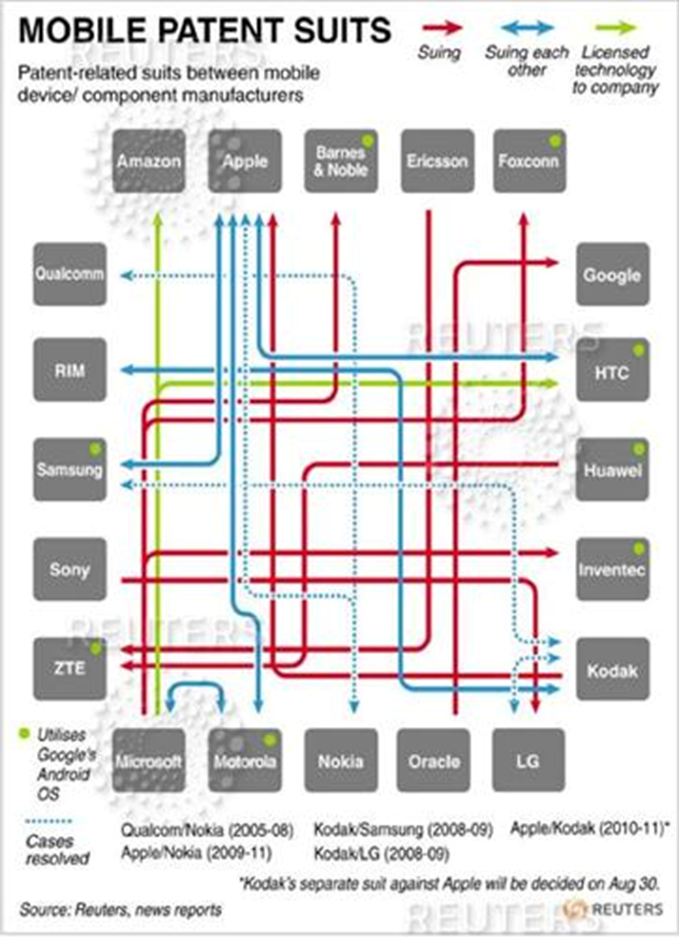
\includegraphics[width=0.7\linewidth]{Imagens/a8i1.png}
\end{figure}

\begin{figure}
    \centering
    \caption{A Guerra das patentes, segundo a “PCMag” (Jan. 2012)}
    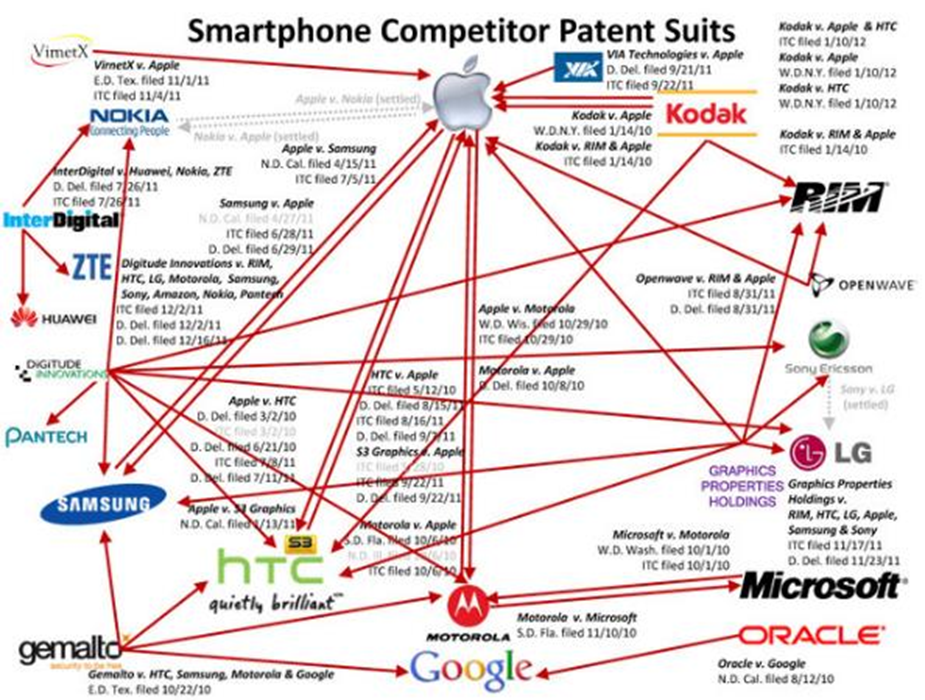
\includegraphics[width=0.7\linewidth]{Imagens/a8i2.png}
\end{figure}

\begin{figure}[H]
    \centering
    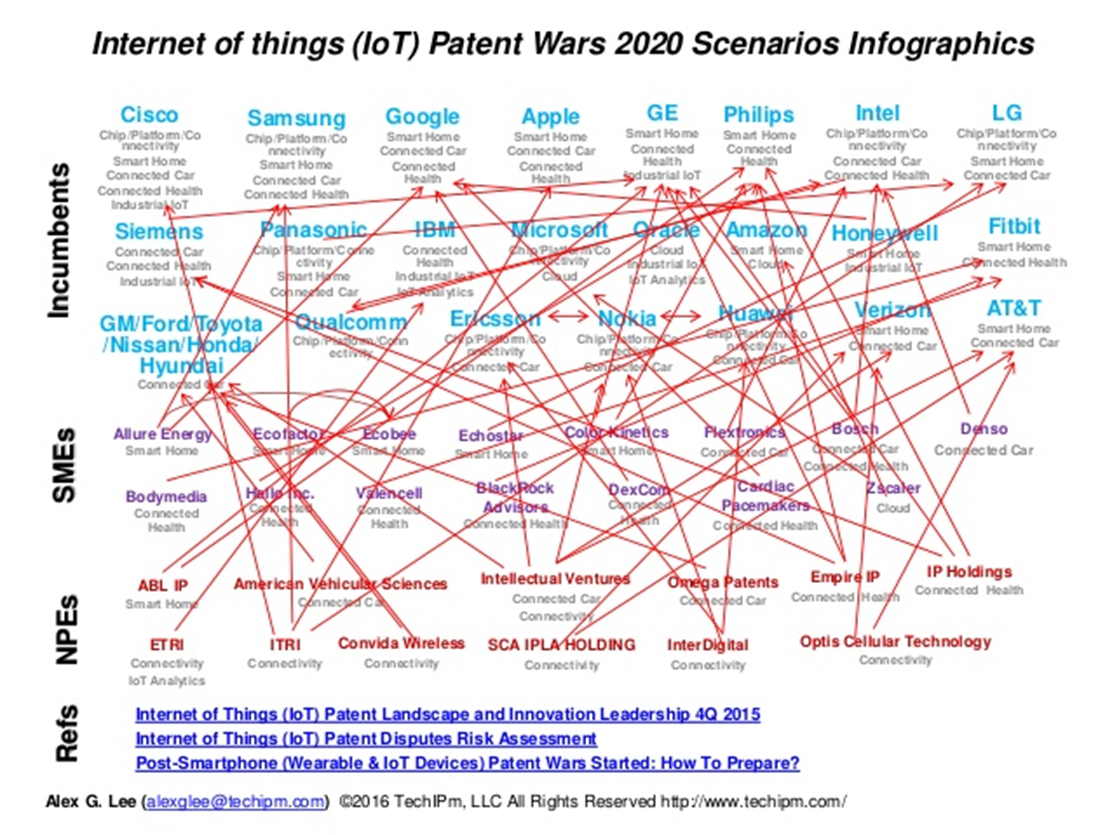
\includegraphics[width=0.7\linewidth]{Imagens/a8i3.png}
\end{figure}

\textbf{\textit{Uma estória paradigmática: o licenciamento compulsório dos medicamentos do coquetel anti HIV pelo governo brasileiro nos anos 2000…}}

\subsection{\textbf{Datas importantes do caso}}
\begin{enumerate}
    \item \textbf{1994}: Assinatura do TRIPS(Trade-Related Aspects of Intellectual Property Rights), da OMC (também pelo Brasil).
    \item \textbf{1996}: Lei da Propriedade Industrial (Lei 9.279).
    \item \textbf{1999}: Lei dos Genéricos (Lei 9.787).
    \item \textbf{2001}: \begin{itemize}
        \item início das negociações do governo brasileiro com as empresas farmacêuticas norte-americanas
        \item reclamação dos EUA na OMC
        \item lobby brasileiro junto à UNCHR
        \item primeiro licenciamento compulsório (Nelfinavir, da Roche)
    \end{itemize}
    \item \textbf{2007}: Licenciamento compulsório do Efavirenz (Merck).
\end{enumerate}

\subsection{\textbf{Condições possíveis para o licenciamento compulsório (Lei 9.279/96)}}
Detentor da patente abusa de seu poder econômico.

Detentor da patente não consegue produzir o produto patenteado no território brasileiro 3 anos após a concessão da patente.

As vendas locais não satisfazem as necessidades do mercado local.

Há dependência de uma patente sobre outra. 

Casos de emergência nacional ou interesse público.

\begin{figure}[H]
    \centering
    \caption{Tatiana S. NOGUEIRA, “Licenciamento compulsório e acesso ao tratamento do HIV/AIDS no Brasil” (2013)}
    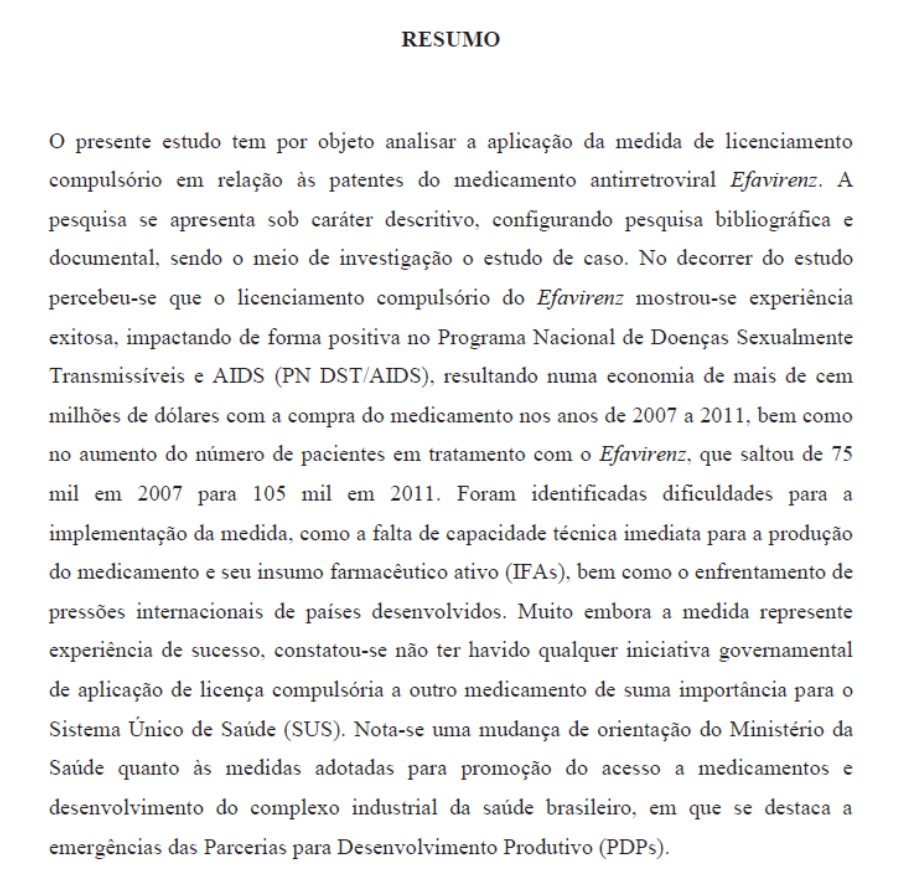
\includegraphics[width=0.7\linewidth]{Imagens/a8i4.png}
\end{figure}

\subsection{\textbf{Mais reflexões sobre o caso}}
Benoliel e Salama (2009)\begin{itemize}
    \item “É pouco provável que o Brasil estivesse melhor sem o licenciamento compulsório dos medicamentos do coquetel anti-AIDS.
    \item É duvidosa a hipótese de que leis de patentes mais rigorosas teriam tido efeitos significativos nos níveis de P\&D no Brasil.”
\end{itemize}

\subsection{\textbf{Discussões}}
Levando-se em consideração os materiais já discutidos na aula de hoje e os seguintes, discuta com os colegas:\begin{itemize}
    \item \href{https://archive.nytimes.com/opinionator.blogs.nytimes.com/2013/07/14/how-intellectual-property-reinforces-inequality/}{How Intellectual Property Reinforces Inequality,J.Stiglitz (2013)}
    \item \href{http://www.anpec.org.br/encontro2010/inscricao/arquivos/000-a3b50eba957afcc5a3f2a1895ca6485a.pdf}{Música e Pirataria na Universidade, Cortez e Madeira (2010).}
    \item \href{https://www.nature.com/articles/s41587-022-01485-x}{What the Covid-19 pandemic revealed about intellectual property”, R. Gold (2022).  }
    \item "Why Nations Fail?”, D. Acemoglu e J. Robinson, cap. 1, páginas 32 e 33
\end{itemize}

Que outras formas além de patentes poderiam ser adotadas para a proteção dos direitos de propriedade intelectual?

Como criar políticas e instituições que, de um lado, equilibram incentivos para a inovação com garantia de direitos de propriedade, e do outro, maximizam o bem-estar de toda a sociedade levando a resultados eficientes?

\newpage
\section{\textbf{Contratos}}
\subsection{\textbf{PACTA SUNT SERVANDA? O caso dos contratos de soja verde Christiane Leles Rezende e Decio Zylbersztajn (2007)}}

O desenvolvimento do complexo agroindustrial da soja no Brasil se deu [sic], em parte, como decorrência do surgimento de formas alternativas de crédito, tal como a venda antecipada de soja verde por meio de contratos. O problema que motivou este estudo foram as quebras contratuais por parte dos produtores rurais em um momento de expressiva alta do preço e suas consequentes disputas judiciais. Foram realizadas pesquisas quantitativas sobre 147 decisões judiciais do Tribunal de Justiça de Goiás e com 70 produtores rurais. Os testes realizados em decisões judiciais de primeira e segunda instância indicaram significante dispersão, apesar de tratarem-se do mesmo problema (…) no entanto a maior parte delas beneficiou os produtores rurais. 

\textit{Os efeitos das decisões já podem ser percebidos, como a maior exigência de garantias e a redução do número de contratos. Os produtores que não quebraram seus contratos também foram negativamente afetados com as novas estratégias adotadas pelas empresas compradoras de soja. O uso do conceito Função Social do Contrato gera um alto grau de instabilidade nos mesmos. Portanto, os custos de transação aumentaram para todos os agentes, bem como a importância de sanções econômicas.}

\begin{figure}[H]
    \centering
    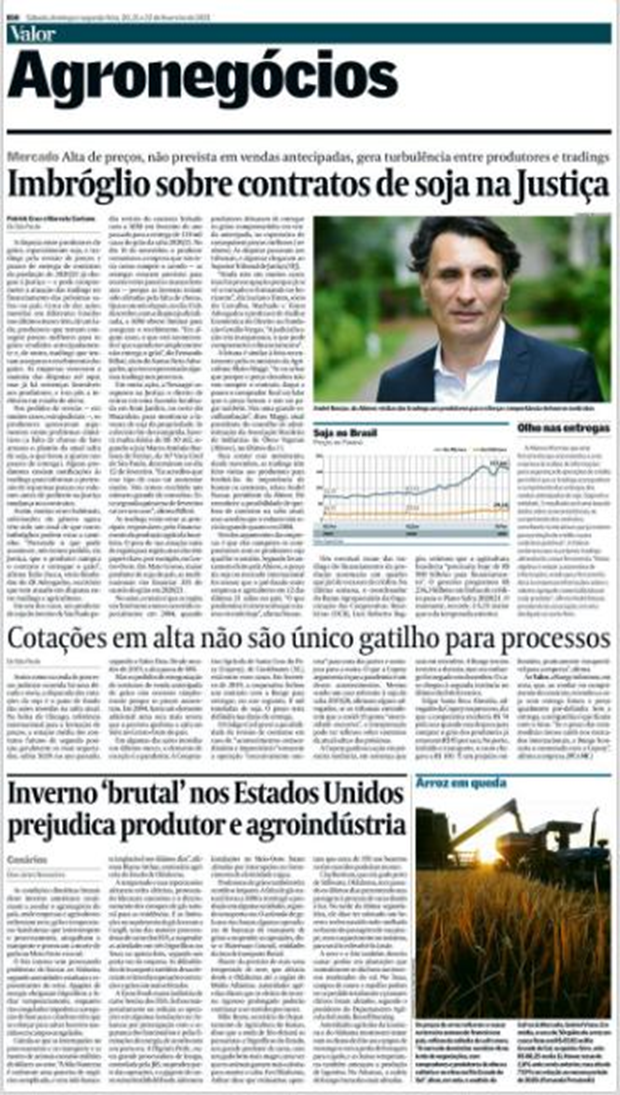
\includegraphics[width=0.4\linewidth]{Imagens/a10i1.png}
\end{figure}

\subsection{\textbf{O caso dos contratos de arrendamento mercantil (leasing)}}
Em meados da década de 90, era comum a aquisição de veículos através de contratos de arrendamento mercantil (leasing) atrelados ao dólar.

\begin{figure}[H]
    \centering
    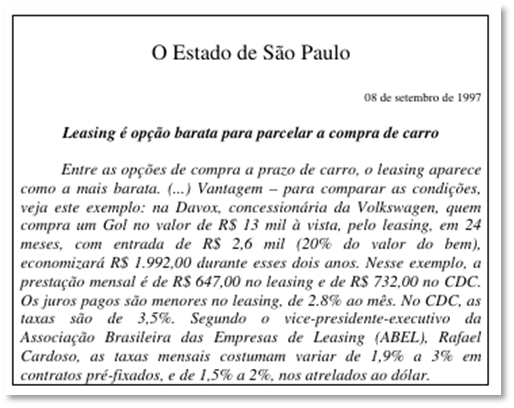
\includegraphics[width=0.5\linewidth]{Imagens/a10i2.png}
\end{figure}

\begin{figure}[H]
    \centering
    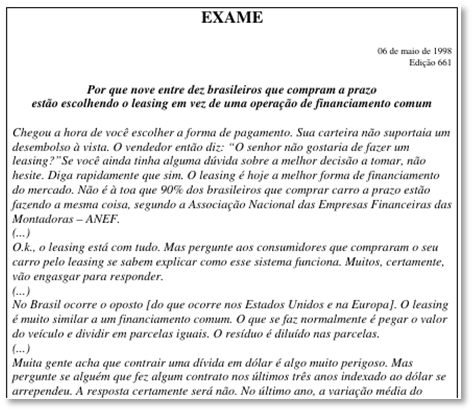
\includegraphics[width=0.5\linewidth]{Imagens/a10i3.png}
\end{figure}

Ocorre que, em janeiro de 1999 houve uma brutal desvalorização cambial, levando à judicialização.

\begin{figure}[H]
    \centering
    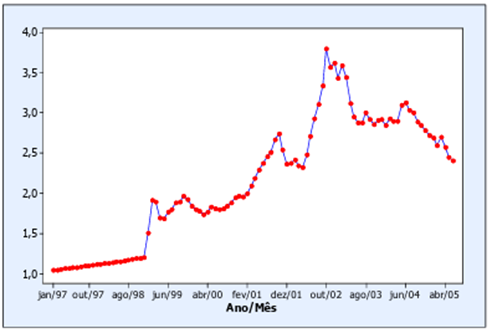
\includegraphics[width=0.5\linewidth]{Imagens/a10i4.png}
\end{figure}

\begin{figure}[H]
    \centering
    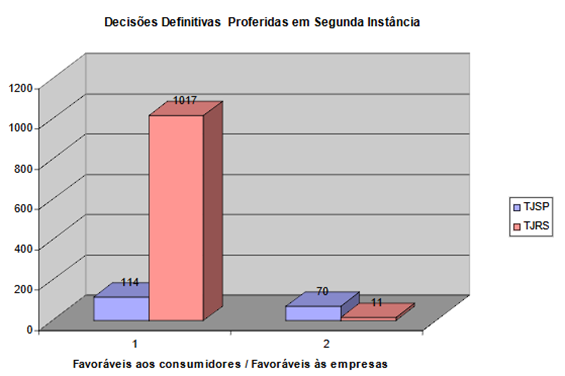
\includegraphics[width=0.5\linewidth]{Imagens/a10i5.png}
\end{figure}

\begin{figure}[H]
    \centering
    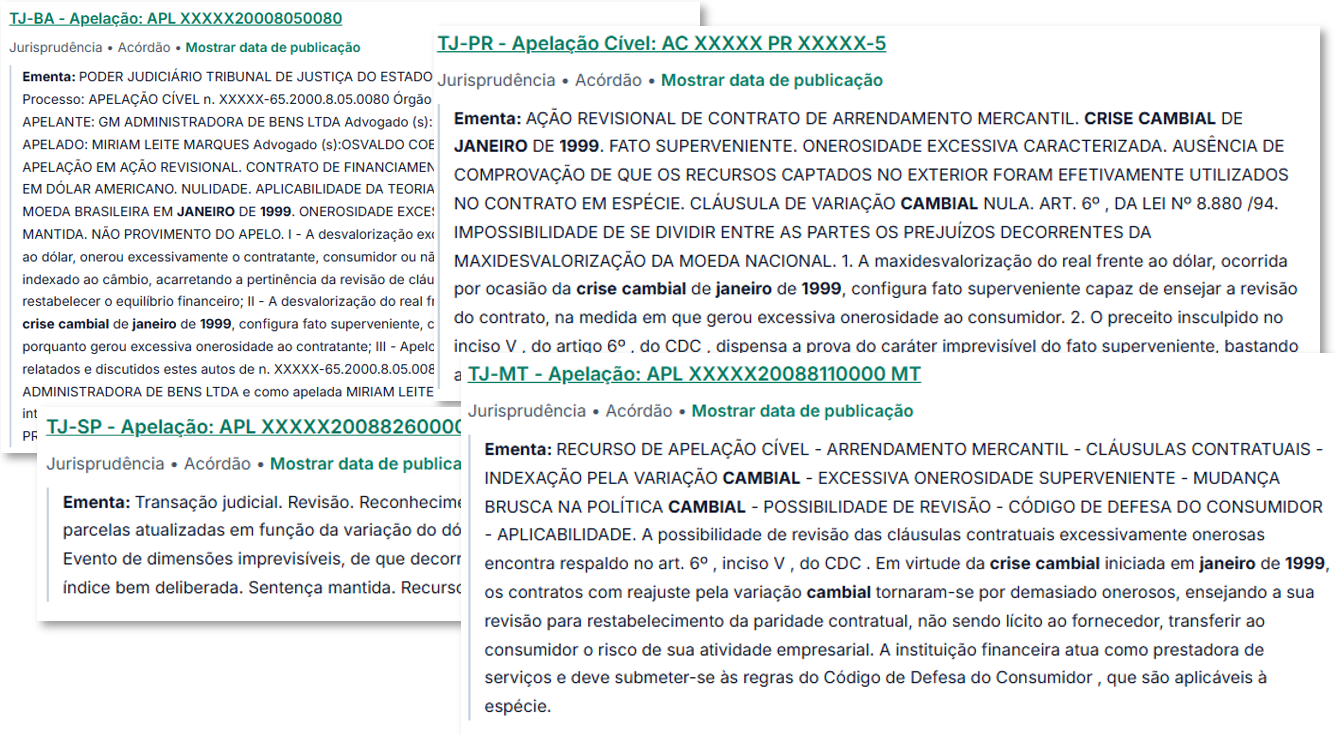
\includegraphics[width=0.7\linewidth]{Imagens/a10i6.png}
\end{figure}

\subsection{\textbf{Mais um caso: quebra de contratos na COVID... }}
E-mail recebido por mim, no dia 08 abril de 2020, de um juiz do TJ-SP:

"Estamos recebendo uma avalanche de pedidos de revisionais de aluguel em razão da pandemia, sob o fundamento da força maior e impossibilidade de cumprimento do contrato. Pensei em deferir as tutelas em 50\% do valor, mas aí ponderei com o risco da atividade e que talvez só diluiria o prejuízo, quebrando credor e devedor. Muito pior. Do ponto de vista econômico, o que pensa ser o mais indicado ?”

\subsection{\textbf{Contratos e Crescimento Econômico}}
“\textit{The inability of societies to develop effective, low-cost enforcement of contracts is the most important source of both historical stagnation and contemporary underdevelopment in the third world}”. \textbf{Douglass North (1990)}

\subsection{\textbf{O que é um contrato?}}

O que é um contrato?\begin{itemize}
    \item Que tipos de promessas podem ser considerados contratos?
    \begin{itemize}
        \item Contratos informais é contrato?
    \end{itemize}
\end{itemize}

O que é um “bom” direito contratual?\begin{itemize}
    \item “Bom” para quem?
    \begin{itemize}
        \item Partes x sociedade
    \end{itemize}
\end{itemize}

Existe alguma justificativa para proteger o não-cumprimento de promessas?

\textbf{\textit{Dissonância Cognitiva}}: frustração recíproca de expectativas (diferente da má fé), comunicação equivocada com confusão daquilo que era esperado tanto do vendedor como do comprador. 

Má Fé, propaganda enganosa, engano doloso. 
Promessas unilaterais, plano futuro, “notória mudança de estado”, “Onerosidade excessiva”, etc.

Estas justificativas jurídicas para não reconhecimento, ou não cumprimento da promessa, fazem sentido econômico?

Quais das situações são contratos abaixo? O que define? \begin{enumerate}
    \item Uma pessoa promete vender a outra um Notebook por R\$ 500. O negócio é feito e, quando chega em casa, o comprador descobre que o Notebook está em péssimo estado: o teclado não funciona direito e a tela está trincada. Furiosa, ela exige seu dinheiro de volta e quer devolver o Notebook. O vendedor se espanta: o comprador achava mesmo que, por R\$ 500, estava adquirindo um Notebook em estado de novo?
    \begin{itemize}
        \item Dissonância Cognitiva: frustração recíproca de expectativas (diferente da má fé), comunicação equivocada com confusão daquilo que era esperado tanto do vendedor como do comprador. \(\rightarrow\) O contrato pode ser desfeito com consentimento de ambas as partes.
    \end{itemize}

    \item Uma senhora adquire pelo correio um método de emagrecimento por R\$1.000. Quando chega a encomenda, ela descobre que o “método” nada mais era do que um rolo de esparadrapo com as seguintes instruções: “Feche a boca!”
    \begin{itemize}
        \item Propaganda Enganosa! \(\rightarrow\) Código de Defesa do Consumidor Brasileiro. 
    \end{itemize}

    \item Um pai promete à filha uma maravilhosa festa de 15 anos. No entanto, ele entra em falência e não consegue cumprir a promessa. A mãe da menina, sua ex-mulher, resolve processá-lo.
    \begin{itemize}
        \item Promessa = Contrato?
        \begin{itemize}
	        \item Promessas unilaterais;
	        \item Plano futuro;
	        \item “Notória mudança de estado”;
	        \item “Onerosidade excessiva”;
	        \item etc.
        \end{itemize}
    \end{itemize} 
\end{enumerate}


\subsection{\textbf{Análise Econômica dos Contratos}}
Análise econômica dos contratos pressupõe:\begin{itemize}
    \item \textbf{cooperação} mútua entre os agentes.
    \item \textbf{disposição voluntária} dos agentes (para distribuição dos ganhos ou perdas em uma transferência de direitos de propriedade).
\end{itemize}

\textbf{Coase}: “Trocas são transferências de direitos de propriedade”. 

\textbf{Contrato}: representa uma transferência mútua de direitos entre as partes.

Contratos (para os economistas) permitem:\begin{itemize}
    \item Realizar trocas;
    \item Transferir riscos;
    \item Resolver problemas de eficiência alocativa.
\end{itemize}

\subsection{\textbf{Teoria dos Contratos Eficientes}}

\textbf{Contratos completos} são perfeitos e eficientes:\begin{itemize}
    \item Todos os estados da natureza são previstos.
    \item Todos os riscos são alocados para quem pode arcá-los com menor custo.
    \item Toda informação relevante foi comunicada.
    \item Todos os ganhos de cooperação possíveis entre as partes foram obtidos.
\end{itemize}


Agentes racionais desenham contratos completos na ausência de custos de transação.

Quando um contrato não menciona um risco, então ele tem uma \textbf{lacuna}, ou seja, é \textbf{incompleto}(todos os contratos são incompletos, dado que ninguém consegue prever o futuro).

Deve-se sempre \textbf{obrigar} o cumprimento dos contratos? 

Às vezes, isso pode ser dogmático e não-responsivo (ineficiente).

O que é resolver uma disputa contratual de forma dogmática? E de forma responsiva?\begin{itemize}
    \item Uma decisão dogmática sacrifica a maximização de eficiência/bem-estar apenas com o objetivo de cumprir a regra legal/contratual.
    \item Uma decisão responsiva, por sua vez, preocupa-se, em primeiro lugar, com a maximização de eficiência/bem-estar.
\end{itemize}

“Quebras contratuais eficientes” no sentido de Kaldor- Hicks. \begin{itemize}
    \item Pode ser mais eficiente permitir que uma das partes rompa o contrato e indenize a outra parte do que obrigar o cumprimento do contrato.
\end{itemize}

\subsection{\textbf{Escusas à execução: Regulamentação dos Contratos}}
Se estas hipóteses não forem observadas, a anulação do contrato pela lei (regulamentação) é eficiente!

\begin{figure}[H]
    \centering
    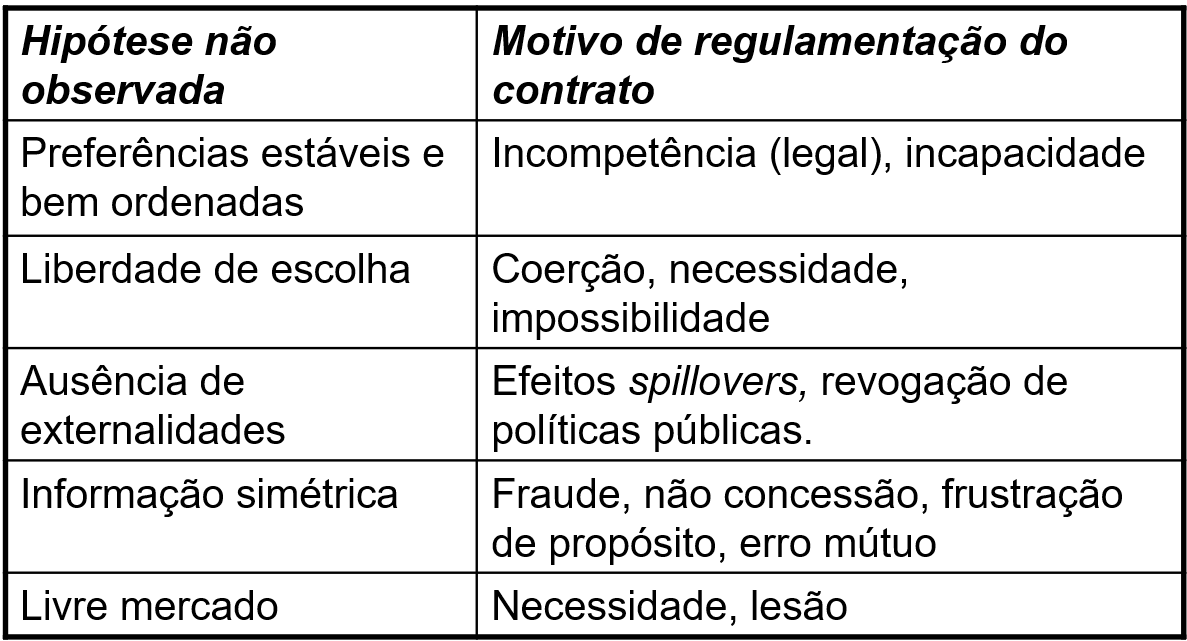
\includegraphics[width=0.7\linewidth]{Imagens/a10i7.png}
\end{figure}

\subsection{\textbf{"Default Rules" para preenchimento de lacunas contratuais}}
Custos de transação e limitação cognitiva fazem com que os contratos sejam inerentemente incompletos.\begin{itemize} 
    \item Por exemplo: discutir cláusulas financeiras ou traição no contrato matrimonial.
\end{itemize}

Contratos incompletos têm lacunas deixadas propositadamente ou não. 

Para quê estudar contratos completos então?\begin{itemize}
    \item Para que sirvam como parâmetro do que seguir – tal como aconteceu com o exercício mental feita por Coase para resolver problemas de alocação de direitos de propriedade.  
\end{itemize}

\subsubsection{\textbf{“Default Rules” e barganhas hipotéticas: Problema}}
Uma empresa construtora fecha um contrato com uma família para a construção de uma casa. Materiais a serem usados e seus respectivos preços são fechados. Durante a construção há um aumento substancial de um dos materiais, que acaba elevando muito o preço final da obra. 

A família se nega a pagar este aumento e a empresa processa o cliente para conseguir o pagamento. Como o juiz(a) deve decidir este conflito?

\textbf{Situação 1}:\begin{itemize}
    \item A construtora sabe que o preço do mármore Carrara pode subir em \$5000 devido ao aumento da demanda pelo produto com probabilidade de 0.4.
    \item O custo adicional esperado é de \( 5000 \times 0.4 = \$2000 \).
    \item A construtora pode se precaver deste risco fazendo um hedge por \$500, o que produz uma economia de \$1500.
    \item O cliente não pode prever o aumento súbito no preço do mármore pois desconhece as características do mercado de mármore.
    \item A construtora falha em se precaver do risco e apresenta uma conta de \$5000 extra ao contratante, que se recusa a pagar.
    \item A empresa construtora é: Tomadora de Risco Eficiente (\textit{“Cheapest cost avoider”}) \(\Rightarrow 100\%\).
\end{itemize}

\textbf{Situação 2}:\begin{itemize}
    \item Agora, suponha que a causa do aumento no preço do mármore não pudesse ter sido prevista por nenhuma das partes, por exemplo, que o aumento decorresse de um terremoto no local da jazida.
    \item \textbf{O que fazer?}
    \item A empresa continua sendo \textbf{Tomadora de Risco Eficiente (TRE)}, porém parcial.
\end{itemize}

\subsubsection{\textbf{“Default Rules” e barganhas hipotéticas}}
Como a justiça deve preencher as falhas de um contrato?\begin{itemize}
    \item A lei pode (deve) induzir comportamento eficiente reduzindo custos de transação [Teorema de Coase normativo].
    \item Decisões judiciais criam regras (padrões) para falha nos contratos.
    \item Termos padrões (default rules) eficientes permitem menos custos de transação nas alocações de riscos nos contratos.
\end{itemize}

Quem deve ser o responsável em assumir riscos num contrato?\(\rightarrow\)\textbf{Tomador de risco eficiente} (efficient risk-bearer ; TRE): a parte que tem o menor custo em lidar com o risco.

Regra eficiente: Deve-se resolver a quebra do contrato com a solução que as partes teriam concordado caso elas tivessem negociado sem custos de transação (\textbf{barganha hipotética}).\begin{itemize} 
    \item Teorema de Coase Normativo
\end{itemize}

Barganha hipotética: contrato ideal ex-post, sem que ela tenha efetivamente acontecido ex-ante. \begin{itemize}
    \item Identifica o tomador de risco mais eficiente.
\end{itemize}

É como se houvesse um contrato com custo de transação zero.

\textbf{Situação 1:} Dado que o construtor poderia, ou mesmo, deveria ter previsto o aumento de preço mais facilmente do que o contratante, ele deveria ter negociado um contrato que o compensasse por assumir o risco. (Ele é o tomador de risco mais eficiente).

\textbf{Situação 2}:\begin{itemize}
    \item Nesta situação, o juiz continuaria atribuindo a responsabilidade à construtora, porém ele poderia revisar o preço do contrato.
    \item O contrato ideal alocaria o risco à construtora  por, por exemplo, \$4.500. 
    \item Então, o cliente arcaria com um custo extra de \$500 pelo serviço de prevenção de risco (hedge), e o restante, \$4.500, seria a perda da construtora por não ter arcado com o risco da perda de \$ 5.000.
\end{itemize}

\subsection{\textbf{Outra fonte de incompletude de contratos: assimetrias de informação}}
\begin{itemize}
    \item Agente-Principal (ou Problema de Agência)
    \item Seleção Adversa
    \item Risco moral (moral \textit{hazard})
\end{itemize}

Soluções:\begin{itemize}
    \item Sinalização 
    \item Screening
    \item Desenho de contratos mais completos. 
\end{itemize}

\textbf{Questões}\begin{enumerate}
    \item Qual é definição de cada um dos problemas de assimetria de informação acima mencionados?
    \item Quais seriam exemplos de cada um dos casos?
    \item Há formas de resolvê-los via desenho de contratos?
\end{enumerate}

\subsection{\textbf{Problema do Agente-Principal (ou Problema de Agência)}}
O problema do agente principal ocorre quando os \textbf{agentes}(pelo menos um) têm metas diferentes das metas de seus \textbf{principais}(pelo menos um), ou seja, seus problemas de maximização diferem do problema de maximização dos seus agentes.

O principal que induzir uma outra pessoa, o agente, a tomar alguma ação. 

O principal não observa a ação do agente, mas somente o resultado da ação, um produto x .\(\rightarrow\)\textbf{\textit{Hidden-Action}}

Problema para o principal: pagar \(s(x)\) ao agente para induzi-lo a tomar a ação desejada.

Há duas (ou mais) ações possíveis pelo agente: a ou b (não observáveis pelo principal), gerando \(x(a)\) e \(x(b)\) (observáveis), mas custam \(c(a)\) e \(c(b)\) aos agentes.

Utilidade do principal:\( x – s(x)\)

Utilidade do agente: \(s(x) – c(a)\) ou \(c(b)\)

Problema ao principal: criar \(s(\cdot)\) que maximize sua utilidade, sujeito às restrições impostas pelo comportamento otimizador do agente (oportunidades fora, ou escolher b ao invés de a, ou vice-versa). 

\textbf{Exemplo real:} empregador e empregado; agente e seu mandante; cliente e advogado, etc.

\subsection{\textbf{Risco Moral (Moral Hazard)}}
A parte segurada têm ações que não podem ser observadas (\textit{hidden actions}) pela seguradora, mas que podem afetar a probabilidade de um sinistro ocorrer ou a magnitude de seu pagamento(mudanças de comportamento).

\textbf{Exemplos}:\begin{itemize}
    \item Seguro contra acidentes e comportamento “desleixado”.
    \item \href{https://money.cnn.com/galleries/2009/news/0909/gallery.highest_paid_worst_CEOs/index.html}{CEO e acionistas.}Aqui temos\begin{itemize}
        \item Um Problema de Agente (suas prioridades são diferentes de quem o contratou)
        \item Um problema de \textit{Moral Hazard}
    \end{itemize}
\end{itemize}

\subsection{\textbf{Problema do Seleção Adversa}}
Por causa de assimetria de informações em mercados onde existem produtos de diferente qualidade, somente um preço pode ser cobrado no equilíbrio; dessa forma, produtos de baixa qualidade “expulsam” os produtos de alta qualidade. 

\textbf{Exemplos:}\begin{itemize}
    \item Mercado dos limões: carros usados ruins e bons. 
    \item Seguro de saúde e pessoas mais doentes.
    \item Mercado de crédito, spread de juros e proteção ao hipossuficiente pelo judiciário brasileiro.
\end{itemize}

\subsection{\textbf{Prof. George Akerloff – Prêmio Nobel de Economia 2001, pelo estudo do processo de sinalização}}
\begin{figure}[H]
    \centering
    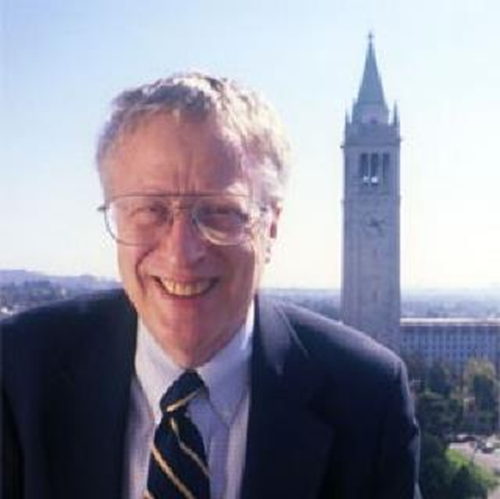
\includegraphics[width=0.7\linewidth]{Imagens/a11i1.png}
\end{figure}

Estudou o famoso caso do mercado de “\textbf{\textit{limões}}”.

\subsection{\textbf{Sinalização x Screening}}
Como resolver as assimetrias de informação?\begin{itemize}
    \item Sinalização (\textit{signalling}) e \textit{Screening}.
\end{itemize}

\textbf{Sinalização}: maneira pela qual \textbf{vendedores enviam sinais aos compradores}, transmitindo informações sobre a qualidade do produto que, não fosse assim, não poderiam ser observadas.

\subsection{\textbf{Prof. Michael Spence – Prêmio Nobel de Economia 2001, pelo estudo do processo de sinalização}}

\begin{figure}
    \centering
    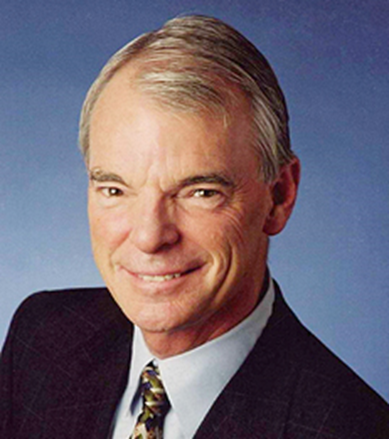
\includegraphics[width=0.5\linewidth]{Imagens/a11i2.png}
\end{figure}

Formulou o modelo de sinalização no mercado de trabalho.

\subsection{\textbf{Sinalização}}
\textbf{Hipóteses}:\begin{itemize}
    \item Há dois tipos de trabalhadores: alta produtividade e baixa produtividade e não há como diferenciá-los diretamente;
    \item Salário oferecido será um valor ponderado de suas produtividades marginais, onde a ponderação é a probabilidade de encontrar um tipo de trabalhador e outro;
    \item Trabalhador de alta produtividade ganhará menos do que sua real produtividade \(\rightarrow\) querem sinalizar que são de alta produtividade;
    \item Sinal deve ser tão forte tal que os trabalhadores de baixa produtividade não consigam adquiri-lo, ou conseguem somente a um custo muito mais alto: restrições de auto-seleção (\textit{self selection});
    \item Com este sinal, haverá equilíbrio separador.
    \item Outros exemplos de sinalização?
\end{itemize}

\subsection{\textbf{Screening}}
No screening, a parte que tem menos informação tentar coletar a informação separando os tipos de qualidades diferentes.\begin{itemize}
    \item \textbf{Exemplos}: processos de trainee, busca de informações sobre qualidade dos produtos, etc. 
\end{itemize}


Equilíbrio agregador (\textit{\textbf{pooling equilibrium}}): Os dois tipos de trabalhadores aceitam o mesmo tipo de contrato.

Equilíbrio separador (\textit{\textbf{separating equilibrium}}): Diferentes tipos de trabalhadores aceitam diferentes tipos de contratos.

Hipóteses:\begin{itemize}
    \item Múltiplas firmas empregadoras: lucro econômico zero;
    \item Dois tipos de trabalhadores: de alta qualidade e de baixa qualidade;
    \item Hidden information;
    \item Todas as firmas oferecem o mesmo conjunto de contratos;
    \item Custo zero para o processo de screening.
\end{itemize}

Equilíbrios possíveis:\begin{itemize}
    \item A firma representativa oferece um único tipo de contrato (salário) que atrai os dois tipos de trabalhadores.
    \item A firma representativa oferece um único tipo de contrato (salário) que atrai somente um tipo de trabalhador.
    \item A firma representativa oferece dois tipos de contratos (salários), um para cada tipo de trabalhador.
\end{itemize}

\subsection{\textbf{Relembrando os casos passados}}
Em cada um dos casos, havia assimetria de informação, para além de informações imperfeitas? Se sim, a favor de quem, em prejuízo de quem?

A resolução eficiente da quebra de contrato muda algo, levando-se em conta a resposta anterior?

Como explicar a resolução dos casos seguintes?

\subsection{\textbf{Como podemos explicar pela AED?}}
\begin{enumerate}
    \item Sou inquilino de um terreno com algumas construções. Antes do fim do contrato, algumas destas construções pegam fogo. O common law afirma que devo pagar todo o restante dos meses de aluguel até o fim do contrato, pois o risco de incêndio deve ser arcado por conta do inquilino e não do proprietário.
    \item Faço a venda de um terreno e aceito como pagamento moedas de ouro. Dois anos depois, descubro que as moedas são falsas, e tento cancelar a venda. Porém, fico sabendo que meu comprador já fez a revenda e fugiu da cidade. Entro com processo para reaver meu terreno, alegando que o atual proprietário nunca de fato se apropriou dele, pois a primeira venda foi baseada numa fraude. Eu perco a ação. O juiz diz que eu poderia ter recuperado o terreno caso o meu comprador ainda fosse o “proprietário”, mas este terceiro indivíduo é inocente. 
    \item Ao invés de comprar meu terreno com moedas falsas, o indivíduo falsifica a escritura e vende para um terceiro. Quando eu processo este comprador inocente, eu ganho o caso e reavejo meu terreno. 
\end{enumerate}

\textbf{O que justifica estas decisões?}

\subsection{\textbf{Calculando Danos}}
Vamos analisar um caso famoso de contratos do direito norte-americano: \href{https://www.youtube.com/watch?v=_983pIQ_0sw}{Hawkins vs McGee}

Como podemos calcular remédios e indenizações/danos nesse caso de quebra contratual?

Existem três formas igualmente possíveis, e igualmente econômicas:\begin{itemize}
    \item Danos de expectativas (frustradas).
    \item Danos de confiança (frustradas) .
    \item Danos de custos de oportunidades (perdidas), ou danos de restituição.
\end{itemize}

\subsubsection{\textbf{Danos de Expectativas}}
Esses danos de quebra contratual compensam o beneficiário da promessa pelo dano causado com o não-cumprimento da promessa pelo promitente. 

Os\textbf{ danos de expectativas} serão calculados baseados no valor do cumprimento do contrato, que\textbf{\textit{ deixaria a vítima de quebra contratual na posição em que ela estaria se o promitente tivesse cumprido a promessa.}}

\subsubsection{\textbf{Danos de Confiança}}
A quebra contratual deixa o beneficiário da promessa em uma situação pior do que se não tivesse feito contrato algum. 

Os \textbf{danos de confiança} serão calculados baseados no valor de “inexistência do contrato”, que \textbf{\textit{deixaria a vítima de quebra contratual numa posição em que estaria se ela nunca tivesse contratado com o promitente.}}

\subsubsection{\textbf{Danos de Custos de Oportunidades}}
Engajar-se em um contrato normalmente envolve a perda da oportunidade de ter um contrato alternativo. 

Os \textbf{danos de custos de oportunidade} serão calculados baseados no valor da oportunidade perdida, que \textit{\textbf{deixaria a vítima da quebra contratual na posição em que ela estaria se ela tivesse assinado o contrato que era a melhor alternativa àquele que foi quebrado.}} \begin{itemize}
    \item Em outras palavras, esse dano substitui o valor da oportunidade perdida.
\end{itemize}

\subsection{\textbf{Exercício Aplicado}}
Como podemos calcular remédios e danos nesse caso de quebra contratual?\begin{enumerate}
   \item Danos de expectativas.
   \item Danos de confiança.
   \item Danos de custos de oportunidades.
\end{enumerate}

Assuma que a mão do pequeno Hawkins  estava em uma condição ruim; assuma que o Dr. McGee prometeu uma mão perfeita com a cirurgia. Contudo, o que ocorreu foi que, após a intervenção cirúrgica, a mão de Hawkins ficou pior do que estava antes. Assuma, finalmente, que na cidade, havia um outro médico, Dr. McDonald, que poderia ter melhorado a situação da mão de Hawkins, mas não tê-la deixado em condição perfeita. 

Mostre o que cada um dos danos envolveria em termos de valores. As 3 regras concederão o mesmo valor? Se não, qual concederá a maior indenização? Qual a menor?

\begin{figure}[H]
    \centering
    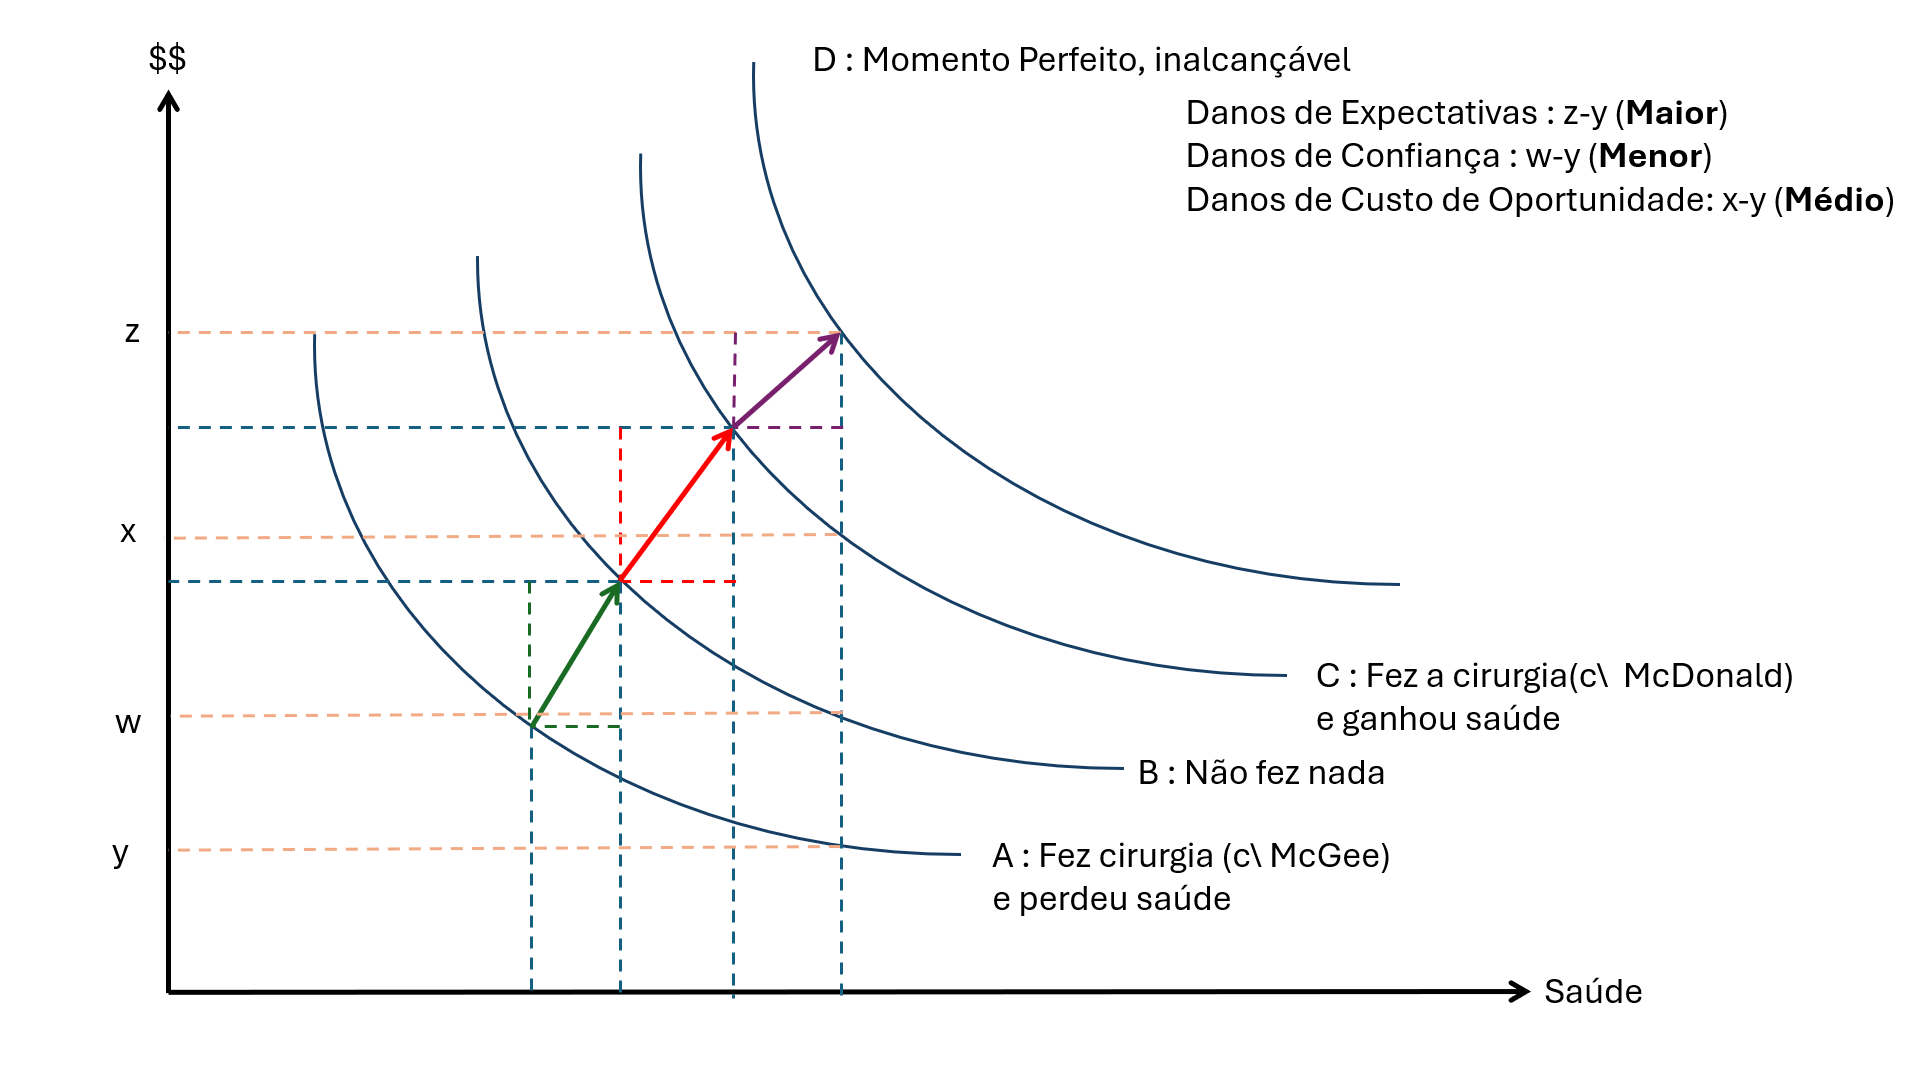
\includegraphics[width=0.7\linewidth]{Imagens/a12i4.png}
\end{figure}

\subsection{\textbf{Calculando Danos}}
Vamos usar o modelo microeconômico!

Qual foi o valor final?\begin{itemize}
    \item Na 1ª instância, Hawkins ganhou \$1.400 dólares de indenização. 
    \item Depois da apelação de McGee, foi concedido \$800 dólares** mais honorários advocatícios. 
\end{itemize}

Nos valores de hoje (2025):\begin{itemize}
    \item US\$ 26.123,67
    \item US\$\$ 14.927,81
\end{itemize}

\subsection{\textbf{Análise Econômica do Processo Judicial (Civil)}}
\subsubsection{\textbf{Um modelo econômico do processo judicial}}
Fazer parte de um processo judicial envolve várias decisões e várias etapas (por isso, um “processo”), com probabilidades diferentes de ganho ou perda de um valor \$X.

Como será a decisão de uma Pessoa ao longo do processo?

Primeiro, vamos entender a estrutura básica do Judiciário brasileiro.

\subsubsection{\textbf{De maneira sintética…}}
\begin{figure}[H]
    \centering
    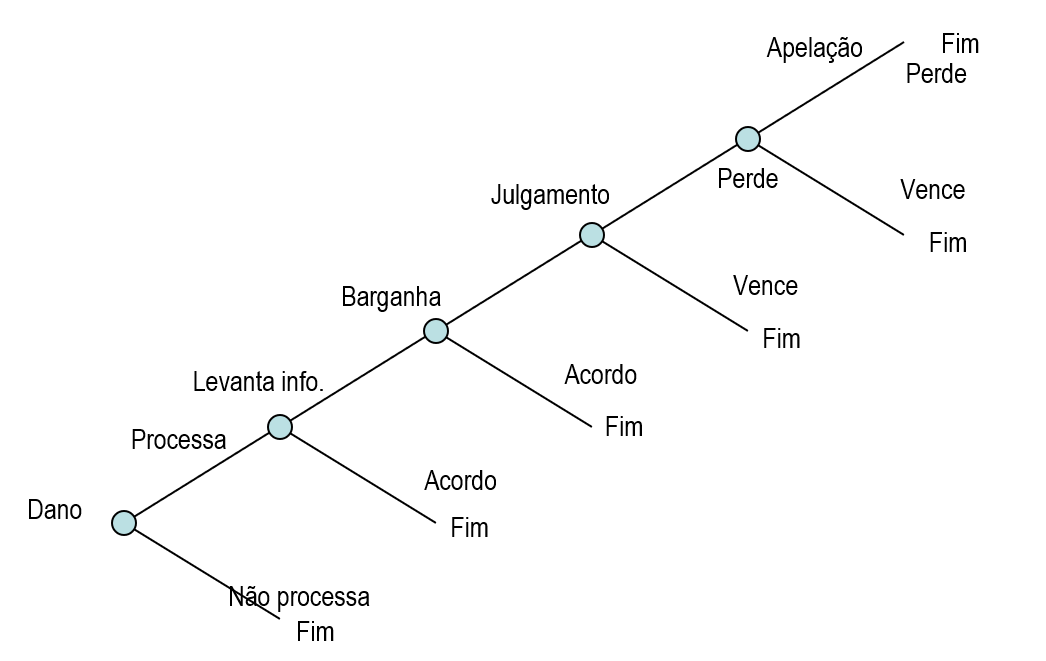
\includegraphics[width=0.7\linewidth]{Imagens/a12i1.png}
\end{figure}

\subsubsection{\textbf{Vale a pena processar?}}
\begin{figure}[H]
    \centering
    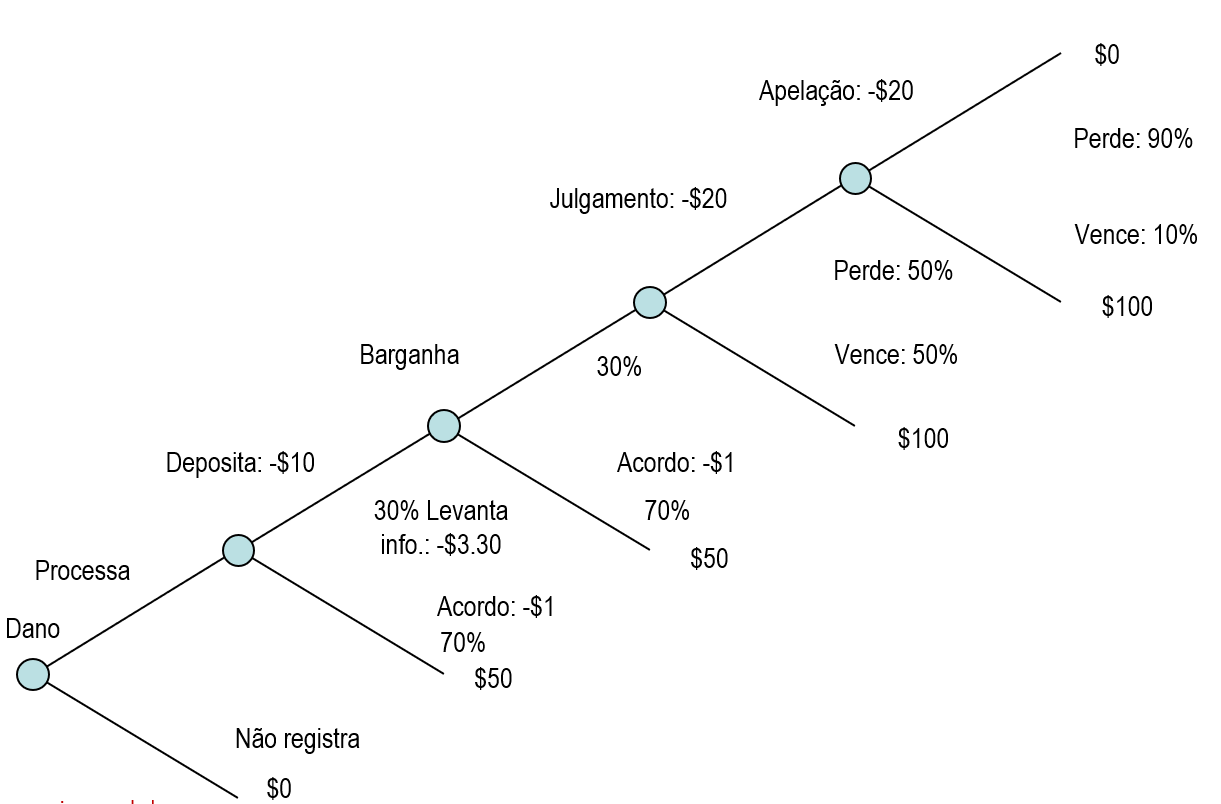
\includegraphics[width=0.7\linewidth]{Imagens/a12i2.png}
\end{figure}

\textbf{Como saber se o indivíduo economicamente  racional decidirá por processar ou não?}

\begin{figure}[H]
    \centering
    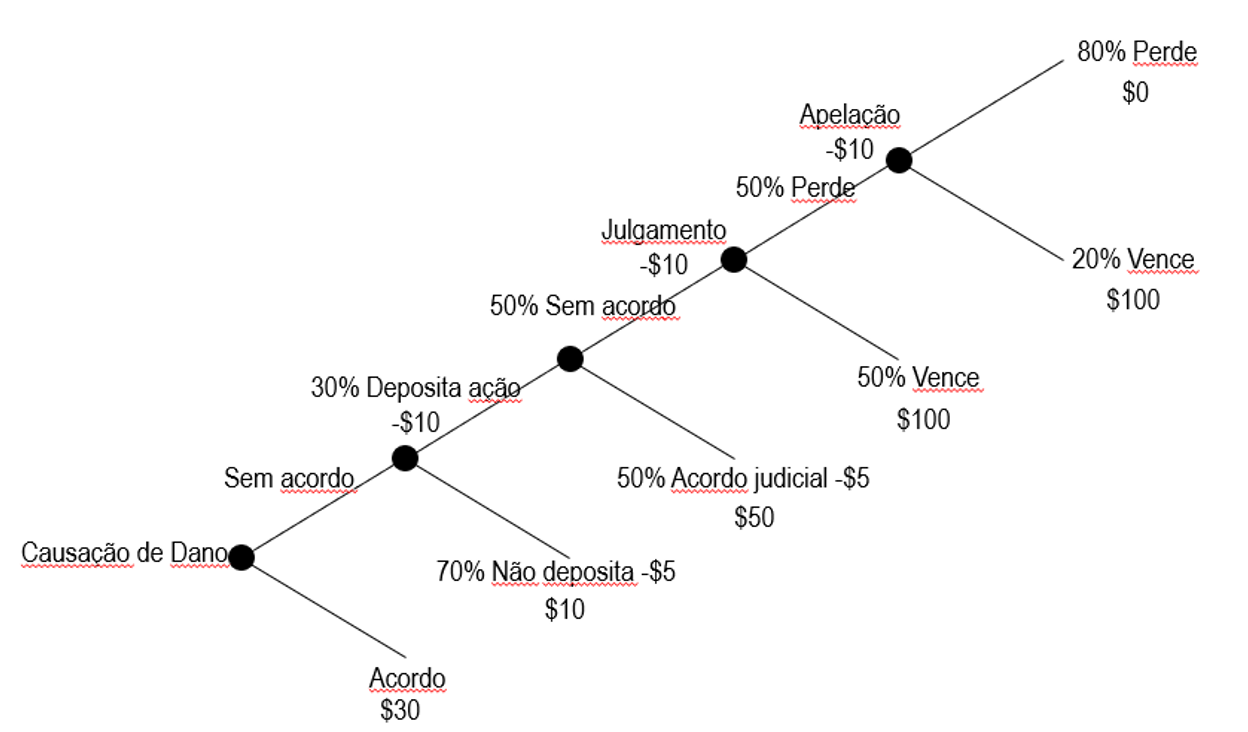
\includegraphics[width=0.7\linewidth]{Imagens/a12i3.png}
\end{figure}

\textbf{Como saber se o indivíduo economicamente  racional decidirá por processar ou não?}

\newpage
\section{\textbf{Análise Econômica do Processo Judicial (Civil) e do Judiciário}}
\subsection{\textbf{Estrutura do Judiciário brasileiro}}
\begin{figure}[H]
    \centering
    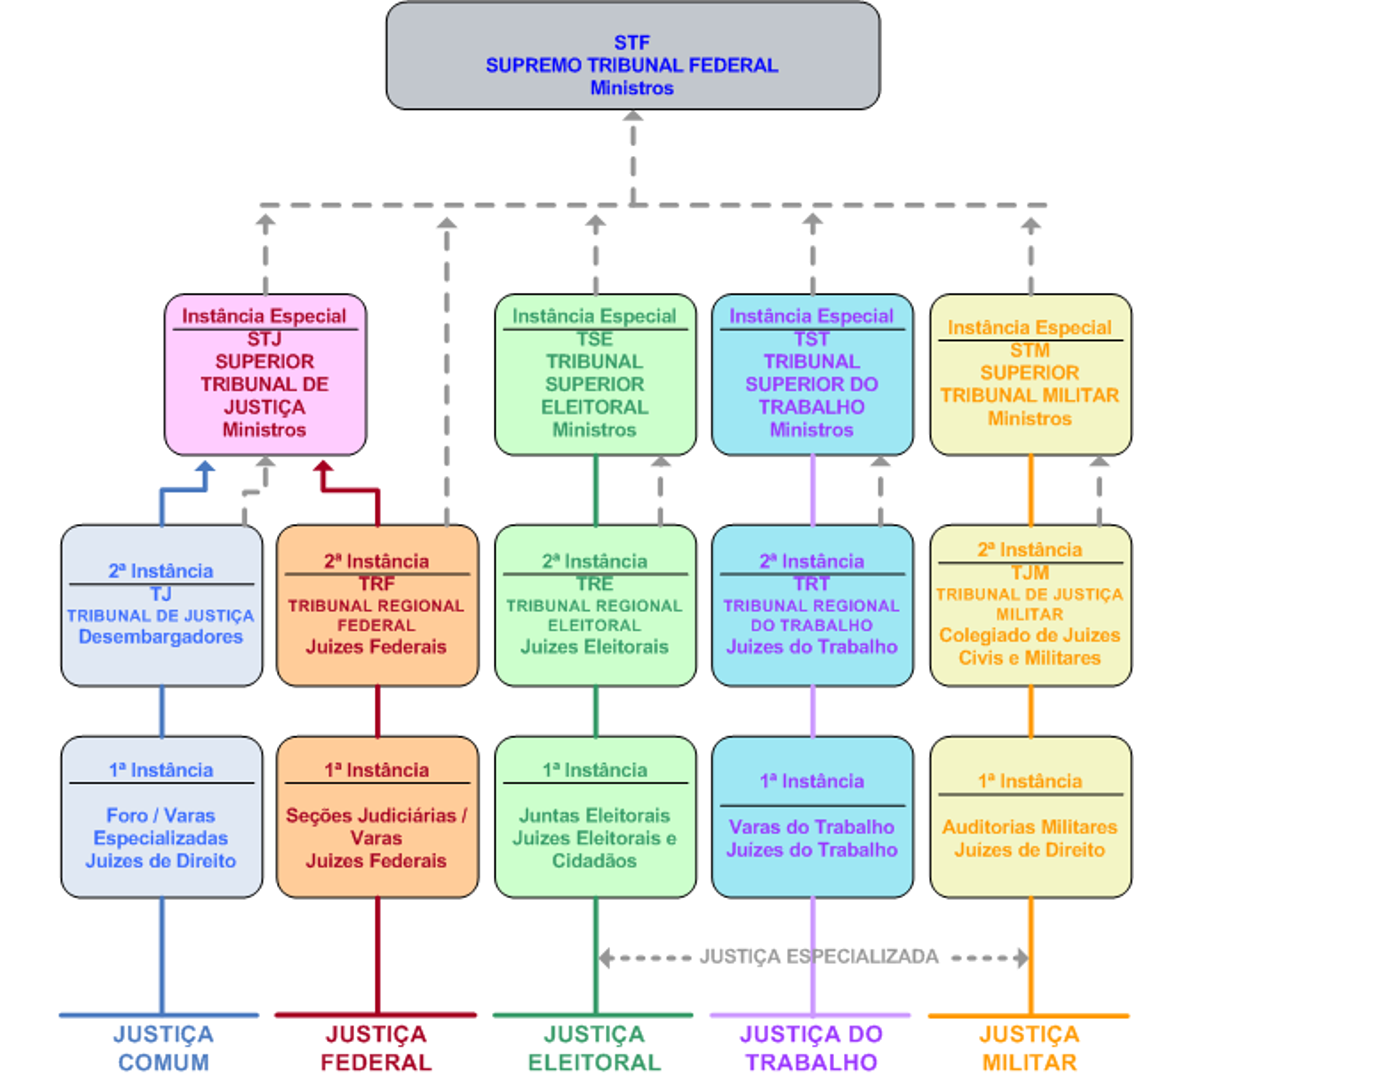
\includegraphics[width=0.7\linewidth]{Imagens/a13i1.png}
\end{figure}



\subsection{\textbf{Um modelo econômico do processo judicial}}
Fazer parte de um processo judicial envolve várias decisões e várias etapas (por isso, um “processo”), com probabilidades diferentes de ganho ou perda de um valor \$X.

Como será a decisão de uma Pessoa ao longo do processo?

Primeiro, vamos entender a estrutura básica do Judiciário brasileiro.

\subsubsection{\textbf{De maneira sintética}}
\begin{figure}[H]
    \centering
    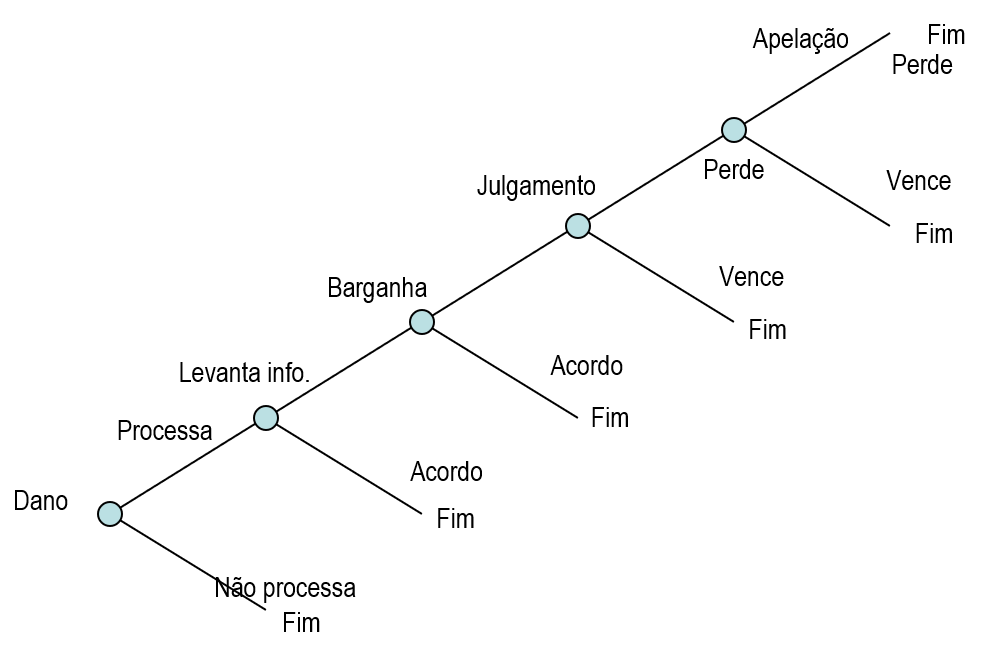
\includegraphics[width=0.7\linewidth]{Imagens/a13i2.png}
\end{figure}

\subsubsection{\textbf{Vale a pena processar?}}
\begin{figure}[H]
    \centering
    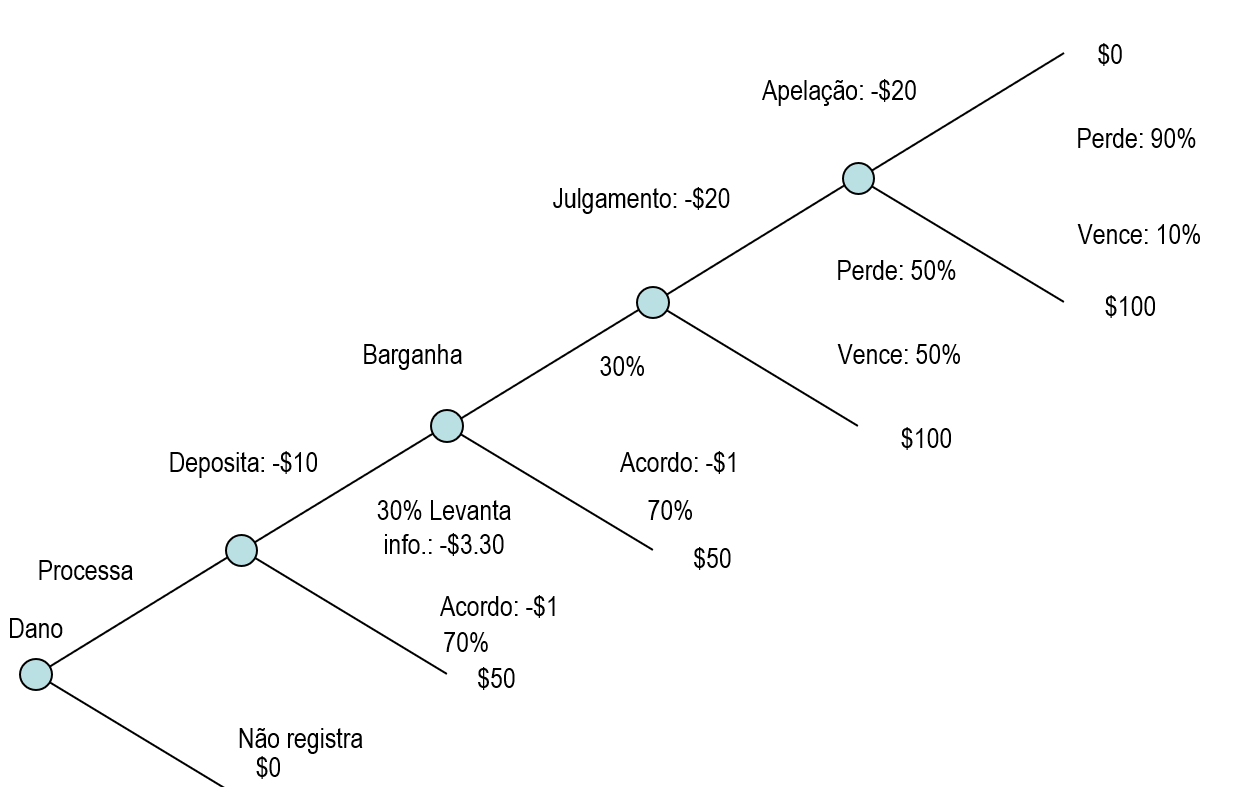
\includegraphics[width=0.7\linewidth]{Imagens/a13i3.png}
\end{figure}

\textbf{Como saber se o indivíduo economicamente  racional decidirá por processar ou não?}

\begin{figure}[H]
    \centering
    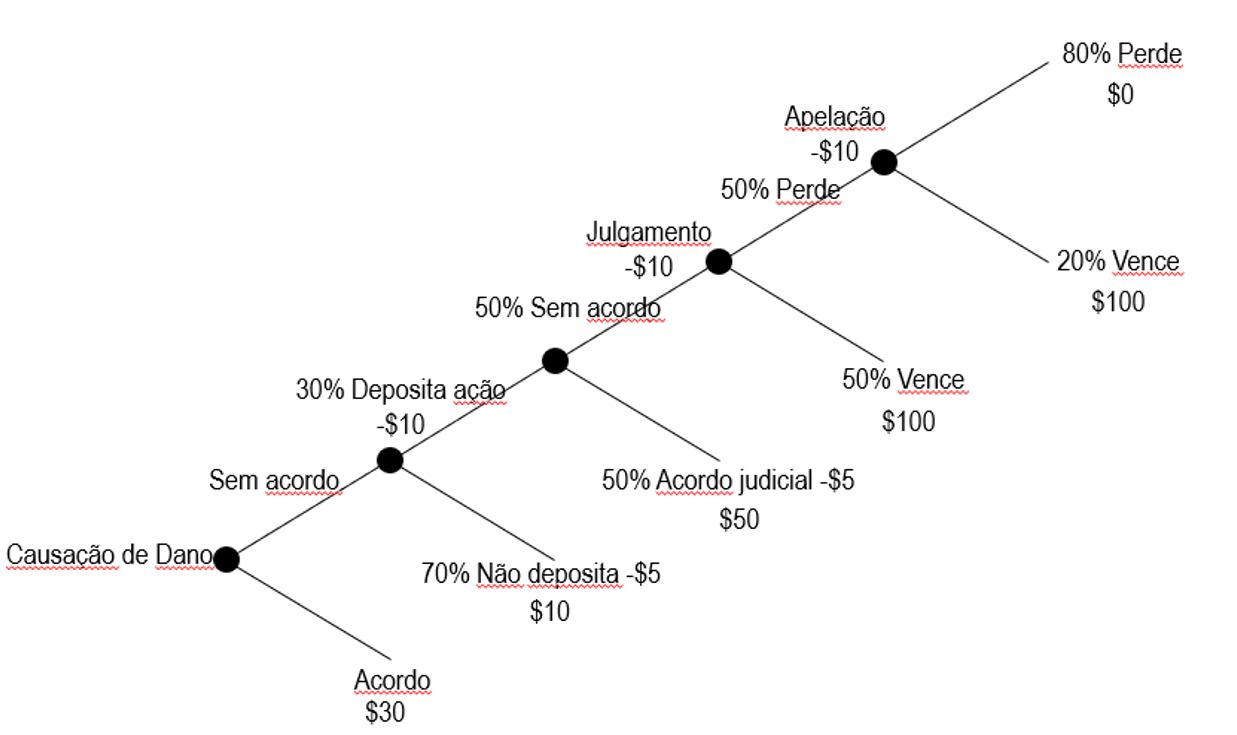
\includegraphics[width=0.5\linewidth]{Imagens/a13i4.png}
\end{figure}

\textbf{Como saber se o indivíduo economicamente  racional decidirá por processar ou não?}
Vamos fazer o valor esperado desse jogo, mas por meio de uma indução retroativa.
Vale a pena fazer acordo

\subsection{\textbf{Comportamento Judicial}}
Como que os juízes decidem?\begin{itemize}
    \item Positivo x Normativo
\end{itemize}

Acepção jurídica: juiz como intérprete da norma\begin{itemize}
    \item Aplicação objetiva das normas aos fatos dos casos
    \item Regras de interpretação jurídica (hermenêutica)
    \item Pouco espaço para variação (discricionariedade)
\end{itemize}

Mas a realidade não é bem assim...\begin{itemize}
    \item Decisões são muito frequentemente reformadas por instâncias superiores: mais de 50\% (Yeung, 2010)
    \item Tribunais mudam de opinião (ex. prisão em segunda instância...)
    \item Advogados tentam escolher juízes que vão julgar seus casos (ex. HCs no STF)
\end{itemize}

\subsection{\textbf{Motivação}}
Além disso...\begin{itemize}
    \item Políticos se importam muito com indicação de juízes para tribunais
    \item Se juiz é interprete imparcial da norma, como explicamos esses fatos?
\end{itemize}

Exemplos:\begin{itemize}
    \item Robert Bork (1987) - \url{https://www.youtube.com/watch?v=Xza0MfDXZlE} 
 (min 2:00)
    \item Elena Kagan (2010) - \url{https://www.youtube.com/watch?v=XFkVwvlpXUk } (opening statement)
    \item Elena Kagan (2010) - \url{https://www.youtube.com/watch?v=ooAtySpObLw } (piada)
    \item André Mendonça (2021)  - \url{https://www.youtube.com/watch?v=p2cOYdRIpKo}
\end{itemize}

\begin{figure}[H]
    \centering
    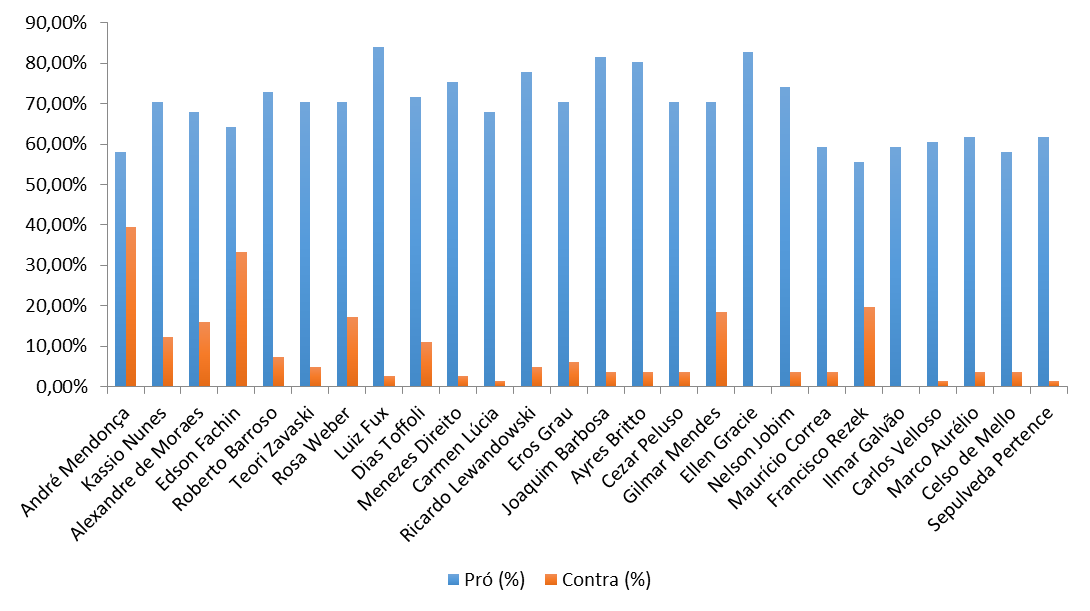
\includegraphics[width=0.7\linewidth]{Imagens/a13i5.png}
\end{figure}

“Muito criticado por advogados e juristas, ‘realismo jurídico’ nada mais é do que o reconhecimento de que os juízes não decidem as disputas através da aplicação objetiva da lei aos fatos do caso. \textbf{Que, na realidade, as crenças e preconcepções dos juízes, que são correlacionadas com suas características individuais como raça, gênero, religião, background socioeconômico e, mormente, afiliação política, têm impactos sobre as decisões que emitem na atividade de julgador”.  }

\textbf{Assim, explicações estritamente jurídicas do comportamento dos juízes é claramente insuficiente.}

\textbf{Precisamos recorrer à economia, ciência política, psicologia, sociologia, etc.}

\subsection{\textbf{O desenvolvimento do campo}}
\begin{figure}[H]
    \centering
    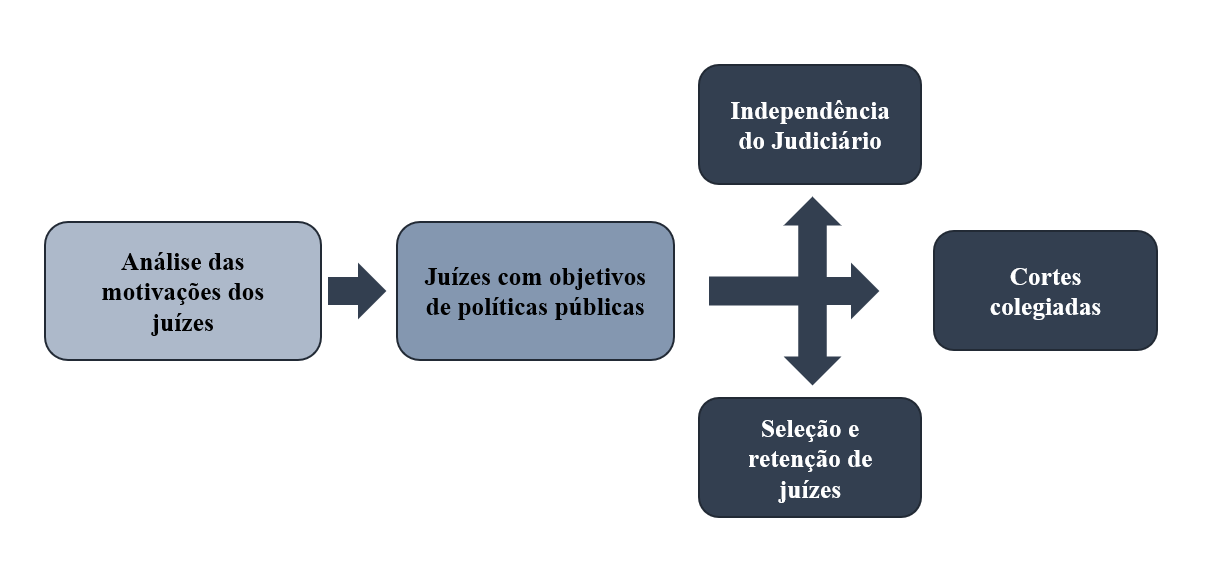
\includegraphics[width=0.7\linewidth]{Imagens/a13i6.png}
\end{figure}

\begin{figure}[H]
    \centering
    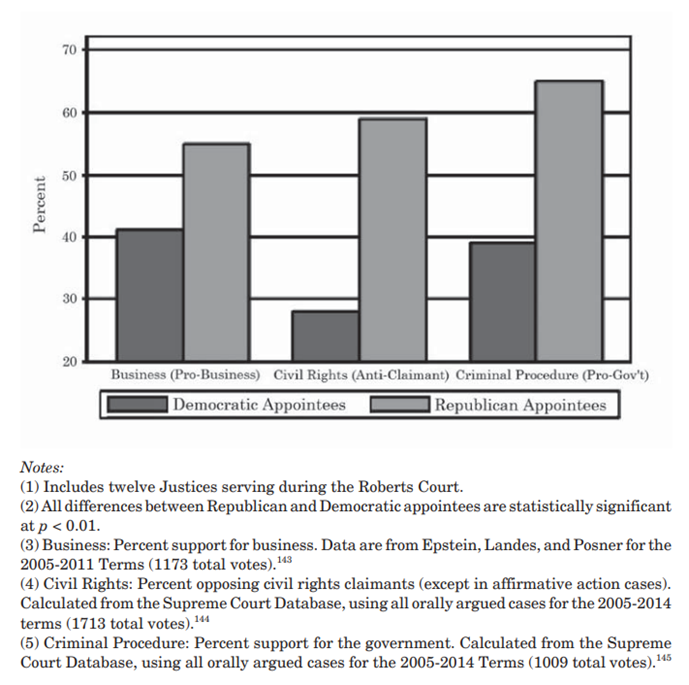
\includegraphics[width=0.7\linewidth]{Imagens/a13i7.png}
\end{figure}

\begin{figure}[H]
    \centering
    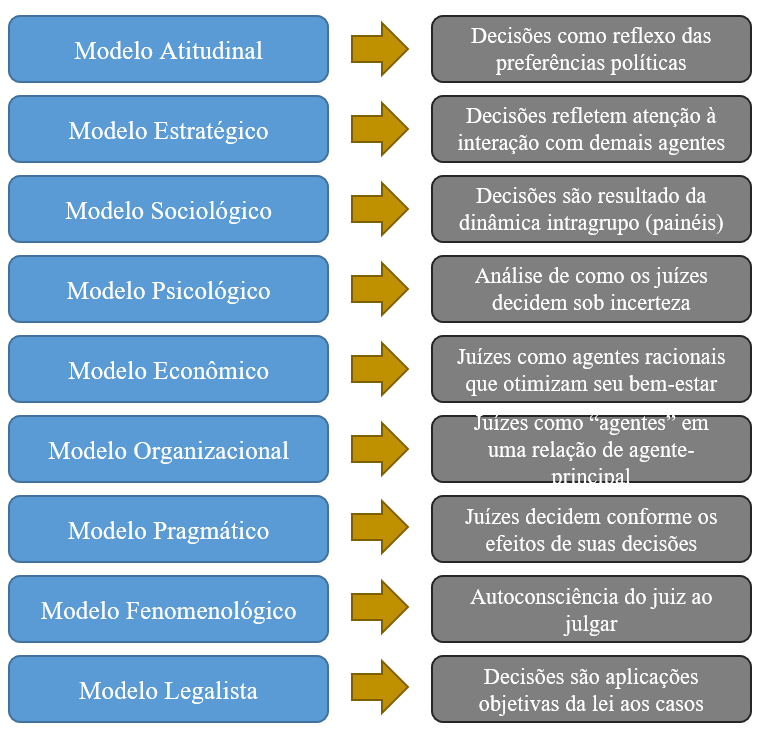
\includegraphics[width=0.7\linewidth]{Imagens/a13i8.png}
\end{figure}

\begin{figure}[H]
    \centering
    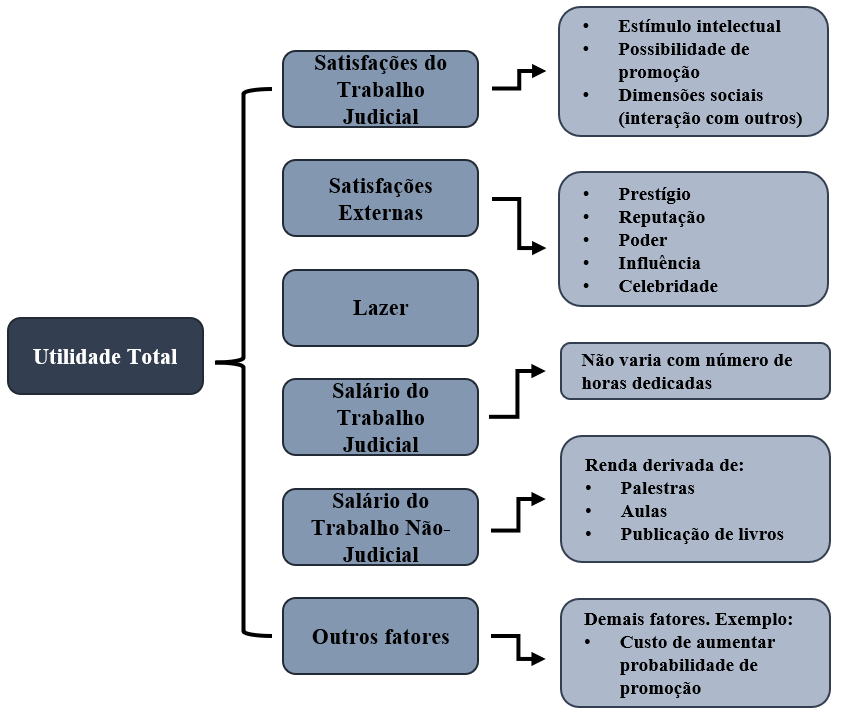
\includegraphics[width=0.7\linewidth]{Imagens/a13i9.png}
\end{figure}

\newpage
\section{\textbf{Estado, Provisão de Bens Públicos}}
\subsection{\textbf{Da nossa 2a aula do semestre…}}
Relaxando a hipótese do mercado competitivo… \begin{itemize}
    \item Competição imperfeita
    \item Externalidades
    \item Bens Públicos
    \item Informação Imperfeita e Assimétrica
    \item Distribuição
    \item Custos de transação entre outros
   \item  enfim, Falhas de Mercado.
\end{itemize}

É por isso tudo que, em situações normais, mercados não serão capazes de alcançar a eficiência de maneira livre, cooperativa. O Estado será necessário!

\subsection{\textbf{E Mais...}}
Crescimento x Distribuição

 Objetivos de curto prazo x longo prazo
 
 Estabilidade interna x externa

Necessidade de coordenação de decisões, dados os conflitos gerados pelo enfoque das políticas (como acima).

\subsection{\textbf{O caso dos bens públicos}}

\textbf{Bens Públicos} : Bens que seu consumo é não excludente(proibir o consumo da pessoa mediante ao pagamento) e não rival(o consumo feito por uma pessoa não impede(dada a redução) na quantidade ofertada).

\subsubsection{\textbf{Provisão de Bens Públicos}}

\begin{table}[H]
\centering
\begin{tabular}{|cl|cc|}
\hline
\multicolumn{2}{|c|}{\multirow{2}{*}{\textbf{}}}                            & \multicolumn{2}{c|}{\textit{\textbf{Tem Consumo Rival ?}}}                                                                            \\ \cline{3-4} 
\multicolumn{2}{|c|}{}                                                      & \multicolumn{1}{c|}{Sim}       & Não                                                                                                  \\ \hline
\multicolumn{1}{|r|}{\multirow{2}{*}{\textit{\textbf{É excludente}}}} & Sim & \multicolumn{1}{c|}{Bem Rival} &                                                                                                      \\ \cline{2-4} 
\multicolumn{1}{|r|}{}                                                & Não & \multicolumn{1}{c|}{}          & \begin{tabular}[c]{@{}c@{}}Bem Público Puro\\ (segurança pública,\\ iluminação de vias)\end{tabular} \\ \hline
\end{tabular}
\end{table}

\begin{table}[H]
\centering
\begin{tabular}{|cl|cc|}
\hline
\multicolumn{2}{|c|}{\multirow{2}{*}{\textbf{}}}                            & \multicolumn{2}{c|}{\textit{\textbf{Tem Consumo Rival ?}}}                                                                                                                                                                \\ \cline{3-4} 
\multicolumn{2}{|c|}{}                                                      & \multicolumn{1}{c|}{Sim}                                                                                           & Não                                                                                                  \\ \hline
\multicolumn{1}{|r|}{\multirow{2}{*}{\textit{\textbf{É excludente}}}} & Sim & \multicolumn{1}{c|}{Bem Rival}                                                                                     & \begin{tabular}[c]{@{}c@{}}Bem Público Impuro\\ (TC a cabo, informação)\end{tabular}                 \\ \cline{2-4} 
\multicolumn{1}{|r|}{}                                                & \begin{tabular}[c]{@{}l@{}}Não\\ Não "vendável"\end{tabular}  & \multicolumn{1}{c|}{\begin{tabular}[c]{@{}c@{}}Bem público impuro\\ (calçada lotada,\\ praia lotada)\end{tabular}} & \begin{tabular}[c]{@{}c@{}}Bem Público Puro\\ (segurança pública,\\ iluminação de vias)\\ Carona(\textit{Free Rider};Trajédia dos Comuns)\\ Exaustão(vira bem Rival)\end{tabular} \\ \hline
\end{tabular}
\end{table}



\subsubsection{\textbf{Soluções}}
Criação de direitos de propriedade quando bens públicos puros passam a ser impuros, ou bens privados. 

Quando mantiverem natureza de bens públicos, somente o Estado pode resolver – pois não seria lucrativo para agentes privados ofertarem…

Mas…  

\subsubsection{\textbf{Mas…}}
O caso dos faróis de Coase…

\begin{figure}[H]
    \centering
    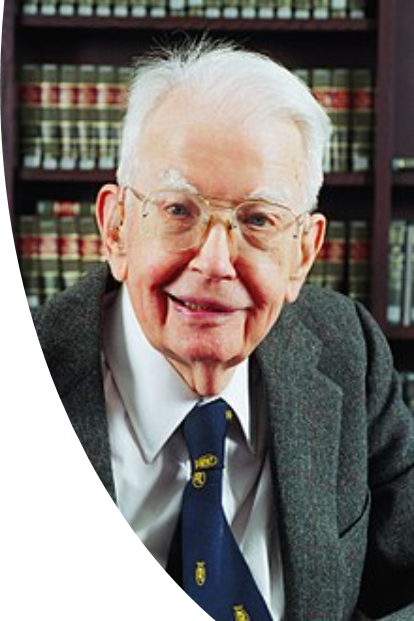
\includegraphics[width=0.5\linewidth]{Imagens/a14i1.png}
\end{figure}

Em um famoso paper de 1974, Coase argumentou que, mesmo sendo típicos bens públicos, os faróis britânicos eram providos por empresas privadas  até 1842 (ver interessante discussão na página 192 de Gruber).

“No entanto, em  um famoso artigo de 1974, Ronald Coase (do Teorema de Coase) conduziu uma pesquisa histórica mostrando que os faróis Britânicos haviam sido ofertados de maneira bem-sucedida por empresas privadas muito antes de o governo apossar-se da tarefa. Indivíduos privados, sentindo oportunidades de lucro, obtiveram permissões do governo para construir faróis e cobrar pedágios nos portos onde os navios ancoravam. Esses indivíduos determinavam quantos faróis cada navio passou em sua rota e daí cobravam o pedágio de acordo. Então, os faróis foram ofertados de maneira bem-sucedida pelo mercado privado até o ano de 1842, a partir do qual, o governo Britânico comprou todos os faróis privados para ofertar publicamente este bem em particular”.

\textit{*Segundo Coase (1974), a razão oferecida pelo governo para a aquisição dos faróis e a oferta pública do serviço era que isso levaria à preços mais baixos, prevenindo os proprietários privados dos faróis de inflacionarem os preços do pedágio. Coase então mostra que, depois da estatização dos faróis, não foi observada a redução nos preços dos pedágios...}

\subsubsection{\textbf{Provisão privada de bem-público: Quando ocorre?}}
\href{https://g1.globo.com/jornal-nacional/noticia/2024/01/20/moradores-se-unem-para-reconstruir-ponte-que-foi-destruida-por-enchente-no-rio-grande-do-sul.ghtml}{Alguns valorizam mais o bem público do que outro, ou estão mais dispostos a pagar do que outros.}

Altruísmo: custos e benefícios de terceiros entram na decisão do consumo de determinado indivíduo.\begin{itemize}
    \item Capital social: confiança e oferta privada de bens públicos são positivamente correlacionados.OCDE Society at a Glance 2016
\end{itemize}

“Warm glow model”: derivação de satisfação privada ao fazer bem ou ofertar bens públicos para os outros. \begin{itemize}
    \item Explicações de comportamentos tradicionalmente descritos como desvios de racionalidade.     
    \item Nenhuma consegue resolver integralmente a escassez da oferta privada de bens públicos.
\end{itemize}

\subsubsection{\textbf{Educação: bem público ou privado?}}
Educação, ou melhor, escolas, são bem \textbf{privado}, pois têm consumo rival e excludente. 

Por que então governos oferecem educação?

Grandes Externalidades:\begin{itemize}
    \item Cidadania (“capital humano bem público”: Mancur Olson, 1996);
    \item Falhas no mercado de crédito;
    \item Miopia no consumo das famílias;
    \item Redistribuição de renda (por ex.: inércia educacional no Brasil).
\end{itemize}

\subsubsection{\textbf{“Conclusão”}}
Bens públicos são oferecidos de maneira mais eficiente pelo Estado. Mas, lembrar faróis de Coase (1974).

Bens privados são oferecidos de maneira mais eficiente pelo mercado privado. Mas, há os casos de bens privados com externalidades.

\subsection{\textbf{Como oferecer bens públicos?}}
\subsubsection{\textbf{Votação majoritária e provisão de bem público}}
A provisão de bem público é frequentemente determinada pelo \textbf{processo político}, via votação, seja via \textbf{democracia direta ou democracia representativa.}

Decisões via \textbf{votação majoritária} geram provisão eficiente do bem público?

\subsubsection{\textbf{Art. 1º da Constituição Federal/1988}}
“A República Federativa do Brasil, formada pela união indissolúvel dos Estados e Municípios e do Distrito Federal, constitui-se em Estado Democrático de Direito e tem como fundamentos:

I – a soberania;

II – a cidadania;

III – a dignidade da pessoa humana;

IV – os valores sociais do trabalho e da livre iniciativa; 

V – o pluralismo político.

\textbf{Parágrafo único. Todo poder emana do povo, que o exerce por meio de representantes eleitos ou diretamente, nos termos desta Constituição”. }

\subsubsection{\textbf{Mecanismos de votações diretas }}

Ou seja, no geral, a democracia no Brasil (e em quase todos os países do mundo) dá se de maneira \textbf{indireta, via representantes eleitos. }

Exceções:\begin{itemize}
    \item Plebiscitos
    \item Referendos
    \item Iniciativas populares (mas sem garantia de se tornarem normas legais): art.5º, LXXXIII.
\end{itemize}

\subsubsection{\textbf{Ações Populares que viraram leis}}
\href{https://oglobo.globo.com/brasil/comissao-aprova-nova-tramitacao-para-projetos-de-iniciativa-popular-21285077}{Link}\begin{enumerate}
    \item Lei 8.930/ 1994 (Daniella Perez): incluiu o homicídio qualificado na Lei de Crimes Hediondos (8.072, de 1990).
    \item Lei 9.840/1999: combate à compra de votos.
    \item Lei 11.124/2005: Fundo Nacional de Habitação de Interesse Social.
    \item Lei Complementar 135/2010: a Lei da Ficha Limpa.
\end{enumerate}

\subsubsection{\textbf{Votação majoritária (direta)}}
Na votação majoritária, ou por maioria, a opção que recebe a maioria dos votos é implementada.

Começando com um exemplo de sociedade com 3 grupos diferentes, cada um compondo 1/3 da população: adultos (casais com filhos), idosos e jovens casais (sem filhos); votarão sobre gastos públicos em educação (H, M e L).\begin{itemize} 
    \item Cada um tem preferências ordinais diferentes.
    \item A votação ocorre sempre entre opção 1 e opção 2.
\end{itemize}

\begin{figure}[H]
    \centering
    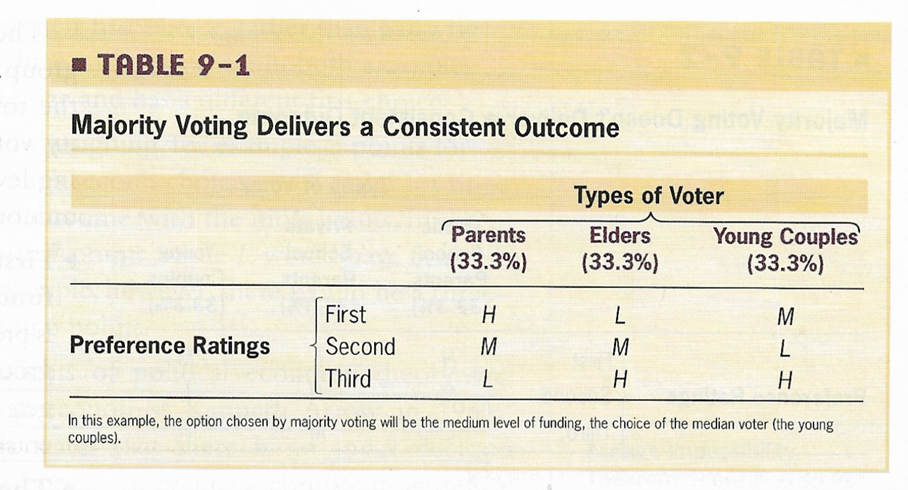
\includegraphics[width=0.7\linewidth]{Imagens/a14i2.png}
\end{figure}

Primeiro, vota-se entre H e L: \(\rightarrow\)L é preferido.

Segundo, vota-se entre H e M: \(\rightarrow\)M é preferido.

Finalmente, vota-se entre L e M: \(\rightarrow\)M é preferido.

Há escolha majoritária consistente: M.

Agora, troca-se o grupo dos idosos, por adultos (casais) que podem optar por colocar seus filhos em escolas privadas. 

\subsubsection{\textbf{Teorema de Impossibilidade de Arrow (1951)}}
\href{https://www.youtube.com/watch?v=849u239O5yo}{Vídeo}

Não há regra de decisão social (votação) que converta preferências individuais em decisões agregadas consistentes, a não ser que:\begin{itemize}
    \item O tipo de preferências individuais dos eleitores seja restringido (a aquelas que tenham um único ponto de máximo);
    \item A preferência de um ditador seja imposta à sociedade. 
\end{itemize}

\newpage
\section{\textbf{Teorema do Eleitor Mediano e Public Choice}}
\subsubsection{\textbf{Teorema de Impossibilidade de Arrow (1951)}}
\href{https://www.youtube.com/watch?v=849u239O5yo}{Vídeo}

Não há regra de decisão social (votação) que converta preferências individuais em decisões agregadas consistentes, a não ser que:\begin{itemize}
    \item O tipo de preferências individuais dos eleitores seja restringido (a aquelas que tenham um único ponto de máximo);
    \item A preferência de um ditador seja imposta à sociedade. 
\end{itemize}

\textbf{Outro modelo explicativo de decisões públicas por voto majoritário:}\begin{itemize}
    \item Teorema do Eleitor Mediano
\end{itemize}

\subsection{\textbf{Teorema do Eleitor Mediano}}
\textbf{O Teorema do Eleitor Mediano} afirma que a votação majoritária levará ao resultado preferido pelo eleitor mediano, que é o eleitor cuja preferência esteja no meio do grupo de eleitores: 50\% dos eleitores preferem mais, 50\% preferem menos. 

Aqui, não há necessidade de se conhecer os benefícios marginais derivados das políticas por cada um dos eleitores: somente o \textit{ranking} dos eleitores interessa. 

Suponha uma cidade com 1.001 eleitores e estão decidindo sobre a instalação de câmeras pela cidade para aumentar a segurança. Esta medida custaria \$40.040, o que implicaria um imposto adicional de \$40 por eleitor.
500 eleitores são muito favoráveis e estariam dispostos a pagar até \$100. Mas 501 acham a medida inócua e não querem pagar o imposto. O benefício social marginal da política será de 500 x 100 = 50.000 e o custo social marginal (preço) = 40.040, então seria eficiente implementar a política.  Mas não será, porque pela votação majoritária, a medida não será aprovada, dado que o eleitor mediano não é favorável à medida.  Resultado pelo eleitor mediano pode ser ineficiente (dependerá das intensidades das preferências dos eleitores). 

\subsection{\textbf{Teorema do Eleitor Mediano em Democracias Representativas}}
Representantes levam em conta as preferências do público e votam de acordo.

\textbf{Resultado}: os políticos eleitos escolhem o resultado que é preferido pelo eleitor mediano.

Hipótese aqui (e em toda a escola do \textit{public choice}): a única coisa que importa ao político eleito é maximizar os votos que ele(a) obtém nas eleições. \begin{itemize}
    \item \textbf{Resultado}: votará de acordo com o eleitor mediano (assumindo a hipótese de preferências com ponto máximo único).
\end{itemize} 

\subsection{\textbf{Preferências sobre Grau de Abertura da Economia}[Gruber, Cap.9 Figure 9-3]}
\begin{figure}[H]
    \centering
    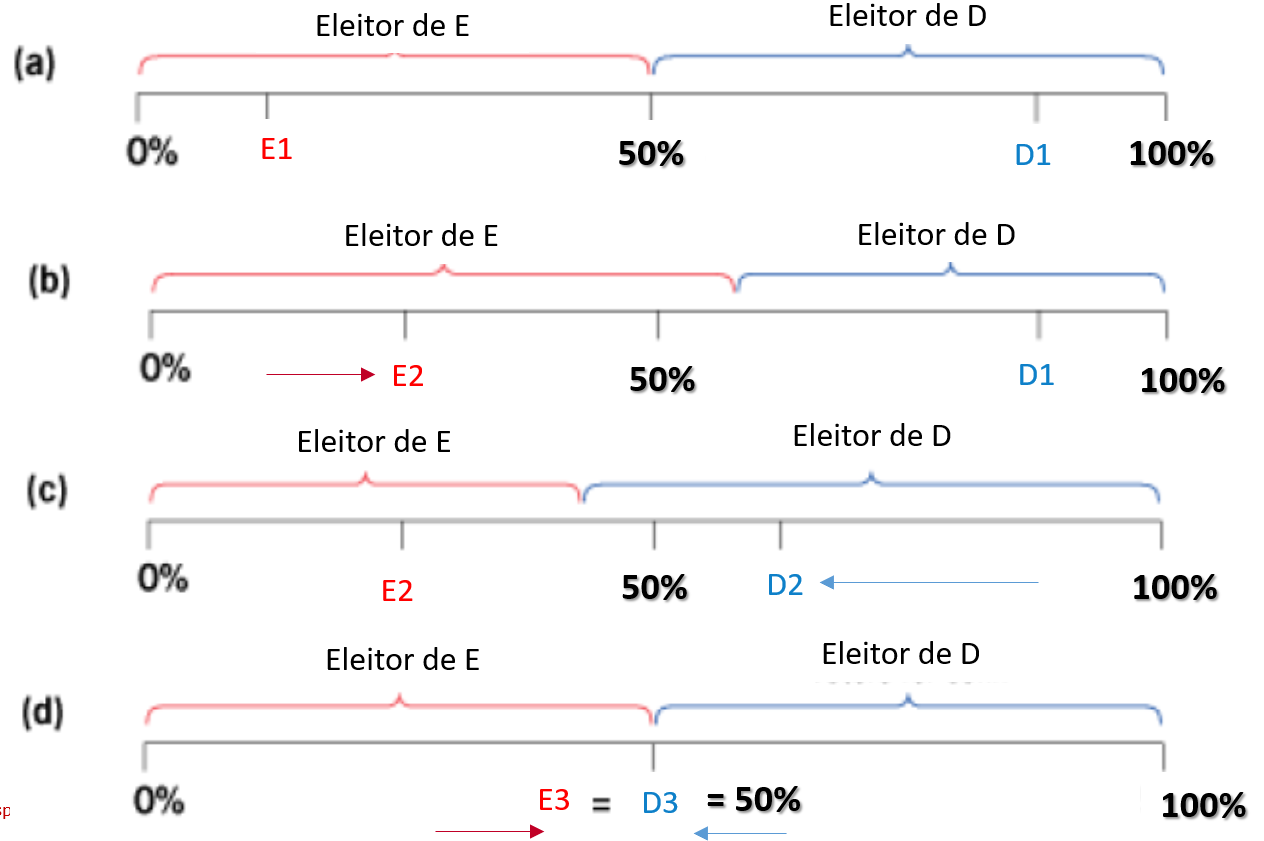
\includegraphics[width=0.7\linewidth]{Imagens/a15i1.png}
\end{figure}

\subsection{\textbf{Teorema do Eleitor Mediano: Hipóteses }}

Votação unidimensional de matérias:\begin{itemize} 
 \item mas pode haver matéria que seja mais consensual;
 \item também pode haver forte correlação de preferências entre as diferentes matérias.
\end{itemize}

Há somente dois candidatos/propostas.

Não há influência de ideologia.

Não há votação seletiva (todos votam). 

Não há influências financeiras na eleição.

Informação perfeita de políticos e eleitores sobre as matérias, e entre eles. 

\subsection{\textbf{Verdade???}}
\href{https://www.infomoney.com.br/politica/lula-tera-de-migrar-para-o-centro-diz-landau/}{Link 1}

\href{https://trademap.com.br/agencia/mercados/tanto-bolsonaro-quanto-lula-terao-que-migrar-para-o-centro-diz-ex-bc-luiz-fernando-figueiredo}{Link 2}

\subsection{\textbf{Teorema do Eleitor Mediano}}
\href{https://www.facebook.com/429608184068695/videos/389419731878556/UzpfSTEwNjE1NTYyMDY6MTAyMTYxMjM5NDU2NjU2NzY/}{Uma aula esclarecedora}

\textbf{Aos interessados}
\begin{figure}[H]
    \centering
    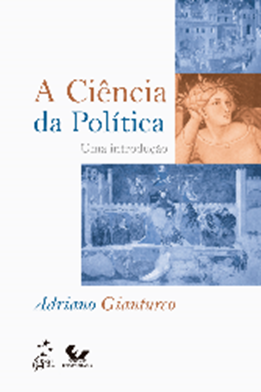
\includegraphics[width=0.7\linewidth]{Imagens/a15i2.png}
\end{figure}

\textbf{Funciona na prática?}\href{http://www.scielo.br/scielo.php?pid=S0034-71402006000300005&script=sci_arttext}{Provisão de bens públicos no Brasil}.

\begin{figure}[H]
    \centering
    \includegraphics[width=0.7\linewidth]{Imagens/a15i3.png}
\end{figure}

\subsection{\textbf{Conhecendo um pouco mais a teoria do Public Choice (Escolha Pública)...}}
\subsubsection{\textbf{Entendendo o “planejador central”}}
O objetivo nem sempre é maximizar o benefício social, mas é gerar transferências entre grupos particulares na sociedade. Muitas vezes, essas transferências são feitas de maneira ineficiente. 

Políticas públicas respondem a grupos de interesses: teoria da captura.

\begin{figure}[H]
    \centering
    \includegraphics[width=0.7\linewidth]{Imagens/a15i4.png}
\end{figure}
\textit{Stigler, G. J. (1971). “The theory of economic regulation”. The Bell journal of economics and management science, 3-21. Prêmio Nobel em Economia 1982}

Duas premissas:\begin{itemize}
    \item Recurso básico (e mais importante) do Estado: poder de coerção. Grupos de interesse podem convencer o estado a usar tal poder para aumentar seu próprio benefício.
    \item Agentes são racionais.
\end{itemize}

\textit{“We assume that political systems are rationally devised and rationally employed, which is to say that they are appropriate instruments for the fulfillment of desires of members of the society” (1971).}

\subsubsection{\textbf{Hipóteses}}
Agentes políticos são pessoas como todas as outras: \textbf{racionais, interessados e maximizadores.}\begin{itemize}
    \item Não quer dizer que são “maus” ou “corruptos” naturalmente. 
    \item Para chegar ao seu objetivo, precisam tomar o poder político e mantê-lo ao longo do tempo.
    \item Quando ficam aparentes os defeitos destes agentes, “vêm disfarçados de boas intenções sob rótulos os mais chamativos: ‘vontade geral, interesse público, políticas públicas para atender necessidades coletivas, princípios de eficiência, de segurança, de economia, [Justiça], etc.”
\end{itemize}

Individualismo metodológico: analisa-se o comportamento concreto dos agentes políticos (e não como deveriam idealmente ser).\begin{itemize}
    \item Quais incentivos recebem? (pouco importa os fins declarados)
    \item O que fazem realmente? (pouco importa o que deveriam fazer, ou o que dizem que querem fazer).
\end{itemize}

Não se vira um santo (ou herói) em política.\begin{itemize}
    \item Políticos também visam o lucro (lucro econômico e renda política). 
    \item Não são melhores ou piores do que outros agentes: procuram o próprio benefício antes do benefício dos outros. 
\end{itemize}

Falhas de Estado: Nem sempre o governo consegue, e nunca de maneira estrita, alcançar o resultado desejado. \begin{itemize}
    \item Política tem falhas porque é feita de pessoas, pessoas imperfeitas. 
    \item Em casos de falhas de mercado, quem vai intervir são essas pessoas...
    \item ... Levando-se isso em conta, talvez a justificativa para a intervenção reduza bastante.
\end{itemize}

\subsubsection{\textbf{Objetos de estudo do Public Choice}}
\begin{figure}[H]
    \centering
    \includegraphics[width=0.7\linewidth]{Imagens/a15i5.png}
\end{figure}

\subsubsection{\textbf{Political business cycle}}
Literatura científica mostra que os ciclos econômicos (de \textit{boom} e \textit{bust}) tem forte correção com ciclos eleitorais.\begin{itemize}
    \item Ciclos econômicos teriam menos a ver com crises intrínsecas e inevitáveis do capitalismo. 
    \item Evidências do comportamento racional dos políticos, com vistas a garantir manutenção do poder. 
    \item Políticos têm incentivo a olhar a curto prazo, baseando-se na duração do próprio mandato.
    \item Ter eleições regularmente pode ser economicamente negativo. 
\end{itemize}

\subsubsection{\textbf{Benefícios concentrados e custos difusos}}
\begin{figure}[H]
    \centering
    \includegraphics[width=0.7\linewidth]{Imagens/a15i6.png}
\end{figure}

Ou benefícios difusos e custos concentrados...

Em ambos os casos, o  payoff concentrado pode ser o que vai motivar os movimentos políticos. \begin{itemize}
    \item Mesmo havendo motivação racional, mudanças que geram benefícios maiores podem não acontecer por dificuldade de organizar a ação coletiva:
    \item “A lógica da Ação Coletiva” (Mancur Olson.)
\end{itemize}

Explica também “bandeiras eleitorais”: pork barrel system.

\subsubsection{\textbf{Os Votantes*}}
Cada votante tem suas ideias, ideologia, preferências, interesses e necessidades. 

Também são autointeressados e sofrem de assimetria de informação – em comparação a todos os outros agentes da pirâmide política e entre eles (nada a ver com escolaridade). 

Votantes são míopes e se esquecem do passado (vários exemplos, i.e. Churchill).

Votantes têm ignorância racional.

Não votar é racional! 

\begin{figure}[H]
    \centering
    \includegraphics[width=0.7\linewidth]{Imagens/a15i7.png}
\end{figure}

\textit{“depois de estudar a opinião pública, você se pergunta como é possível que as democracias não gerem políticas ainda piores”} [Bryan Caplan]

\begin{figure}[H]
    \centering
    \includegraphics[width=0.7\linewidth]{Imagens/a15i8.png}
\end{figure}

\textit{“O melhor argumento contra a democracia é uma conversa de cinco minutos com o votante médio”.} [Winston Churchill]

\newpage
\section{\textbf{Previdência}}
\subsection{\textbf{Nas aulas passadas}}
Analisamos a provisão de bens públicos e bens com fortes falhas de mercado.\begin{itemize}
    \item Concluímos que, normalmente, o Estado deverá prove-los.
\end{itemize}

 Analisamos processos de agregação de preferências sociais em sistemas democráticos.\begin{itemize}
    \item Teorema de Impossibilidade de Arrow.
    \item Regras de maioria e tendências de equilíbrio (por ex. Teorema do Eleitor Mediano, entre outros). 
\end{itemize}

 Vimos como nem sempre (ou quase nunca) o Estado oferece esses bens e políticas como um “planejador central benevolente”. \begin{itemize}
    \item Agentes políticos pela visão do public choice (Teoria da captura, lobbies de minorias, etc.)
\end{itemize}

\subsection{\textbf{Três políticas públicas que estudaremos}}
Agora, vamos estudar 3 políticas públicas que viriam de preferências sociais (como várias outras políticas):\begin{itemize}
    \item Sistemas de Previdência
    \item Sistema Tributário
    \item Segurança Pública
\end{itemize}

\begin{figure}[H]
    \centering
    \includegraphics[width=0.7\linewidth]{Imagens/a16i1.png}
\end{figure}

\begin{figure}[H]
    \centering
    \includegraphics[width=0.7\linewidth]{Imagens/a16i2.png}
\end{figure}

\subsection{\textbf{Por que sistemas de previdência? Para quê sistemas de previdência?O Modelo do Ciclo de Vida e Suavização do Consumo(Base: Romer, 2001, Cap. 7)}}

\subsubsection{\textbf{Modelo do ciclo de vida e suavização do consumo: Ideia Principal}}

Dado o princípio da utilidade marginal decrescente, indivíduos preferem suavizar o consumo ao longo do tempo:\begin{itemize}
    \item Entre um ano de super-consumo e outro de grande escassez e dois anos seguidos de consumo médio, a preferência é por este segundo.
\end{itemize}

Assumindo um indivíduo que vive por T períodos e cuja utilidade da vida inteira é dada por:
\[
U=\sum_{t=1}^T u(C_t), \quad u'(\cdot)>0 \ \ e \ \ u''(\cdot)<0
\]

\(u(\cdot)\)é a função de utilidade instantânea; \(C_t\) é consumo em \(t\); Indivíduo tem riqueza inicial \(A_0\) e rendas de trabalho \(Y_1 \ \ ,\ \ Y_2 \ \ , \cdots \ ,Y_T \).Pode poupar ou tomar emprestado a uma taxa de juros exógena, mas não há Ponzi game (paga tudo ao fim da vida); assumimos taxa de juros e taxa de desconto intertemporal igual a 0.

A restrição orçamentária do indivíduo é:
\[
\sum_{t=1}^{T} c_t \leq A_0 + \sum_{t=1}^{T} y_t
\]

Utilidade marginal do consumo é sempre positiva, então a restrição é satisfeita com igualdade.

O Lagrangeano para o problema de maximização é:
\[
\mathcal{L} = \sum_{t=1}^{T} u(C_t) + \lambda \left( A_0 + \sum_{t=1}^{T} y_t - \sum_{t=1}^{T} c_t \right)
\]

A condição de primeira ordem para \( C_t \) é:
\[
u'(C_t) = \lambda
\]

Esta condição vale para todos os períodos:\begin{itemize}
    \item \(UMg\) é constante para cada \(t\).
\end{itemize}

Se \( \text{UMg} \) é constante para cada \( t \), e se é dada unicamente pelo consumo, então \( C \) deve ser constante: \(C_1 = C_2 = \cdots = C_t\)

Substituindo na restrição orçamentária para encontrar \( C_t \):
\[
\sum_{t=1}^{T} C_t \leq A_0 + \sum_{t=1}^{T} y_t
\]

\[
C_t = \underbrace{\frac{1}{T} \underbrace{\left( A_0 + \sum_{t=1}^{T} Y_t \right)}_{\text{Recursos obtidos durante a vida.}}}_\text{Renda permanente (Milton Friedman)} \quad \text{para todo } t
\]

O indivíduo divide o total de seus recursos obtidos ao longo da vida, igualmente, para o consumo em cada período.

O consumo em cada período não é dado pelo nível de renda daquele período, mas pela expressão à direita da equação acima, que Friedman (1957) chamou de \textbf{renda permanente}(divido a utilidade marginal constante).

A diferença entre a renda corrente e a renda permanente é a \textbf{renda transitória}.

\textbf{Efeitos críticos para a poupança:}

\[
S_t = Y_t - C_t
\]

\[
S_t = \underbrace{\left( Y_t - \overbrace{\frac{1}{T} \sum_{t=1}^{T} Y_t}^{C_t} \right) - \frac{1}{T} A_0}_\text{Renda transitória : Poupança em cada um dos perídos} 
\]

Poupança será alta quando a renda em \( t \) for maior que a média, ou seja, quando a renda transitória for alta.

Vice-versa para períodos \( t \) em que a renda transitória for abaixo da renda permanente: poupança negativa.

\textbf{O indivíduo usa poupança e dívida (poupança negativa) para suavizar a trajetória de consumo.}

Ideia principal da hipótese do ciclo de vida e da renda permanente de Modigliani \& Brumberg (1954) e Friedman (1957). 

\begin{figure}[H]
    \centering
    \includegraphics[width=0.25\linewidth]{Imagens/a16i3.png}
\end{figure}
\begin{figure}[H]
    \centering
    \includegraphics[width=0.25\linewidth]{Imagens/a16i4.png}
\end{figure}

\begin{figure}[H]
    \centering
    \includegraphics[width=0.6\linewidth]{Imagens/a16i5.png}
\end{figure}

Mas... ao longo da vida, os indivíduos têm, normalmente:\begin{itemize}
    \item incertezas sobre suas receitas (acidentes, fatos inesperados, mudanças de rumos, etc.);
    \item capacidades diferenciadas de geração de receita. 
    \item Suavização do consumo afetada. 
\end{itemize}

Problema: apesar de preferir a \textbf{suavização do consumo} existe \textbf{comportamento míope} das pessoas no geral (incertezas, racionalidade limitada, longo prazo, etc.) que leva à poupança negativa durante a juventude. 

Além disso, existem informações assimétricas no mercado de seguros, levando à \href{https://www.aeaweb.org/research/stopping-the-death-spiral}{seleção adversa} e tornando a oferta privada ineficiente.

Para isso, o estado precisa prover \textbf{sistemas públicos de seguridade social (previdência + assistência).}

\subsection{\textbf{O Sistema Previdenciário Brasileiro}}

Luís Eduardo Afonso (2005) \textit{in Arvate e Biderman, “Economia do Setor Público no Brasil”} 

\subsubsection{\textbf{Seguridade social}}

No Brasil, o Instituto Nacional do Seguro Social (INSS) é o principal provedor de todos os programas de seguridade social.

Programas incluídos:\begin{itemize}
    \item Aposentadoria (todos os tipos)
    \item Pensão (Por isso casamento é um contrato)
    \item Auxílio-acidente
    \item Auxílio-doença
    \item \href{https://www.inss.gov.br/beneficios/}{Mais...}
\end{itemize}

Seguridade social = previdência + assistência.

\subsubsection{\textbf{Sistema de Repartição (pay as you go) e Sistema de Capitalização}}

\textbf{Regime de Repartição}: as contribuições dos trabalhadores no período t são utilizadas no mesmo período para o pagamento das aposentadorias dos inativos daquele período. \begin{itemize}
    \item Solidariedade intergeracional (mas obrigatório).
    \item Maioria dos países adota em alguma medida: processo histórico de escolha, com base em condições econômicas e demográficas.
\end{itemize}

Samuelson(1958) e Diamond(1965): a taxa de retorno implícita a um regime de repartição pode ser expressa: \begin{itemize}
    \item \(1 + r = (1 + w) (1 + n)\)
    \item \(r\): taxa de retorno da previdência social = iguala fluxo de valores presentes das contribuições e o fluxo de benefícios.
    \item \(w\): taxa de crescimento salarial (vem da economia). Vem da produtividade marginal do trabalho \(PMg_T\)
    \item \(n\): taxa de crescimento populacional.
\end{itemize}

Taxa de retorno e valor da aposentadoria de cada geração são função de fatores econômicos, demográficos e tecnológicos. 

\textbf{Regime de Capitalização:} as contribuições de cada indivíduo são aplicadas e capitalizadas a cada período, visando formar um fundo que custeará sua própria aposentadoria.

O valor da aposentadoria é função direta do montante contribuído pelo indivíduo durante a vida ativa e da taxa de juros que remunera o fundo (taxa de juros da economia). 

Baixa liquidez do fundo; não existe solidariedade intergeracional. 

Parâmetros previdenciários (expectativa de vida, alíquota de contribuição, taxa de juros, duração da vida ativa) deve levar a VP de contribuições que seja igual ao VP dos benefícios. \(\rightarrow\) regime atuarialmente "justo".

\subsection{\textbf{Efeitos Redistributivos do Atual Sistema de Previdência Brasileiro (baseado em regime de repartição)}}

\subsubsection{\textbf{Aspectos (re)distributivos: Inter e Intragerações}}

Como discutido longamente em Tafner e Giambiagi, 2011 – que leremos ainda.

\subsubsection{\textbf{Aspectos (re)distributivos: Gênero}}

“Como as mulheres têm maior expectativa de vida que os homens, é esperado que (inexistindo diferença nas datas de entrada e saída do mercado de trabalho) recebam benefícios previdenciários por um período maior. Logo, qualquer regime que assegure a homens e mulheres, ceteris paribus, aposentadorias com idades iguais, \textbf{estará transferindo renda do grupo masculino para o feminino, dentro de uma mesma geração”} (p.387).

E no Brasil, há ainda benefícios previdenciários que largamente favorecem mais as mulheres do que os homens (ex.: pensões por morte, salário maternidade, etc). 

\subsubsection{\textbf{Aspectos (re)distributivos: Rural x Urbano}}

\begin{figure}[H]
    \centering
    \includegraphics[width=0.7\linewidth]{Imagens/a17i1.png}
\end{figure}

\subsubsection{\textbf{Aspectos (re)distributivos: Setor público x Setor privado}}
Regras mais generosas aos servidores públicos, que tinham aposentadorias integrais  (até a reforma de 2003), dura mais tempo sendo regressivo.

Em 2001, o déficit do sistema previdenciário do setor público respondia por 79.2\% do déficit total da previdência (sendo o número de aposentados e pensionistas públicos muito menor do que no setor privado, cerca de 13\%). [Dados mais atualizados em TG, 2011, Tab.2].

\begin{figure}[H]
    \centering
    \includegraphics[width=0.7\linewidth]{Imagens/a17i2.png}
\end{figure}

\begin{figure}[H]
    \centering
    \includegraphics[width=0.7\linewidth]{Imagens/a17i3.png}
\end{figure}

\subsection{\textbf{Atividade Prática}}

Analise a página do Insper com dados sobre a Previdência às vésperas da Reforma de 2019. \begin{itemize}
    \item Cite 5 dos problemas e explique porquê eles tendem a piorar o déficit da previdência brasileira.
    \item Responda: há alguma “anomalia” do sistema brasileiro em comparação a de outros países?
    \item Pode ser feito em grupo de até 3 pessoas. (Entregar para mim.)
    \item \href{https://www.insper.edu.br/conhecimento/conjuntura-economica/reforma-previdencia-brasil-em-graficos/}{Insper}
\end{itemize}

\newpage
\section{\textbf{Tributação e Sistema Tributário}}
\href{https://www.youtube.com/watch?v=fQ0t_BuXIrU}{O que o imposto faz com alguém}

\begin{figure}[H]
    \centering
    \includegraphics[width=0.7\linewidth]{Imagens/a18i1.png}
\end{figure}

\begin{figure}[H]
    \centering
    \includegraphics[width=0.7\linewidth]{Imagens/a18i2.png}
\end{figure}

\subsection{\textbf{Alguns Indicadores}}
\textbf{Nacionais:} \url{http://www.impostometro.com.br/}

\textbf{Internacionais:} \url{https://archive.doingbusiness.org/en/data/exploreeconomies/brazil}

\subsection{\textbf{Doing Business (2020) e Outros Indicadores}}
\begin{figure}[H]
    \centering
    \includegraphics[width=0.7\linewidth]{Imagens/a18i3.png}
\end{figure}

\begin{figure}[H]
    \centering
    \includegraphics[width=0.5\linewidth]{Imagens/a18i4.png}
\end{figure}

\begin{figure}[H]
    \centering
    \includegraphics[width=0.5\linewidth]{Imagens/a18i5.png}
\end{figure}

\begin{figure}[H]
    \centering
    \includegraphics[width=0.7\linewidth]{Imagens/a18i6.png}
\end{figure}

\subsection{\textbf{“Imposto é roubo!” (?)}}
Solução em casos de falhas de mercado:
\begin{itemize}
  \item Externalidades negativas;
  \item Externalidades positivas;
  \item Assimetrias de informação (por exemplo, sistemas de previdência);
  \item Provisão de bens públicos, etc.
\end{itemize}

Politicamente e socialmente, é a contrapartida do ``Contrato Social'':
\begin{itemize}
  \item Custeio da máquina estatal (provisão de bens públicos);
  \item ``Justiça'', igualdade e redistribuição de renda na sociedade (Segundo Teorema de Bem-Estar).
\end{itemize}


\subsection{\textbf{Princípios de um sistema tributário ótimo}}

Os indivíduos devem contribuir na proporção de suas capacidades de pagamento ou rendimentos. \textbf{[Progressividade]}.

Todo tributo deve ser arrecadado de forma que implique o menor custo possível para o contribuinte além do valor arrecadado pelo Estado (ou seja, minimizar peso morto da sociedade) \textbf{[Eficiência]}.

O tributo a ser pago deve ser certo e não arbitrário, com valor a ser pago e forma do pagamento claros e evidentes para o contribuinte.\textbf{ [Transparência, não- arbitrariedade]}.

Todo tributo deve ser arrecadado de maneira mais conveniente para o contribuinte.

\subsection{\textbf{Tributos e distorções no comportamento}}

Tributos causam \textit{distorções}, por definição, pois induzem os indivíduos a se comportarem de determinada maneira $\Rightarrow$ peso morto.

Para não causar distorções na escolha das pessoas, tributo deveria ser \textit{lump sum}: montantes fixos de dinheiro que as pessoas pagam ou recebem independente de suas escolhas.
\begin{itemize}
  \item Exemplo: imposto per capita, imposto baseado em características pessoais inalteráveis, etc.
  \item Difícil conseguir tais informações.
\end{itemize}

Todos os outros tributos causam distorções (peso morto).


\subsection{\textbf{Relembrando de Micro 1...}}
\subsubsection{\textbf{Efeitos de Impostos no Equilíbrio Competitivo}}
\begin{figure}[H]
    \centering
    \includegraphics[width=0.7\linewidth]{Imagens/a18i7.png}
\end{figure}

\begin{figure}[H]
    \centering
    \includegraphics[width=0.7\linewidth]{Imagens/a18i8.png}
\end{figure}

\subsection{\textbf{Progressividade x Regressividade}}
\textbf{Princípio da equidade horizontal:}
\begin{itemize}
  \item ``Pessoas similares, devem pagar tributos similares mesmo se fazem escolhas diferentes; ou, pessoas similares não devem pagar tributos diferentes por situações causadas por motivos aleatórios''.
\end{itemize}

\textbf{Princípio da equidade vertical:}
\begin{itemize}
  \item ``Pessoas com mais recursos devem pagar mais tributos do que pessoas com menos recursos'';
  \item Distribuição de renda (não-concentração) na sociedade: função de bem estar social onde a redistribuição ocorre de grupos com menor UMgC para aqueles com maior UMgC;
  \item (``Princípio da Isonomia/Igualdade: tratar igualmente os iguais e desigualmente os desiguais na medida de sua desigualdade'');
  \item Senso de ``Justiça'' Aristotélica).
\end{itemize}

Para alcançar a equidade vertical, o tributo precisa ser progressivo: a alíquota média/efetiva (a porcentagem da renda total paga no imposto) precisa aumentar mais que proporcionalmente com o aumento da renda (ricos pagam parcela maior de suas rendas do que pobres).

Tributos ou sistemas em que a alíquota média não muda com a renda são tributos proporcionais: todos pagam a mesma proporção da renda com o imposto(s).

Tributos ou sistemas em que a alíquota média cai com a renda são regressivos.

Como é no Brasil?\href{http://idg.receita.fazenda.gov.br/acesso-rapido/tributos/irpf-imposto-de-renda-pessoa-fisica#c-lculo-anual-do-irpf}{Link Brasil}

\subsection{\textbf{Tributo direto x Tributo indireto}}
\textbf{Tributo direto:} o ônus do tributo é assumido direta e integralmente pelo contribuinte (ex.IR).

\textbf{Tributo indireto:} o ônus pode ser repassado para outro agente econômico via preços de mercado (ex.: ICMS, IPI, etc.)

(Tem a ver com \textbf{incidência  tributária}, que veremos em aulas futuras.)

\subsection{\textbf{Progressividade e Regressividade, Tributos Diretos e Indiretos}}
\begin{figure}[H]
    \centering
    \includegraphics[width=0.7\linewidth]{Imagens/a18i9.png}
\end{figure}

\begin{figure}[H]
    \centering
    \includegraphics[width=0.7\linewidth]{Imagens/a18i10.png}
\end{figure}

\subsection{\textbf{Regressividade do tributo sobre consumo}}
\begin{figure}[H]
    \centering
    \includegraphics[width=0.7\linewidth]{Imagens/a18i11.png}
\end{figure}

\subsection{\textbf{Tributação Ótima: Regra de Ramsey}}
Frank Ramsey: como um governo pode arrecadar uma receita fiscal R, criando o menor peso morto possível? Como estabelecer as alíquotas de impostos entre diferentes mercadorias?

O governo deve estabelecer alíquotas de forma que a razão entre o peso morto marginal e a receita marginal gerada por cada mercadoria seja igual entre todas elas.

Fixar tributos de forma que:
\[
\frac{Peso\ Morto\ Marginal_i}{Receita\ Marginal\ do\ Tributo_i} = \lambda
\]

$\lambda$ igual para todos as mercadorias.

\textbf{Peso Morto Marginal de ``i'':}
\begin{itemize}
  \item Custo marginal ao consumidor pelo aumento do tributo sobre ``i'';
  \item É função crescente da alíquota do tributo.
\end{itemize}

Na prática, não há medida clara do valor de $\lambda$; usada em discussões sobre reforma tributária.

No entanto, em mercados de oferta competitiva, a regra de Ramsey implica* que a alíquota de imposto ótima para ``i'' seja:
\[
\tau_i^* = -\frac{1}{\eta_i} \times \lambda \quad \text{\small {Regra do Inverso da Elasticidade}}
\]

$\eta_i$ é a elasticidade de demanda de ``i''.

\textbf{Implicações:}
\begin{enumerate}
  \item[\textbf{i.}] O governo deveria taxar de maneira \textbf{inversamente proporcional à elasticidade} da mercadoria: alíquota maior para mercadorias menos elásticas, e vice-versa**.
  \item[\textbf{ii.}] Deve criar um sistema tributário com \textbf{ampla base de tributação, de alíquotas menores}, do que base restrita e alíquotas altas**.
\end{enumerate}

\subsection{\textbf{Tributo sobre Renda: Curva de Laffer}}
\begin{figure}
    \centering
    \includegraphics[width=0.75\linewidth]{Imagens/a18i12.png}
\end{figure}

\begin{figure}[H]
    \centering
    \includegraphics[width=0.7\linewidth]{Imagens/a18i13.png}
\end{figure}

\begin{figure}[H]
    \centering
    \includegraphics[width=0.7\linewidth]{Imagens/a18i14.png}
\end{figure}

\begin{figure}[H]
    \centering
    \includegraphics[width=0.7\linewidth]{Imagens/a18i15.png}
\end{figure}

\href{https://www.federalreserve.gov/pubs/ifdp/2012/1048/ifdp1048.pdf}{Curvas de Laffer de IR de Diversos Países}

\begin{figure}[H]
    \centering
    \includegraphics[width=0.7\linewidth]{Imagens/a18i16.png}
\end{figure}

\href{https://www.reddit.com/r/dataisbeautiful/comments/7mvec3/laffer_curves_for_27_oecd_countries/}{Mais}

\href{https://www.federalreserve.gov/pubs/ifdp/2012/1048/ifdp1048.pdf}{Curva de Laffer de diferentes tributações em alguns países (estudo do Federal Reserve).}

\newpage
\section{\textbf{Economia do Crime}}
\subsection{\textbf{Motivações do último capítulo do semestre}}
O crime compensa?
  \begin{itemize}
    \item De quanto em comparação com o salário médio brasileiro?
  \end{itemize}
Só prisão ``pune''? Por que não penas ``alternativas''?

Legalizar drogas é ``uma boa''?

O que os \textbf{dados} dizem afinal: facilitar porte de armas gera mais ou menos mortes?
                    
\begin{center}
\textbf{VAMOS RESPONDER CIENTIFICAMENTE A ESSAS QUESTÕES!! (COM A CIÊNCIA ECONÔMICA!)}
\end{center}

\subsection{\textbf{Vamos começar trabalhando hoje…}}
Leiam (somente leiam):\href{https://veja.abril.com.br/coluna/direito-e-economia/o-crime-compensa-no-brasil-perguntem-aos-proprios-criminosos/}{link}

\subsection{\textbf{Motivações iniciais}}

Shikida (2010): \textbf{apenas 2\% dos criminosos efetivamente ``pagam pelo crime''} sendo encarcerados na cadeia.

Ehrlich (1975): uma \textbf{execução de pena capital} a mais por ano reduz o número de \textbf{homicídios} em \textbf{7 ou 8} (por ano).

Os custos envolvidos num processo que resulta em pena capital (\textit{pena de morte}) \textbf{estão estimados em US\$ 2 milhões, por caso}.

Donohue \& Levitt (2001) explicam a queda na criminalidade dos EUA nos anos 90 pela \textbf{legalização do aborto}.

\href{https://alinsperedu-my.sharepoint.com/personal/hichamt_al_insper_edu_br/Documents/Insper/Período%206/Direito%20e%20Economia%20das%20Políticas%20Públicas/Materiais%20e%20Aulas%20PPT/LSE-IDEAS-DRUGS-REPORT-FINAL-WEB.pdf}{Grupo de Especialistas da LSE (London School of Economics)} (2014): as políticas nacionais e supranacionais de combate ao tráfico de drogas foram um tremendo fracasso.
\begin{itemize}
  \item Políticas eficientes deveriam focar na descriminalização deste mercado.
\end{itemize}

Em média, 66\% dos crimes no Brasil não são reportados (Caetano, Garcia, Yeung e Ghiggi, 2020).

\begin{figure}[H]
    \centering
    \includegraphics[width=0.7\linewidth]{Imagens/a19.1.png}
\end{figure}

Outros assuntos na Economia do Crime atual:
\begin{itemize}
  \item Redução da maioridade penal como estratégia para reduzir crimes.
  \item Descriminalização de drogas.
  \item Impactos do porte de armas legalizado.
  \item Leis de combate ao crime mais/menos rigorosas e impacto na redução de crimes.
  \item \dots
\end{itemize}

\subsection{\textbf{O pai de tudo…}}
\begin{figure}[H]
    \centering
    \includegraphics[width=0.7\linewidth]{Imagens/a19i2.png}
\end{figure}
“‘Crime’ is an economically important activity or ‘industry’, notwithstanding the almost  total neglect by economists…”
\textbf{\textit{Gary Becker (1968)}}

(\textbf{\textit{Felizmente}}) Muita coisa mudou desde então...

\subsection{\textbf{Teoria Econômica do Crime}}
\textbf{Objetivos}\begin{itemize}
    \item Apresentar um modelo de previsão do comportamento criminal (decisão micro).
    \item Fazer previsões dos efeitos de políticas de prevenção do crime (decisão macro).
\end{itemize}

\textbf{\textit{Observação}}: Estamos estudando o modelo originalmente proposto por Becker (1968), mas adaptado por Cooter e Ulen (2010).

Não esquecer!

Teoria de Becker analisa:
\begin{itemize}
  \item Decisão microeconômica do criminoso e também a decisão ``macroeconômica'' de políticas públicas – completamente diferentes!
  \item Resultado micro e resultado macro no ``mercado de crimes''.
\end{itemize}

\subsubsection{\textbf{Consequências Individuais da Racionalidade do Crime (análise micro)}}
Vamos considerar um agente \textit{amoral} e racional.

Vamos ver o gráfico relacionando punição com gravidade do crime (todos padronizados em valores monetários).

A punição será maior quanto mais grave for o crime.

Exemplo: Crime econômico (corrupção, crime financeiro, furto, assalto de bens, etc.)

\begin{itemize}
  \item Indenização perfeita não é suficiente para deter o crime?
\end{itemize}

Não, porque a punição é probabilística:

\begin{equation*}
\mathit{VE\ Crime = Ganhos - (valor\ da\ punição \times \textit{prob. de ser pego e punido})^\#}
\end{equation*}

\textbf{Notações:}
\begin{itemize}
  \item $x$: tamanho do crime (em \$)
  \item $y$: ganho do criminoso em cometer o crime
  \item $f$: punição (em \$)
  \item $p$: probabilidade de cometer um crime e ser preso
  \begin{itemize}
    \item $y = y(x)$; $f = f(x)$; $p = p(x)$
    \item $y = y(x)$ e $f = f(x)$ são \textit{crescente}s
    \item E $p = p(x)$?
  \end{itemize}
\end{itemize}

\textbf{Valor esperado da punição} = $f(x) \cdot p(x)$

\textit{ PS: Essa equação \textbf{não é exatamente} a função de Becker.}

O criminoso racional, amoral, maximizará seu \textit{payoff} líquido:
\[
\max_{x} \; y(x) - p(x) \cdot f(x)
\]
\begin{figure}[H]
    \centering
    \includegraphics[width=0.7\linewidth]{Imagens/a19i3.png}
\end{figure}

O criminoso maximizará seu \textit{payoff} onde BMg de uma ``unidade adicional'' de crime iguale o CMgE da punição:
\[
y' = p'f + pf'
\]

As derivadas indicam o aumento dos valores para mudanças marginais em $x$.

$f'$ é positivo. Por quê?

$p'$ também é (pode ser) positivo. Por quê?

Como pode ser enxergado o “lucro” do crime? 

Onde será o lucro máximo?

Como observar CMg e BMg?

Qual será a decisão do criminoso racional?

\textbf{Podemos ajustar o modelo para a decisão agregada (“social”) do crime...}

\subsubsection{\textbf{Consequências no Mercado da Racionalidade do Crime}}
Com uma pequena mudança, podemos ajustar o modelo acima de gravidade para quantidade de crimes cometidos.

Passamos a uma curva onde o número de crimes decresce à medida que o valor esperado da punição aumenta.

É uma “curva de oferta (ou demanda) agregada” por crime.

\begin{figure}[H]
    \centering
    \includegraphics[width=0.7\linewidth]{Imagens/a19i4.png}
\end{figure}

\begin{figure}[H]
    \centering
    \includegraphics[width=0.7\linewidth]{Imagens/a19i5.png}
\end{figure}

As Equações de Becker (1968)\begin{itemize}
    \item A decisão individual:
    \item Esta abordagem implica que existe uma função que relaciona o número de delitos cometidos por um indivíduo com sua probabilidade de condenação, sua punição se condenado e outras variáveis, como a renda disponível em atividades legais e ilegais, a frequência de detenções menores e sua disposição para cometer um ato ilegal. Isso pode ser representado como:
    \[
    O_j = O_j(p_j, f_j, u_j),
    \]
    \item onde: 
    \begin{itemize}
        \item $O_j$ é o número de delitos cometidos por $j$ durante um determinado período;
        \item $p_j$ é a probabilidade de condenação por delito;
        \item $f_j$ é a punição por delito;
        \item $u_j$ é uma variável guarda-chuva representando todas as demais influências.
    \end{itemize}
\end{itemize}

\subsubsection{\textbf{A Matemática do crime racional}}
Como o gráfico mudaria se a polícia for mais eficiente e conseguir capturar uma maior quantidade de criminosos?

Como o gráfico mudaria de forma a refletir mudança no comportamento criminal?

\begin{figure}[H]
    \centering
    \includegraphics[width=0.7\linewidth]{Imagens/a19i6.png}
\end{figure}

\begin{figure}[H]
    \centering
    \includegraphics[width=0.7\linewidth]{Imagens/a19i7.png}
\end{figure}

\textbf{As curvas podem ter outros formatos???}

\subsubsection{\textbf{Efeitos da incerteza da punição}}

\begin{figure}[H]
    \centering
    \includegraphics[width=0.75\linewidth]{Imagens/a19i8.png}
\end{figure}

Pode-se também aumentar o custo de oportunidade de se cometer um crime que leve à redução de y’, ou seja, o BMg de aumentar a gravidade do crime. 

\textbf{Mudanças na probabilidade de punição, severidade da punição e oportunidades de engajar em crime levam a mudanças no comportamento criminal.}

\subsubsection{\textbf{A Matemática do crime racional}}
\textbf{Conclusões Importantes}
\begin{itemize}
    \item Aumentar fiscalização aumenta $p'$, que aumenta $CMg$;
    \item Aumentar o sistema de punições aumenta $f'$, que também aumenta $CMg$;
    \item Resultado de ambas medidas: reduzir gravidade (em \$) dos crimes.
\end{itemize}

\subsection{\textbf{Da decisão individual para a decisão de políticas públicas (análise macro) : discussão em Becker (1968)}}

\subsubsection{\textbf{A decisão do policy maker}}
O objetivo é criminalidade zero?

\subsubsection{\textbf{Voltando a Becker(1968)...}}
A perda social total é representada por:

\[
L = L(D, C, bf, O)
\]

Essa função mede a perda social, presumivelmente com:

\[
\frac{\partial L}{\partial D} > 0, \quad \frac{\partial L}{\partial C} > 0, \quad \frac{\partial L}{\partial bf} > 0
\]

O objetivo é selecionar valores de $f$, $C$ e possivelmente $b$ que minimizem $L$.

Assume-se que a função de perda seja idêntica à perda social total em termos de renda real advinda de crimes, condenações e punições:

\[
L = D(O) + C(p, O) + bpfO
\]

Onde:
\begin{itemize}
    \item $D(O)$: número de delitos cometidos (offenses);
    \item $C(p, O)$: custo de combate aos crimes (prevenção), função da probabilidade de punição $p$ e do número de crimes $O$;
    \item $bf$: perda por crime punido;
    \item $pO$: número de crimes punidos (probabilidade $\times$ número de delitos).
\end{itemize}

O resultado ótimo para a sociedade (minimização de custos) dependerá se o agente criminoso médio é avesso, neutro ou propenso ao risco.

Sendo neutros aos risco, p e f se compensam perfeitamente.\begin{itemize}
    \item Resultado Ótimo: p tendendo a 0 e f muito alto.
\end{itemize}

\subsubsection{\textbf{Quantidade ótima de prevenção do crime}}
\begin{figure}[H]
    \centering
    \includegraphics[width=0.7\linewidth]{Imagens/a20i1.png}
\end{figure}

\subsubsection{\textbf{Como mudaria a equação vista se formos levar em conta...}}
\begin{enumerate}
    \item ... que pessoas com emprego, maior salário, mais escolaridade, família, etc, tendem a cometer menos crime do que pessoas sem esses elementos (mantendo-se o tipo ou tamanho de crime contante)?
    \item ... a propensão ou aversão ao risco das pessoas ao cometer crime? 
    \item ... o fato de jovens serem mais “inconsequentes”, ou seja, mais imediatistas?
    \item ... que nem sempre o crime planejado dá certo?
    \item ... que o sistema judicial brasileiro é muito moroso e demora para condenar e executar uma pena? (vide Lava Jato)
    \item ... que ao longo do processo até a punição existem chances de subornar autoridades para não ser punido?
\end{enumerate}


\newpage
\section{\textbf{Estudos Dirigidos}}
\subsection{\textbf{1º Estudo Dirigido: Por que as Nações Falham; Capítulo 5 – Vi o Futuro e Funciona: O Crescimento num Contexto de Instituições Extrativas}}

O capítulo 5 de *Por que as Nações Falham*, de Daron Acemoglu e James Robinson, aborda a complexa relação entre crescimento econômico e instituições extrativas. Tradicionalmente, acredita-se que instituições extrativas sejam incapazes de promover o desenvolvimento sustentável, pois concentram poder e riqueza em uma elite, restringindo a inovação e a participação econômica. No entanto, os autores demonstram que, em algumas circunstâncias, sociedades com instituições extrativas podem experimentar crescimento econômico significativo, ainda que temporário e insustentável a longo prazo.

O crescimento sob instituições extrativas ocorre porque, para que uma elite possa extrair riquezas, ela precisa estimular algum nível de produção econômica. Governos autoritários ou centralizados podem criar um ambiente relativamente estável para a economia prosperar, desde que isso sirva aos interesses das elites dominantes. Contudo, esse modelo apresenta limitações estruturais, pois não incentiva mudanças tecnológicas disruptivas nem permite a destruição criativa – elementos essenciais para o desenvolvimento contínuo.

Os autores analisam diferentes exemplos históricos de crescimento econômico sob instituições extrativas, destacando as condições que permitiram sua ocorrência e os fatores que levaram ao colapso desses sistemas.

\subsubsection{\textbf{O Crescimento da União Soviética: Industrialização Forçada e os Limites do Planejamento Central}}

A União Soviética representa um dos exemplos mais claros de crescimento sob instituições extrativas. Após a Revolução de 1917, os bolcheviques assumiram o controle do Estado e implementaram uma economia rigidamente planejada, baseada na propriedade estatal dos meios de produção. Sob a liderança de Stalin, a partir de 1928, a economia soviética experimentou um crescimento acelerado, impulsionado por uma estratégia de industrialização massiva e pela realocação forçada de recursos.

Os principais mecanismos desse crescimento foram:

\begin{itemize}
    \item \textbf{Coletivização da agricultura}: Pequenos proprietários foram expropriados e forçados a trabalhar em fazendas coletivas. A produção agrícola foi confiscada pelo Estado para financiar a industrialização, resultando em fome em larga escala e milhões de mortes.
    
    \item \textbf{Planejamento central}: O Comitê de Planejamento do Estado (Gosplan) estabelecia metas de produção e determinava a alocação de recursos. A economia passou a operar com base em planos quinquenais, ignorando os mecanismos de mercado.
    
    \item \textbf{Estímulo à indústria pesada}: A política soviética priorizou a construção de infraestrutura e o desenvolvimento da indústria siderúrgica, petroquímica e de armamentos, garantindo altas taxas de crescimento nos primeiros anos.
    
    \item \textbf{Incentivos coercitivos}: O cumprimento das metas de produção era assegurado por meio de incentivos perversos. Trabalhadores e gestores industriais eram recompensados por atingir as metas impostas, mas também punidos severamente por falhas. Essa estrutura criou desincentivos à inovação, pois qualquer mudança que comprometesse a produção poderia resultar em sanções.
\end{itemize}

A economia soviética cresceu rapidamente entre 1928 e 1960, com um aumento médio do PIB de cerca de 6\% ao ano. Esse crescimento impressionou observadores ocidentais, que acreditavam que o planejamento centralizado poderia ser um modelo viável para o desenvolvimento econômico.

Entretanto, o crescimento soviético apresentava fragilidades estruturais:

\begin{itemize}
    \item A ausência de incentivos à inovação reduziu a competitividade da economia.
    \item A falta de flexibilidade do planejamento centralizado resultou em ineficiências e desperdícios massivos.
    \item O modelo dependia da realocação forçada de recursos, um processo que inevitavelmente atingiu um limite estrutural.
    \item A repressão política e a ausência de liberdade econômica limitaram a criatividade e a adaptação tecnológica.
\end{itemize}

Na década de 1970, a economia soviética entrou em estagnação. Sem inovação e sem acesso a novas fontes de crescimento, o sistema se tornou insustentável, levando ao colapso da União Soviética em 1991.

\subsubsection{\textbf{O Reino de Kuba: Centralização Estatal e Crescimento sob Instituições Extrativas}}

Outro exemplo relevante é o Reino de Kuba, localizado na África Central. No século XVII, o líder Shyaam estabeleceu um Estado centralizado, com uma administração burocrática organizada e um sistema tributário eficiente. Diferente da União Soviética, onde o crescimento foi impulsionado pela industrialização, em Kuba o desenvolvimento econômico foi baseado na reorganização da agricultura e na imposição de ordem social.

As principais características do sistema Kuba foram:

\begin{itemize}
    \item \textbf{Institucionalização da tributação}: A elite criou um aparato estatal capaz de coletar tributos de maneira eficiente, assegurando um fluxo constante de recursos para o governo.
    
    \item \textbf{Melhoria na produtividade agrícola}: A introdução de técnicas agrícolas mais produtivas e a diversificação das culturas elevaram a produção de alimentos.
    
    \item \textbf{Ordem e previsibilidade}: A centralização do poder reduziu os conflitos internos e proporcionou um ambiente estável para a economia prosperar.
\end{itemize}

No entanto, o crescimento do Reino de Kuba foi limitado pela ausência de incentivos à inovação e pela concentração de poder na elite governante. Como o Estado controlava a produção e extraía a maior parte dos excedentes, os camponeses não tinham incentivos para inovar. Além disso, a economia permaneceu altamente dependente da estrutura extrativa, sem avanços tecnológicos significativos.

\subsubsection{\textbf{O Colapso das Cidades-Estado Maias: Crescimento, Conflito Interno e Colapso}}

As cidades-estado Maias representam um exemplo de como instituições extrativas podem levar ao crescimento, mas também de como sua estrutura interna pode torná-las instáveis e propensas ao colapso. Durante seu apogeu, entre os séculos III e IX d.C., os Maias desenvolveram uma economia avançada, baseada na agricultura intensiva, no comércio e na extração de tributos.

Os principais aspectos do modelo Maia foram:

\begin{itemize}
    \item \textbf{Poder centralizado}: Cada cidade-estado era governada por uma elite, que controlava a tributação, a administração pública e os rituais religiosos.
    
    \item \textbf{Extração de tributos}: Recursos eram retirados da população para financiar construções monumentais e sustentar a elite dominante.
    
    \item \textbf{Ausência de inovação tecnológica}: Embora tivessem conhecimentos avançados de astronomia e engenharia, os Maias não desenvolveram novas tecnologias agrícolas que aumentassem a produtividade de forma significativa.
    
    \item \textbf{Instabilidade política}: Conflitos internos e disputas pelo poder levaram a uma série de guerras entre as cidades-estado, enfraquecendo suas estruturas econômicas.
\end{itemize}

O colapso Maia ocorreu porque as lutas internas desestabilizaram o sistema político. Sem um mecanismo para renovar suas instituições ou promover mudanças estruturais, a civilização entrou em declínio.

\subsubsection{\textbf{Conclusão: Os Limites do Crescimento sob Instituições Extrativas}}

O capítulo 5 demonstra que o crescimento pode ocorrer mesmo sob instituições extrativas, mas sempre de forma limitada. A ausência de inovação e os conflitos internos inerentes a essas estruturas impedem um desenvolvimento sustentável. Assim, enquanto instituições inclusivas promovem crescimento duradouro, instituições extrativas inevitavelmente atingem um limite estrutural e entram em colapso.

Para a formulação de políticas públicas, a lição central é que o crescimento econômico não pode ser dissociado da qualidade das instituições. Modelos que ignoram a necessidade de incentivos à inovação e participação econômica estão fadados ao fracasso no longo prazo.

\subsubsection{\textbf{O que leva as nações à prosperidade ou ao fracasso?}}

A prosperidade ou o fracasso de uma nação dependem, essencialmente, da natureza de suas instituições políticas e econômicas. No livro *Por que as Nações Falham*, Daron Acemoglu e James Robinson argumentam que as instituições inclusivas favorecem o crescimento econômico e o desenvolvimento sustentável, enquanto as instituições extrativas limitam o progresso e resultam em estagnação ou colapso.

\textbf{Instituições Inclusivas e a Prosperidade}

As nações que prosperam possuem instituições **inclusivas**, ou seja, estruturas políticas e econômicas que incentivam a participação da população no processo produtivo e na tomada de decisões. Essas instituições possuem características fundamentais que favorecem o crescimento:

\begin{itemize}
    \item \textbf{Direitos de propriedade bem definidos:} Indivíduos e empresas sentem-se seguros para investir, inovar e expandir seus negócios quando sabem que suas propriedades estão protegidas por leis claras e justas.
    
    \item \textbf{Estado de direito e estabilidade política:} A existência de um governo limitado por regras, com poderes equilibrados e que respeita contratos e direitos, cria um ambiente favorável ao desenvolvimento econômico.
    
    \item \textbf{Abertura à destruição criativa:} Novas tecnologias, inovações e setores produtivos podem surgir sem restrições impostas por elites que buscam manter seus privilégios.
    
    \item \textbf{Mercado competitivo e incentivos à inovação:} Instituições inclusivas garantem igualdade de oportunidades, permitindo que qualquer indivíduo ou empresa prospere com base em mérito e criatividade.
    
    \item \textbf{Participação política ampla:} A democracia e a participação cidadã nas decisões econômicas e políticas evitam que pequenos grupos concentrem poder e extraiam riquezas da maioria da população.
\end{itemize}

Um exemplo clássico de prosperidade impulsionada por instituições inclusivas é a Revolução Industrial na Inglaterra. A criação de instituições que protegiam o empreendedorismo e incentivavam a inovação permitiu que o país se tornasse uma potência econômica global.

\textbf{Instituições Extrativas e o Fracasso das Nações}

Por outro lado, nações que fracassam possuem instituições **extrativas**, caracterizadas pela concentração de poder e riqueza nas mãos de uma elite dominante. Essas instituições impedem o crescimento sustentado por meio de diversas formas de bloqueio ao progresso:

\begin{itemize}
    \item \textbf{Exploração econômica:} O governo ou elites restringem o acesso da população a oportunidades econômicas, garantindo que apenas um grupo seleto usufrua dos benefícios da produção.
    
    \item \textbf{Falta de incentivos à inovação:} O medo de que novas tecnologias possam ameaçar a elite dominante leva à estagnação tecnológica e ao atraso econômico.
    
    \item \textbf{Desigualdade extrema e instabilidade política:} O controle excessivo do Estado por uma elite cria tensões sociais, levando a revoltas, golpes de Estado e guerras civis.
    
    \item \textbf{Corrupção e ausência de Estado de Direito:} Regras são aplicadas de forma arbitrária para beneficiar grupos específicos, gerando insegurança jurídica e afastando investimentos produtivos.
    
    \item \textbf{Repressão política e falta de participação democrática:} Regimes autoritários impedem que a população influencie decisões políticas e econômicas, perpetuando desigualdades e estagnação.
\end{itemize}

A União Soviética, discutida no Capítulo 5, exemplifica um modelo de crescimento sob instituições extrativas. Apesar de apresentar um crescimento inicial acelerado, o sistema colapsou devido à falta de inovação, aos incentivos distorcidos e à concentração excessiva de poder. Outros exemplos incluem países como a Coreia do Norte e diversos estados falidos na África, onde governos autoritários impedem o desenvolvimento econômico sustentável.

\textbf{Conclusão}

As nações prosperam quando constroem instituições políticas e econômicas inclusivas, garantindo oportunidades amplas para participação econômica, inovação e progresso tecnológico. Em contraste, instituições extrativas, que concentram riqueza e poder em uma elite, resultam em exploração, estagnação e, eventualmente, colapso.

A principal lição extraída de *Por que as Nações Falham* é que o desenvolvimento econômico não pode ser alcançado de forma sustentável sem uma base institucional sólida. Para garantir prosperidade duradoura, um país precisa fomentar direitos de propriedade, criar um ambiente de mercado competitivo, incentivar a inovação e assegurar a participação democrática de sua população.

\subsection{\textbf{2º Estudo Dirigido: Coase (1960) O Problema do Custo Social}}

O ensaio de \textbf{Ronald Coase} (1960) discute as externalidades e a regulação econômica, desafiando a visão tradicional que propõe a compensação obrigatória dos prejudicados ou a aplicação de multas para atividades geradoras de danos. Coase argumenta que tais soluções podem ser inadequadas e que é necessário avaliar os custos e benefícios de cada alternativa, levando em consideração a eficiência econômica e os impactos sociais.

\subsubsection{A Natureza Recíproca das Externalidades}

Coase mostra que externalidades não são unilaterais, mas recíprocas. A questão central não é apenas impedir danos, mas sim decidir qual das partes deve arcar com o custo da solução. Esse princípio é fundamental para entender as interações entre agentes econômicos em um contexto de escassez de recursos e direitos de propriedade.

\begin{itemize}
    \item \textbf{Exemplo 1: Confeiteiro vs. Médico} – O barulho de um confeiteiro incomoda um médico vizinho. No entanto, proibir o confeiteiro de operar também o prejudica economicamente, pois impacta sua produção e fonte de renda. O conflito envolve a escolha de qual atividade deve prevalecer com base no valor gerado por cada uma.
    \item \textbf{Exemplo 2: Gado vs. Agricultura} – O gado de um fazendeiro invade as terras do vizinho e destrói sua colheita. Restringir o fazendeiro prejudica a produção de carne, mas permitir a invasão das plantações também reduz o valor econômico da agricultura. Aqui, a análise deve considerar qual das atividades gera maior valor líquido para a sociedade.
\end{itemize}

O objetivo deve ser minimizar o impacto econômico total, escolhendo a solução que cause o menor dano social, levando em consideração tanto os custos quanto os benefícios de cada alternativa. A negociação entre as partes, caso os custos de transação sejam baixos, pode levar a uma solução eficiente sem necessidade de intervenção estatal.

\subsubsection{O Teorema de Coase}

O \textbf{Teorema de Coase} estabelece que, se os \textbf{direitos de propriedade forem bem definidos} e os \textbf{custos de transação forem baixos}, as partes envolvidas podem negociar e encontrar uma solução eficiente sem necessidade de intervenção estatal.

\begin{itemize}
    \item Se o médico tem direito ao silêncio, o confeiteiro pode pagar ao médico para continuar operando, desde que o valor do pagamento seja maior do que o incômodo causado. Isso garante que a atividade de maior valor prevaleça.
    \item Se o confeiteiro tem direito ao barulho, o médico pode pagar para que ele reduza suas atividades ou instale isolamentos acústicos, caso o custo seja menor do que mudar de local ou perder pacientes.
\end{itemize}

Se houver liberdade de negociação e os custos de transação forem baixos, as partes alcançarão um \textbf{acordo eficiente} que reflete os custos e benefícios reais de suas escolhas, promovendo uma melhor alocação dos recursos e evitando intervenções desnecessárias do governo.

\subsubsection{Custos de Transação e Limitações da Negociação}

Se os custos de transação forem altos, a solução negociada pode ser inviável. Esses custos incluem:

\begin{itemize}
    \item \textbf{Custos de negociação}: Tempo e dinheiro para identificar as partes envolvidas, estabelecer acordos e redigir contratos formais.
    \item \textbf{Custos de enforcement}: Monitoramento para garantir cumprimento do contrato e resolução de disputas que possam surgir.
    \item \textbf{Custos de coordenação}: Dificuldade de negociação quando muitas partes estão envolvidas, como em casos de poluição que afetam milhares de pessoas.
\end{itemize}

Se os custos de transação forem muito altos, pode ser necessária alguma forma de \textbf{intervenção governamental}, seja na forma de regulações, impostos ou mecanismos de compensação para mitigar os danos causados pelas externalidades.

\subsubsection{O Papel da Responsabilidade Legal}

Coase analisa casos jurídicos históricos para demonstrar como os tribunais podem definir direitos de propriedade e afetar a eficiência econômica. A definição clara desses direitos pode influenciar o resultado das negociações entre as partes envolvidas:

\begin{itemize}
    \item \textbf{Sturges vs. Bridgman (1879)} – O ruído de um confeiteiro incomodava um médico. O tribunal decidiu a favor do médico, mas Coase argumenta que uma negociação poderia ter sido mais eficiente e menos custosa para ambos, permitindo um melhor uso dos recursos.
    \item \textbf{Bryant vs. Lefever (1878-1879)} – Um muro bloqueava a saída de fumaça da chaminé do vizinho. O tribunal responsabilizou o dono da chaminé, mas Coase sugere que as partes poderiam ter chegado a um acordo mais vantajoso mutuamente, otimizando os custos e benefícios para ambos.
\end{itemize}

\subsubsection{Comparação com a Abordagem de Pigou}

Pigou argumentava que o governo deveria corrigir externalidades com \textbf{impostos corretivos} ou \textbf{indenizações obrigatórias}. Coase critica essa abordagem, pois:

\begin{itemize}
    \item \textbf{Não considera os custos da regulação} – A imposição de impostos pode gerar novas ineficiências, como desincentivar investimentos industriais e inovação.
    \item \textbf{Ignora a possibilidade de negociação eficiente} – Se os custos de transação forem baixos, o mercado pode resolver o problema sozinho sem necessidade de intervenção governamental.
\end{itemize}

\subsubsection{Alternativas à Regulação Governamental}

Quando os custos de transação são altos, algumas opções são:

\begin{enumerate}
    \item Empresas podem \textbf{internalizar os custos}, adquirindo propriedades vizinhas para evitar disputas e minimizar conflitos.
    \item O governo pode \textbf{regular atividades} que causam danos excessivos, garantindo padrões mínimos para reduzir externalidades negativas.
    \item Em alguns casos, pode ser melhor \textbf{não fazer nada}, pois a regulação pode custar mais do que os danos causados e criar distorções econômicas significativas.
\end{enumerate}

\subsubsection{Conclusão}

O artigo de Coase transformou a visão sobre externalidades, mostrando que a alocação eficiente dos recursos depende mais da \textbf{definição clara dos direitos de propriedade} e da \textbf{redução dos custos de transação} do que da intervenção governamental. Suas principais contribuições incluem:

\begin{enumerate}
    \item \textbf{Externalidades são problemas recíprocos}, e não unilaterais; o custo deve ser minimizado de ambos os lados.
    \item \textbf{Se os custos de transação forem baixos}, o mercado pode resolver problemas sem necessidade de regulação, incentivando a negociação direta.
    \item \textbf{Quando os custos de transação são altos}, a regulação pode ser necessária, mas deve ser cuidadosamente projetada para não criar novas distorções econômicas.
\end{enumerate}

O trabalho de Coase teve impacto significativo na \textbf{economia do direito}, nas \textbf{políticas ambientais} e na \textbf{teoria da firma}, tornando-se uma referência essencial para a compreensão das externalidades e da alocação eficiente dos recursos econômicos.

\newpage
\subsection{\textbf{3º Estudo Dirigido: Economia dos contratos; PARTE II CONTRATOS — UMA PERSPECTIVA ECONÔMICA}}

Este capítulo explora os contratos sob a perspectiva econômica, enfatizando sua importância crescente na teoria econômica contemporânea, especialmente após a introdução de conceitos como custos de transação e informação assimétrica nas décadas recentes.

\textbf{Motivações Econômicas para Contratação:}
\begin{itemize}
\item Contratos são utilizados para restringir ações individuais em favor de resultados coletivos mais vantajosos, como ilustrado no clássico dilema dos prisioneiros.
\item Exemplo prático: contratos de franquia, onde o contrato limita comportamentos individuais que podem prejudicar a marca, promovendo padrões de qualidade consistentes e investimento em bens coletivos, como propaganda e desenvolvimento de novos produtos.
\end{itemize}

\textbf{Dificuldade em se Fazer Cumprir Contratos:}
\begin{itemize}
\item A execução contratual enfrenta obstáculos devido à informação assimétrica e aos altos custos do sistema judiciário.
\item A informação assimétrica causa:
    \begin{itemize}
    \item \textbf{Seleção Adversa:} problemas pré-contratuais, onde bens de melhor qualidade deixam o mercado, ilustrado pelo mercado de carros usados, onde o vendedor não consegue comunicar adequadamente a qualidade superior ao comprador.
    \item \textbf{Risco Moral:} problemas pós-contratuais em que ações não observáveis diretamente exigem mecanismos indiretos, como contratos com incentivos atrelados ao desempenho (exemplo: bônus por volume de vendas).
    \end{itemize}
\item Contratos frequentemente incorporam mecanismos de autoexecução (\textit{self-enforcement}), com cláusulas que incentivam comportamentos desejáveis e penalizam desvios.
\end{itemize}

\textbf{Dependência Econômica e Contratos Incompletos:}
\begin{itemize}
\item A especificidade dos ativos aumenta a dependência econômica entre as partes, gerando riscos maiores de renegociação oportunista.
\item Contratos são naturalmente incompletos, incapazes de prever todas as contingências futuras, exigindo mecanismos de adaptação e resolução de conflitos durante a relação contratual.
\item Relações contratuais prolongadas frequentemente evoluem para contratos relacionais, caracterizados por confiança e compromisso crescente, que superam lacunas contratuais e imprevisibilidades.
\end{itemize}

\textbf{Contexto Histórico e Estratégico na Escolha do Contrato:}
\begin{itemize}
\item A escolha do desenho contratual é influenciada pela história e trajetória econômica anterior das empresas, fenômeno conhecido como \textit{path dependence}.
\item Empresas preferem manter formas contratuais conhecidas para maximizar suas competências existentes e minimizar custos associados à adaptação de novas formas contratuais.
\end{itemize}

\textbf{Revisão da Literatura:}
\begin{itemize}
\item A literatura de contratos inclui abordagens variadas, desde modelos teóricos baseados na teoria dos jogos até perspectivas focadas nos custos de transação e na incompletude contratual.
\item Estudos empíricos recentes têm verificado teorias contratuais, especialmente quanto à influência da especificidade dos ativos sobre a duração e tipo de contrato adotado pelas partes.
\end{itemize}

\textbf{Conclusão:}
\begin{itemize}
\item Contratos são essenciais para o bom funcionamento econômico, ao permitirem a coordenação eficiente de ações e minimização dos custos das transações.
\item A integração entre Direito e Economia apresenta grande potencial de desenvolvimento, especialmente no Brasil, dada a necessidade de explorar melhor as particularidades institucionais e jurídicas do país.
\end{itemize}

\newpage
\subsection{\textbf{4º Estudo Dirigido - A Reforma Inacabada }}

\subsubsection{\textbf{Capítulo 2 – A Previdência no Contexto Fiscal}}

\paragraph{1. Peso macroeconômico}  
Em 2022, o gasto primário do Governo Central foi de \textbf{R\$ 1,8 trilhão}, dos quais \textbf{R\$ 800 bi} (44 \%) corresponderam a benefícios do \textbf{INSS} — valor \emph{5,3 ×} superior à dotação discricionária total (\emph{apenas} R\$ 150 bi). Dois exercícios de sensibilidade ilustram a fragilidade orçamentária:

\begin{itemize}
  \item $\Delta$ de \textbf{+1 \%} nas despesas do \textbf{INSS} $\Rightarrow$ +R\$ 8 bi/ano;  
  \item Acréscimo linear de \textbf{R\$ 10/mês} no piso previdenciário\,$\Rightarrow$ +R\$ 3–3,5 bi/ano.
\end{itemize}

\paragraph{2. Estrangulamento do orçamento discricionário}  
Entre 2016 e 2022 a razão \emph{Pessoal + INSS}/Teto subiu de 63 \% para 70 \%. Mantido o teto nominal, essa mudança impôs \textbf{queda real acumulada de 19 \%} às demais rubricas. A Tabela \ref{tab:teto} sintetiza o movimento.

\begin{table}[h]
\centering
\caption{Despesa de pessoal e INSS como fração do teto de gastos}
\label{tab:teto}
\begin{tabular}{c|ccccc}
\toprule
Ano & 2016 & 2018 & 2020 & 2022 & Dif.\ 16–22 (p.p.)\\
\midrule
\% do teto & 63 & 66 & 68 & 70 & +7 \\
\bottomrule
\end{tabular}
\end{table}

As funções de \textbf{segurança}, \textbf{C\&T} e \textbf{transportes} foram as mais penalizadas: em 2022 seus níveis reais caíram, respectivamente, para 86 \%, 48 \% e 34 \% dos valores de 2014.

\paragraph{3. Tendência global e comparação internacional}  
A proporção de idosos (60+) no Brasil saltou de 5,8 \% em 1960 para 13,8 \% em 2020, trajetória semelhante à média latino-americana mas ainda distante da Europa (25,7 \%).Tabela resume o panorama mundial (ONU/2022).

\paragraph{4. “Caso extremo” brasileiro}  
\begin{enumerate}
  \item \textbf{Baixo crescimento}: média do PIB $<1,5\%$ a.a. nos últimos 40 anos.  
  \item \textbf{Salário-mínimo}: ganho real $>$ 100 \% desde 1994, indexando 70 \% dos benefícios.  
  \item \textbf{Regras permissivas}: até 2019 era possível aposentar-se aos 46–55 anos sem requisito etário.  
\end{enumerate}
Resultado: despesa do \textbf{INSS} subiu de 2,5 \% do PIB (1988) para 9 \% (2023); somados regimes próprios, a conta previdenciária chega a \textbf{12 \% do PIB}.

\paragraph{5. Dinâmica dos benefícios e combate a fraudes}  
\textbf{Benefícios por invalidez} ficaram praticamente estáveis (\(\approx\) 3,3 mi) após pico em 2019 (3,42 mi) graças à Lei 13.846/19. 
Já o \textbf{auxílio-doença} caiu 50 \% entre 2015–21, depois de ter triplicado 2000–05.
Mesmo expurgando essas duas rubricas, o estoque total de benefícios cresce 2–3 \% a.a.\ desde 2020 (Tabela \ref{tab:var}).

\begin{table}[h]
\centering
\caption{Taxa média anual de crescimento dos benefícios emitidos (\%)}
\label{tab:var}
\begin{tabular}{c|cccccc}
\toprule
Ano & 2017 & 2018 & 2019 & 2020 & 2021 & 2022\\
\midrule
Total exc.\ inv. \& a.d. & 3,4 & 3,0 & 2,0 & 2,8 & 1,7 & 2,5\\
\bottomrule
\end{tabular}
\end{table}

\paragraph{6. Pressão demográfica inevitável}  
Entre 2020–2040 a população 65+ crescerá 3,4 \% a.a.\ (IBGE), enquanto a força de trabalho se estabiliza. O equilíbrio atuarial do regime de repartição exige ajustes em pelo menos um vértice da equação
\[
c\,W\,N = A\,B,
\]
onde a elevação exógena de $B$ (beneficiários) obriga a reduzir $A$ (benefício médio), aumentar $N$ (anos de contribuição) ou a alíquota $c$.

\subsubsection{\textbf{Capítulo 4 – Um Drama Político: A Ausência de um Vilão}}

\paragraph{1. Política do antagonista}  
Inspirados em Haidt e Nixon, os autores lembram que reformas ganham tração quando há um “inimigo” visível.

\paragraph{2. A narrativa de 2019}  
A EC 103 foi vendida como “\emph{combate aos privilégios}”:  
\begin{itemize}
  \item Exposição de múltiplos salariais: aposentadoria média do Legislativo \(\approx\) R\$ 33 mil, \emph{22 ×} o benefício médio do \textbf{INSS}
  \item Discurso eclipsou o fato de que apenas ¼ da economia fiscal (\(\approx\) R\$ 250 bi/10 anos) viria do funcionalismo; o núcleo era o fim da aposentadoria só por tempo de contribuição.
\end{itemize}

\paragraph{3. Conteúdo técnico da reforma}
\begin{enumerate}
  \item \textbf{Idades mínimas}: 62 a (M) / 65 a (H) + elevação progressiva.  
  \item \textbf{Sistema de pontos}: idade + tempo contrib.\ $\ge 100$ (M) / 105 (H).  
  \item \textbf{Taxa de reposição}: 60 \% aos 15 anos (M) / 20 anos (H) + 2 p.p./ano adicional.  
  \item \textbf{Pensões}: cota familiar reduzida a 50 \% + 10 \% por dependente.  
  \item \textbf{Acúmulo de benefícios}: teto de 2 SM para o benefício adicional.
\end{enumerate}

\paragraph{4. O “pós-vilão”: temas sensíveis que restam}
\begin{itemize}
  \item \textbf{Idade mínima masculina} em 65 a, estacionada desde 1988.  
  \item \textbf{Gap de gênero}: ainda 3 anos (62 a × 65 a).  
  \item \textbf{Aposentadoria rural}: regra de 60/55 anos + 15 anos de atividade não acompanha transição demográfica no campo.  
  \item \textbf{BPC/assistência}: idade de elegibilidade (65 a) e critérios patrimoniais sob pressão com maior longevidade.  
\end{itemize}

\paragraph{5. Impasse institucional}  
O governo tentou incluir gatilho automático que indexava a idade mínima à tábua do IBGE; o Congresso retirou o dispositivo para manter controle político sobre futuras mudanças.

\paragraph{6. Equação de repartição e custo político}  
Com $B\uparrow$, a sociedade terá de escolher entre:
\[
\boxed{\text{Reduzir }A}\quad\text{ou}\quad\boxed{\text{Elevar }c}\quad\text{ou}\quad\boxed{\text{Prolongar }N}.
\]
Cada opção atinge grupos politicamente poderosos (aposentados, trabalhadores em atividade e empresas).

\paragraph{Conclusão}  
Sem novo “vilão” a culpar, a próxima rodada de reformas exigirá pactos explícitos nos moldes dos \emph{Pactos de Moncloa}. Os autores fecham com a metáfora do condomínio: o envelhecimento eleva as despesas comuns; ignorar o reajuste da cota hoje só redistribui o ônus, sacrificando manutenção, segurança e investimentos que garantem o futuro do edifício – ou, no caso, do Estado brasileiro.

\newpage
\subsection{\textbf{5º Estudo Dirigido - A Reforma Tributária}}
\subsubsection{\textbf{Panorama Geral}}

\begin{itemize}
  \item \textbf{Complexidade:} Atualmente, existem 5.598 entes responsáveis por editar normas relacionadas a tributos como PIS/Cofins, IPI, ICMS e ISS, causando uma sobreposição de bases tributárias e gerando mais de cem alíquotas diferentes.
  \item \textbf{Litigiosidade:} O contencioso tributário é estimado em aproximadamente R\$ 4 trilhões, o que equivale a cerca de 66\% do PIB brasileiro, resultando em créditos de difícil recuperação nos balanços das empresas.
  \item \textbf{Consequências:} Este cenário gera guerras fiscais entre entes federativos, elevados custos de conformidade para empresas, investimentos distorcidos e perda significativa de produtividade econômica.
  \item \textbf{Diretrizes da Reforma:} O objetivo central da reforma é a simplificação, transparência, neutralidade e equidade do sistema tributário, sustentado por bases amplas e poucas exceções.
\end{itemize}

\subsubsection{\textbf{Impostos sobre o Consumo}}

\textbf{IBS — Imposto sobre Bens e Serviços}

\begin{itemize}
  \item O IBS substitui os atuais ICMS, ISS, IPI, PIS e Cofins por um \textbf{IVA único}, com alíquota transparente e base ampla, oferecendo crédito financeiro integral.
  \item \textbf{Período de Transição:} Previsão de transição gradual ao longo de 10 anos, iniciando com uma alíquota teste de 1\% nos primeiros dois anos, seguida de uma redução gradual dos cinco tributos atuais.
  \item A arrecadação será centralizada, porém com três alíquotas claramente indicadas (federal, estadual e municipal) na nota fiscal, mantendo autonomia federativa e distribuição pelo destino, com plena convergência em 50 anos.
  \item Os créditos remanescentes dos tributos antigos serão securitizados em títulos públicos ao final da transição.
\end{itemize}

\textbf{Imposto Seletivo}

\begin{itemize}
  \item Imposto federal monofásico aplicado a bens que geram externalidades negativas, como tabaco e bebidas alcoólicas, com alíquotas acompanhando a mesma rampa do IBS.
\end{itemize}

\subsubsection{\textbf{Imposto sobre a Renda}}

\textbf{Pessoas Físicas}

\begin{itemize}
  \item Proposta de um sistema \textbf{dual}: com tabela progressiva para rendimentos do trabalho e alíquota proporcional única (cerca de 20\%) para rendimentos de capital, reduzindo brechas, isenções e deduções regressivas.
  \item Combate à \emph{pejotização}, buscando alinhar a tributação entre IRPF, regimes simplificados e distribuição de dividendos para mitigar práticas de arbitragem fiscal.
\end{itemize}

\textbf{Pessoas Jurídicas}

\begin{itemize}
  \item Unificação do IRPJ com a CSLL, permitindo uma possível redução da alíquota condicionada à ampliação da base tributária e revisão dos incentivos fiscais, com regime territorial para lucros obtidos no exterior.
\end{itemize}

\textbf{Mercado Financeiro}

\begin{itemize}
  \item Aplicação de alíquota uniforme para renda fixa e retenção automática de ganhos de capital, eliminando a atual escala regressiva por prazo.
\end{itemize}

\subsubsection{\textbf{Tributação da Folha}}

\begin{itemize}
  \item O Brasil possui um ônus total sobre folha salarial entre 34,3\% e 42,8\%, comparado a uma média de 22,9\% na OCDE.
  \item \textbf{Renda Baixa:} Implementação da Renda Básica do Idoso (RBI), aproximadamente um salário mínimo, e desoneração total da contribuição previdenciária até esse valor.
  \item \textbf{Renda Alta:} Remoção da contribuição patronal sobre salários que ultrapassam o teto previdenciário (R\$ 5.645,80 em 2018), para reduzir arbitragem fiscal.
  \item Extinção de contribuições não previdenciárias (Sistema S, Salário-Educação) ou seu financiamento via orçamento público geral.
\end{itemize}

\subsubsection{\textbf{Impostos sobre a Propriedade}}

\begin{itemize}
  \item Expansão do IPVA para incluir aeronaves e embarcações.
  \item ITCMD passa a tributar ativos mantidos no exterior e adota alíquotas progressivas.
  \item IPTU e ITBI passam a exigir cadastros imobiliários atualizados com valores de mercado; o ITR passa a diferenciar claramente funções fiscal e ambiental.
\end{itemize}

\subsubsection{\textbf{Regimes Simplificados}}

\begin{itemize}
  \item Atual limite de faturamento: Lucro Presumido (R\$ 78 milhões), SIMPLES (R\$ 4,8 milhões), MEI (R\$ 81 mil), acima da média OCDE.
  \item \textbf{Problemas:} esses regimes favorecem negócios com altas margens, subtributam indivíduos de alta renda (pejotização) e criam obstáculos ao crescimento.
  \item Proposta de redução dos limites, opção simplificada sem crédito para o SIMPLES ou regime normal com IBS e unificação das contribuições previdenciárias.
\end{itemize}

\subsubsection{\textbf{Implementação e Governança}}

\begin{itemize}
  \item Centralização da cobrança, fiscalização e contencioso do IBS em portal único, com primeira instância estadual e segunda nacional, similar ao modelo do SIMPLES.
  \item \textbf{Responsabilidade Política:} alíquotas estaduais e municipais explicitadas ao consumidor, estabelecendo vínculo direto entre decisão fiscal e impacto tributário.
  \item Garantia de receita estável por 20 anos, seguida por transição suave para distribuição integral pelo destino em mais 30 anos.
\end{itemize}

\subsubsection{\textbf{Conclusão}}

\begin{itemize}
  \item Reforma estruturante reduz a complexidade substituindo múltiplos tributos por quatro pilares claros: consumo, renda, folha e propriedade, aumentando a eficiência econômica e a justiça fiscal.
  \item Expectativa de aumento na produtividade entre 3 a 5 pontos percentuais do PIB em longo prazo, significativa redução do contencioso tributário e manutenção estável da carga tributária total sem elevação.
\end{itemize}

\newpage
\subsection{\textbf{6º Estudo Dirigido - A Teoria do Crime}}

No artigo seminal \textit{\textbf{"Crime and Punishment: An Economic Approach"}}, Gary S. Becker (1968) aplica rigorosamente os princípios econômicos para explicar fenômenos relacionados à criminalidade e às estratégias punitivas. O estudo é amplamente reconhecido como um marco teórico essencial, revolucionando as interações entre economia, direito e formulação de políticas públicas na área criminal.

\subsubsection{\textbf{Introdução e Contextualização}}

Gary Becker inicia seu trabalho criticando as abordagens tradicionais do crime, que costumavam focar excessivamente em fatores psicológicos e sociais. Em contraste, Becker propõe que a atividade criminosa seja analisada por meio dos mesmos princípios econômicos usados para analisar comportamentos em mercados convencionais. Segundo ele, criminosos são agentes racionais que ponderam cuidadosamente custos e benefícios antes de tomar decisões. Esse pressuposto básico permite construir uma teoria econômica do crime que enfatiza o papel crucial dos incentivos.

\subsubsection{\textbf{Conceito Econômico do Crime}}

Becker define crime sob uma perspectiva econômica, considerando-o uma atividade que produz externalidades negativas, ou seja, impactos negativos sobre terceiros que não são compensados diretamente pelo criminoso. A decisão de cometer crimes é tratada como qualquer decisão econômica tradicional, baseada em maximizar a utilidade esperada. Os infratores analisam potenciais benefícios financeiros ou pessoais, avaliando-os contra riscos envolvidos, como probabilidade de captura, condenação e severidade da punição, além de outros custos de oportunidade relacionados às alternativas legais disponíveis.

\subsubsection{\textbf{Custo Social e Privado}}

Becker distingue cuidadosamente entre custos sociais e privados associados ao crime:

\begin{itemize}
    \item \textbf{Custos Privados:} Referem-se aos custos diretos sofridos pelo criminoso, tais como multas, tempo em prisão ou estigmatização social.
    \item \textbf{Custos Sociais:} Incluem danos às vítimas, custos indiretos decorrentes da insegurança geral, despesas com sistemas judiciais e policiais e custos adicionais relacionados à prevenção do crime. Esses custos são geralmente mais difíceis de mensurar, porém são essenciais para determinar níveis ótimos de punição e policiamento.
\end{itemize}

\subsubsection{\textbf{Probabilidade e Severidade das Punições}}

Uma das principais contribuições do artigo é a demonstração da importância relativa entre probabilidade e severidade das punições:

\begin{itemize}
    \item Becker argumenta que o aumento na probabilidade de captura e condenação é mais eficaz na dissuasão do crime do que aumentos proporcionais na severidade das penas.
    \item Portanto, políticas eficientes deveriam concentrar esforços na melhoria dos sistemas investigativos e judiciais, em vez de simplesmente ampliar penas máximas.
\end{itemize}

\subsubsection{\textbf{Modelo Comportamental dos Criminosos}}

Becker parte da premissa de que criminosos são agentes econômicos racionais:

\begin{itemize}
    \item Eles reagem às mudanças nas condições legais e econômicas com base em cálculos racionais de custos e benefícios.
    \item Dessa forma, Becker rejeita a necessidade de teorias especiais, como patologias psicológicas ou desajustes sociais profundos, para explicar comportamentos criminosos.
\end{itemize}

\subsubsection{\textbf{Estrutura Ótima de Punição}}

Ao discutir formas de punição, Becker faz uma análise detalhada:

\begin{itemize}
    \item Argumenta pela superioridade econômica das multas, devido ao baixo custo social adicional associado (essencialmente transferências financeiras do criminoso à vítima ou ao Estado).
    \item Reconhece que, embora preferíveis, multas têm limitações práticas em crimes graves, onde infratores muitas vezes não têm condições financeiras para pagar valores proporcionais aos danos que causaram.
\end{itemize}

\subsubsection{\textbf{Análise de Crimes Específicos}}

Becker fornece uma análise detalhada sobre diferentes tipos de crimes, ressaltando que:

\begin{itemize}
    \item Crimes impulsivos e crimes planejados economicamente requerem abordagens distintas, devido à diferença de sensibilidade à punição e probabilidade de captura.
    \item Políticas públicas devem, portanto, considerar cuidadosamente a gravidade dos danos e as características econômicas e comportamentais específicas dos criminosos.
\end{itemize}

\subsubsection{\textbf{Custos da Aplicação da Lei e Eficiência}}

Becker destaca a importância crucial da eficiência econômica nas políticas criminais:

\begin{itemize}
    \item Critica sistemas que utilizam penas severas com baixa probabilidade de captura como economicamente irracionais, por serem caros e ineficientes.
    \item Propõe uma política equilibrada, focada na otimização de gastos em policiamento, judiciário e prevenção, garantindo maior retorno social dos investimentos públicos.
\end{itemize}

\subsubsection{\textbf{Limitações e Críticas}}

Apesar de sua análise inovadora, Becker admite algumas limitações importantes em seu modelo econômico do crime:

\begin{itemize}
    \item Reconhece dificuldades práticas relacionadas à mensuração precisa dos custos sociais e à implementação ideal de punições.
    \item Aborda críticas relacionadas a considerações éticas e sociais, tais como equidade e justiça percebida pelo público.
\end{itemize}

\subsubsection{\textbf{Conclusão}}

Gary Becker conclui enfatizando que sua abordagem econômica oferece uma ferramenta poderosa para entender e combater o crime. Sustenta que a teoria econômica pode auxiliar na formulação de políticas públicas eficazes e socialmente eficientes, especialmente ao destacar o papel crucial da probabilidade de captura e do uso racional de multas e penalidades. Seu trabalho permanece influente, moldando significativamente tanto a pesquisa acadêmica quanto a prática das políticas públicas na área criminal ao redor do mundo.

\newpage
\section{\textbf{Resumo dos Capítulos do : Law and Economics}}
\subsection{\textbf{Capítulo 4: An Economic Theory of Property}}

Este capítulo explora a teoria econômica da propriedade, analisando como diferentes regimes de propriedade afetam a eficiência econômica e a distribuição de riqueza. Através de exemplos e da teoria da negociação, os autores demonstram como as instituições jurídicas de propriedade influenciam a alocação de recursos na sociedade.

\subsubsection{A Importância da Propriedade}
A propriedade desempenha um papel central na organização econômica, pois define os direitos de posse, uso e transferência de bens. Diferentes sociedades e épocas históricas tiveram concepções variadas sobre a propriedade:

\begin{itemize}
    \item \textbf{William Blackstone}: Defendeu a propriedade como um direito absoluto de exclusão.
    \item \textbf{Max Gluckman}: Em sociedades africanas como a dos Barotse, a propriedade está ligada a obrigações sociais.
    \item \textbf{Karl Marx e Friedrich Engels}: Encararam a propriedade privada como um instrumento de opressão.
\end{itemize}

Em vez de focar na essência filosófica da propriedade, a abordagem econômica busca prever os efeitos de diferentes sistemas de propriedade sobre a eficiência e a distribuição de riqueza.

\subsubsection{Questões Fundamentais do Direito de Propriedade}

O capítulo apresenta cinco exemplos práticos que ilustram os desafios enfrentados pelo direito de propriedade:

\begin{enumerate}
    \item \textbf{A quem pertence um animal recém-nascido em terras arrendadas?}
    \item \textbf{Disputa sobre órbitas de satélites entre duas empresas.}
    \item \textbf{Conflito entre um novo proprietário de imóvel e um criadouro de gado.}
    \item \textbf{Um proprietário deseja desenvolver uma área úmida que é ecologicamente importante para a cidade.}
    \item \textbf{Uma casa foi construída invadindo dois pés do terreno vizinho. O que fazer?}
\end{enumerate}

Desses exemplos, os autores derivam quatro questões fundamentais:
\begin{enumerate}
    \item Como os direitos de propriedade são estabelecidos?
    \item O que pode ser de propriedade privada?
    \item O que os proprietários podem fazer com seus bens?
    \item Quais são as sanções por violação de direitos de propriedade?
\end{enumerate}

\subsubsection{A Teoria Econômica da Propriedade}

A teoria econômica da propriedade utiliza conceitos de negociação e eficiência para explicar como os direitos de propriedade devem ser estabelecidos e protegidos:

\subsubsection{O Conceito Jurídico de Propriedade}
A propriedade é definida como um conjunto de direitos que regulam:
\begin{itemize}
    \item Possuir, usar e desenvolver bens.
    \item Excluir terceiros do uso do bem.
    \item Transferir a propriedade.
    \item Proteção contra interferências externas.
\end{itemize}

\subsubsection{A Teoria da Negociação e o Teorema de Coase}
A negociação desempenha um papel crucial na economia da propriedade. Quando os custos de transação são baixos, a alocação de recursos ocorre eficientemente por meio da negociação privada. O \textbf{Teorema de Coase} afirma que:
\begin{quote}
    "Se os custos de transação forem zero, os direitos de propriedade podem ser alocados de qualquer maneira que a negociação privada garantirá a alocação eficiente."
\end{quote}
No entanto, quando os custos de transação são altos, a alocação inicial dos direitos importa.

\subsubsection{Custos de Transação}
Os custos de transação podem impedir a negociação eficiente e são divididos em:
\begin{itemize}
    \item \textbf{Custos de busca}: Encontrar uma contraparte para negociar.
    \item \textbf{Custos de negociação}: Tempo e esforço para chegar a um acordo.
    \item \textbf{Custos de execução}: Monitorar e garantir o cumprimento do contrato.
\end{itemize}

\subsubsection{Remédios Jurídicos: Indenizações e Injunções}
Os dois principais remédios para violações de propriedade são:
\begin{itemize}
    \item \textbf{Indenizações}: Compensam financeiramente os danos causados.
    \item \textbf{Injunções}: Proíbem a continuação de uma ação prejudicial.
\end{itemize}

A escolha entre indenizações e injunções depende dos custos de transação:
\begin{itemize}
    \item \textbf{Baixos custos}: Injunções são preferíveis, pois clarificam direitos e incentivam a negociação.
    \item \textbf{Altos custos}: Indenizações são preferíveis, pois evitam a necessidade de negociações complexas.
\end{itemize}

\subsubsection{Bens Públicos e Privados}
Os autores discutem a distinção entre bens públicos e privados:
\begin{itemize}
    \item \textbf{Bens privados}: Possuem rivalidade no consumo e podem ser excluídos do uso por terceiros (ex: casas, carros).
    \item \textbf{Bens públicos}: Não são rivais no consumo e são difíceis de excluir terceiros (ex: ar limpo, defesa nacional).
\end{itemize}

A má definição de direitos de propriedade sobre bens públicos pode levar à tragédia dos comuns.

\subsubsection{Teoremas Normativos de Coase e Hobbes}
Os autores propõem dois teoremas normativos:
\begin{itemize}
    \item \textbf{Teorema Normativo de Coase}: O direito deve reduzir custos de transação para facilitar a negociação privada.
    \item \textbf{Teorema Normativo de Hobbes}: Quando os custos de transação são altos, a lei deve alocar direitos de propriedade para minimizar os danos causados por falhas de negociação.
\end{itemize}

\subsubsection{Distribuição e Justiça Social}
A redistribuição de riqueza através da modificação dos direitos de propriedade é considerada ineficiente, pois gera custos administrativos elevados e distorções no mercado. Os autores defendem que a redistribuição deve ser feita por meio de impostos progressivos e gastos sociais.

\subsubsection{Conclusão}
O capítulo conclui que os direitos de propriedade têm um papel fundamental na maximização da riqueza social. As regras jurídicas devem ser estruturadas de modo a minimizar os custos de transação, facilitar a negociação e garantir o uso eficiente dos recursos. Além disso, a proteção da propriedade e a escolha dos remédios legais corretos são essenciais para evitar conflitos e incentivar o desenvolvimento econômico.

\subsection{\textbf{Capítulo 5: Topics in the Economics of Property Law}}

Este capítulo expande a análise econômica do direito de propriedade abordada no capítulo anterior, explorando aplicações concretas em diferentes contextos. São examinadas as categorias de bens que podem ser propriedade privada, as formas de estabelecer e verificar a posse, as restrições impostas ao uso da propriedade e os remédios legais para a violação de direitos de propriedade.

\subsubsection{O que pode ser propriedade privada?}
A distinção entre bens públicos e privados desempenha um papel central na alocação de direitos de propriedade. Os bens privados são aqueles para os quais há rivalidade no consumo e possibilidade de exclusão de terceiros. Já os bens públicos são caracterizados por não rivalidade e não exclusão.

\paragraph{Propriedade sobre a Informação}
A informação possui características de bem público, pois seu consumo por uma pessoa não reduz a quantidade disponível para outras e a exclusão é difícil. O direito cria formas de propriedade sobre a informação por meio das leis de propriedade intelectual:
\begin{itemize}
    \item \textbf{Patentes}: Protegem invenções, processos e melhorias técnicas.
    \item \textbf{Direitos Autorais}: Garantem propriedade sobre obras literárias e artísticas.
    \item \textbf{Marcas Registradas}: Protegem símbolos comerciais distintivos.
    \item \textbf{Segredos Comerciais}: Protegem informações confidenciais das empresas.
\end{itemize}

A economia da informação destaca que a inovação impulsiona o crescimento econômico, mas a dificuldade de apropriação do valor da informação pode reduzir os incentivos para a inovação.

\subsubsection{Estabelecimento e Verificação de Direitos de Propriedade}
A clareza nos direitos de propriedade facilita as trocas e aumenta a eficiência econômica. No entanto, definir e proteger esses direitos pode ser custoso, exigindo um equilíbrio entre os benefícios da definição clara e os custos administrativos envolvidos.

\paragraph{Primeira Posse vs. Posse Vinculada}
Duas regras principais são usadas para estabelecer propriedade sobre recursos móveis ou difusos, como gás natural ou animais selvagens:
\begin{itemize}
    \item \textbf{Regra da Primeira Posse}: Quem captura o recurso primeiro se torna seu proprietário.
    \item \textbf{Regra da Posse Vinculada}: O recurso pertence a quem possui um direito prévio sobre o local onde ele se encontra.
\end{itemize}

Cada uma dessas regras tem vantagens e desvantagens, dependendo da facilidade de monitoramento e dos incentivos criados.

\paragraph{Registro e Transferência de Título}
A verificação da propriedade pode ser feita de diferentes formas:
\begin{itemize}
    \item Sistemas formais de registro, como cartórios de imóveis.
    \item Métodos informais, como testemunhas ou registros privados.
\end{itemize}

A escolha do sistema de verificação depende dos custos de implementação e do nível de segurança desejado.

\subsubsection{Restrições ao Uso da Propriedade}
Embora a propriedade privada conceda amplos direitos ao proprietário, esses direitos não são ilimitados. As restrições ao uso da propriedade podem surgir de diferentes fontes:

\paragraph{Exigências Legais e Regulatórias}
O governo pode impor restrições para evitar danos a terceiros ou promover objetivos de política pública. Exemplos incluem:
\begin{itemize}
    \item Restrições de zoneamento que limitam o uso de terrenos para fins específicos.
    \item Regulamentações ambientais que proíbem atividades poluentes.
\end{itemize}

\paragraph{Restrições Voluntárias}
Os proprietários também podem impor restrições sobre suas propriedades, como ocorre em condomínios residenciais ou contratos que estabelecem usos específicos para um imóvel.

\subsubsection{Remédios para Violações de Direitos de Propriedade}
Quando os direitos de propriedade são violados, o sistema jurídico oferece diferentes remédios:

\paragraph{Indenizações vs. Injunções}
Os tribunais podem conceder:
\begin{itemize}
    \item \textbf{Indenizações}: Compensação financeira pelo dano sofrido.
    \item \textbf{Injunções}: Ordem judicial para cessar a atividade prejudicial.
\end{itemize}

A escolha entre esses remédios depende da facilidade de negociação entre as partes e dos custos administrativos envolvidos.

\paragraph{Expropriação e Compensação}
O governo pode expropriar propriedades privadas para fins públicos, desde que haja compensação justa. A necessidade de compensação visa evitar abusos e garantir que o governo utilize a expropriação apenas quando estritamente necessário.

\subsubsection{Conclusão}
O capítulo destaca a importância de equilibrar a proteção dos direitos de propriedade com a necessidade de regulamentação e restrições para evitar externalidades negativas. A alocação eficiente da propriedade requer um sistema jurídico que defina claramente os direitos, estabeleça mecanismos de verificação e forneça remédios adequados para violações.

\subsection{\textbf{Capítulo 8 : An Economic Theory of Contract Law}}

Este capítulo examina a teoria econômica dos contratos, abordando os critérios para a aplicabilidade dos contratos, as soluções para violações contratuais e a importância da enforcement dos contratos para garantir eficiência econômica e segurança nas transações.

\subsubsection{Introdução aos Contratos e Teoria da Barganha}

Os contratos regulam as trocas econômicas ao estabelecer promessas legalmente vinculativas. O direito dos contratos responde a duas questões fundamentais:
\begin{itemize}
    \item Quais promessas devem ser aplicáveis por lei?
    \item Qual deve ser o remédio para a quebra de uma promessa aplicável?
\end{itemize}

A teoria da barganha foi a primeira tentativa sistemática de responder a essas perguntas, propondo que apenas promessas feitas como parte de uma barganha deveriam ser aplicáveis. Isso levou à formulação do \textbf{princípio da barganha}: uma promessa é aplicável por lei se for feita em um contexto de troca, caso contrário, não será aplicada.

\subsubsection{Elementos Fundamentais da Teoria da Barganha}

A teoria da barganha identifica três elementos essenciais para um contrato válido:
\begin{itemize}
    \item \textbf{Oferta}: Um dos envolvidos deve apresentar uma proposta clara.
    \item \textbf{Aceitação}: A outra parte deve aceitar explicitamente os termos.
    \item \textbf{Consideração}: Deve haver um benefício mútuo entre as partes (dinheiro, bens, serviços ou promessa).
\end{itemize}

Segundo essa teoria, apenas contratos que incluem \textit{consideração} são legalmente aplicáveis. Isso significa que promessas unilaterais, como um presente sem troca, não são executáveis judicialmente.

\subsubsection{Críticas à Teoria da Barganha}

Embora a teoria da barganha tenha sido amplamente aceita no direito anglo-americano, ela apresenta limitações:
\begin{itemize}
    \item \textbf{Exclusão de Promessas Desejadas}: Algumas promessas deveriam ser aplicáveis mesmo sem barganha, como promessas de doação filantrópica ou compromissos públicos.
    \item \textbf{Aplicação de Contratos Abusivos}: A teoria aplicaria qualquer contrato barganhado, independentemente da justiça ou proporcionalidade dos termos.
    \item \textbf{Falha ao Explicar Práticas Judiciais}: Muitas decisões judiciais aplicam promessas sem consideração formal.
\end{itemize}

Os tribunais modernos desenvolveram doutrinas como a \textit{expectativa razoável} e \textit{dano por confiança} para lidar com essas falhas.

\subsubsection{Uma Teoria Econômica da Execução dos Contratos}

A economia sugere que os contratos devem ser aplicados quando sua aplicação melhora a eficiência econômica, permitindo que as partes cooperem e realizem trocas vantajosas.

\paragraph{Teoria da Eficiência e Contratos}
O direito dos contratos deve maximizar a riqueza social, promovendo a aplicação de promessas quando:
\begin{itemize}
    \item Ambas as partes desejam sua aplicação quando firmadas.
    \item A execução do contrato leva a ganhos mútuos sem prejudicar terceiros.
\end{itemize}

Promessas devem ser aplicáveis se criarem incentivos para investimentos produtivos e cooperação econômica. O direito dos contratos permite que indivíduos assumam riscos calculados e evitem o problema do oportunismo.

\subsubsection{Remédios para Quebra de Contratos}

Quando uma promessa aplicável é quebrada, o tribunal pode impor diferentes remédios jurídicos. O critério econômico sugere que o objetivo deve ser maximizar a eficiência.

\paragraph{Danos Expectativos}
O remédio mais comum é a compensação pelos danos expectativos, colocando o prejudicado na posição que estaria caso o contrato tivesse sido cumprido. Esse método alinha incentivos para que as partes negociem e cumpram contratos.

\paragraph{Danos por Confiança}
Se uma parte confiou razoavelmente na promessa e sofreu perdas, os tribunais podem conceder indenização para restaurar a posição inicial da parte afetada. Isso evita abusos onde promessas são feitas para induzir investimentos sem intenção de cumprimento.

\paragraph{Execução Específica}
Em alguns casos, os tribunais podem exigir que a parte cumpra o contrato em vez de apenas pagar indenizações. Isso ocorre principalmente quando o objeto do contrato é único e insubstituível, como obras de arte ou terrenos específicos.

\subsubsection{Contratos Relacionais e o Problema do Fim do Jogo}

Muitos contratos são de longo prazo, criando relacionamentos contínuos entre as partes. A teoria econômica mostra que essas relações dependem tanto de incentivos legais quanto de normas sociais e reputação.

Um problema surge quando uma relação está prestes a terminar: a parte oportunista pode violar o contrato sem medo de retaliação futura, conhecido como \textbf{problema do fim do jogo}. Empresas mitigam esse problema com garantias, hostages financeiros ou contratos de longo prazo para criar incentivos de boa-fé.

\subsubsection{Conclusão}

O direito dos contratos evoluiu para maximizar eficiência econômica, garantindo que promessas aplicáveis sejam cumpridas e fornecendo remédios adequados para violações. A abordagem econômica sugere que a lei deve incentivar cooperação e investimentos produtivos, equilibrando a segurança jurídica com a flexibilidade necessária para ajustes contratuais.

\subsection{\textbf{Capítulo 9 : Topics in the Economics of Contract Law}}

Este capítulo aprofunda a teoria econômica dos contratos ao examinar remédios para a quebra de contrato, a interpretação contratual e a regulação de cláusulas abusivas. O objetivo central é entender como o direito contratual pode garantir eficiência nas transações e minimizar os custos de negociação e execução.

\subsubsection{Remédios para Quebra de Contrato}

Quando uma parte não cumpre suas obrigações contratuais, o sistema jurídico impõe remédios para garantir compensação ao prejudicado. Esses remédios incluem:
\begin{itemize}
    \item \textbf{Danos Expectativos}: Visam colocar a parte prejudicada na posição em que estaria se o contrato tivesse sido cumprido.
    \item \textbf{Danos por Dependência}: Reembolsa os custos incorridos pela parte prejudicada em preparação para o contrato.
    \item \textbf{Execução Específica}: Obriga a parte inadimplente a cumprir sua obrigação, em vez de apenas compensar com indenizações.
\end{itemize}

A escolha do remédio depende da eficiência e do contexto econômico do contrato. Sistemas jurídicos diferem quanto à preferência por indenizações monetárias ou execução específica, sendo que a \textit{common law} tende a favorecer indenizações, enquanto sistemas de \textit{civil law} priorizam a execução específica.

\subsubsection{Interpretação, Preenchimento de Lacunas e Regulação de Contratos}

Muitos contratos apresentam ambiguidades ou lacunas. A interpretação contratual e o preenchimento de lacunas são necessários para garantir eficiência econômica e minimizar disputas futuras. Os tribunais devem considerar:
\begin{itemize}
    \item \textbf{Interpretação dos Termos}: Deve-se buscar a intenção das partes para determinar o significado dos termos ambíguos.
    \item \textbf{Preenchimento de Lacunas}: Quando um contrato omite um termo essencial, o tribunal pode inserir uma cláusula padrão que minimize custos de transação e promova eficiência.
    \item \textbf{Regulação de Cláusulas Abusivas}: Certos termos podem ser considerados injustos ou ineficientes, exigindo intervenção regulatória para proteger a parte mais fraca e evitar falhas de mercado.
\end{itemize}

\subsubsection{Remédios Alternativos e Sistemas Jurídicos}
Diferentes sistemas jurídicos adotam abordagens variadas para lidar com violações contratuais:
\begin{itemize}
    \item \textbf{Direito da \textit{Common Law}}: Enfatiza a compensação monetária e evita execuções específicas, exceto em casos excepcionais.
    \item \textbf{Direito da \textit{Civil Law}}: Foca na execução específica, permitindo que a parte prejudicada exija o cumprimento do contrato.
\end{itemize}
Essas abordagens refletem diferentes concepções de justiça e eficiência na aplicação do direito contratual.

\subsubsection{Conclusão}
A economia dos contratos fornece um arcabouço para analisar e estruturar acordos eficientes, minimizando custos de transação e prevenindo falhas de mercado. A escolha dos remédios contratuais, a interpretação dos termos e a regulação de cláusulas abusivas desempenham papéis fundamentais na promoção da segurança jurídica e no incentivo ao cumprimento eficiente dos contratos.


\end{document}
